% L3 (TASKS7), REWRITTEN on the J6/J7 day: draft open-problem paragraph and
% paper-version sandwich figure, for the conclusion/discussion section.
%
% NOT wired into paper/main.tex: the conclusion is written by the human
% (same rule as abstract/intro).  This file is the drop-in candidate text.
% Compile test (from paper/):
%   sed 's|\% ===========================================================================
% results.tex -- formal statements in the order fixed by TASKS4 F5
% ("theory in nine blocks").  Every theorem carries a status tag and the
% verification script in a comment.  Proofs are deferred to the appendix.
% Writing rules: no em dash; universally quantified sentences carry their
% qualifiers; the words "robust" and bare "tight" do not appear; "we show" /
% "we prove" is used only for statements whose proofs are in the appendix with
% their verification status stated there.
% Citation keys refer to paper/references.bib produced by the F6 audit; any
% reference that did not pass the audit appears only in comments as
% [CITATION-NEEDS-VERIFICATION].
% ===========================================================================

\section{Theoretical results}\label{sec:results}
% Block 1 (model and notation) moved to sections/model.tex (Section
% \ref{sec:model}) during the G1 assembly; blocks 2-9 remain here.

% ---------------------------------------------------------------- block 2 --
\subsection{An error bound is necessary}\label{sec:necessity}

\begin{proposition}[No bound, no guarantee]\label{prop:necessity}
If no upper bound on $\eta$ is assumed, then for every deterministic
algorithm with
arbitrary query access to $\tilde f$ and every $n\ge2K$ there are pairs
$(f,\tilde f)$ on which the output $T$ satisfies
$f(T)\le\tfrac{K}{n-K}\,f(O^{\ast})$.  Consequently no constant worst-case
ratio is achievable without an error assumption.
\end{proposition}
% Status: [HAND-PROOF-UNREVIEWED]; the construction is the symmetric
% predictor of the 1/eta ceiling (Theorem \ref{thm:ceiling}) with the error
% parameter sent to infinity; proof sketch in Appendix \ref{app:necessity}.
% M1 (J5 quantifier item): "deterministic" made explicit.  A randomized
% analogue would read "for every randomized algorithm there is a fixed pair
% with E_seed[f(T)] <= ... f(O*)" via the averaging of app:hardness; no
% constant is derived here and none is claimed (ledger T1).

Proposition~\ref{prop:necessity} says that some error bound is needed; the
next statement says that value accuracy need not imply the marginal-gain
assumptions used in our bounds.  Following Hassidim and Singer, call
$\tilde f$ value-accurate at
level $\varepsilon\in(0,1)$ if
$(1-\varepsilon)f(S)\le\tilde f(S)\le(1+\varepsilon)f(S)$ for every
$S\subseteq N$ \citep{hassidim2017submodular}.

\begin{proposition}[Value accuracy is neither sufficient nor necessary]
\label{prop:valueacc}\mbox{}
\begin{itemize}
\item[(i)] For every $\varepsilon\in(0,1)$ there are a monotone submodular
$f$ and a predictor $\tilde f$, value-accurate at level $\varepsilon$, with
$\tilde d_e(S)=0$ at a pair where $d_e(S)>0$; hence no
$(\eta_u,\eta_o)$ of Definition~\ref{def:eta} is finite for $\tilde f$, and
no bound of the form $L_K(\eta)$ follows from value accuracy alone.
\item[(ii)] For every $M>0$ and every monotone submodular $f$ not
identically zero, the predictor $\tilde f=(1+M)f$ fails value accuracy at
every level $\varepsilon<M$, yet predictive greedy on $\tilde f$ picks at
every state an element of maximum true gain, so $\etasel=1$ and the full
guarantee of Proposition~\ref{prop:guarantee} applies to the run.
\item[(iii)] Conversely, every predictor with error at most
$(\eta_u,\eta_o)$ for a nonnegative $f$ is value-accurate at level
$\max\{1-1/\eta_u,\ \eta_o-1\}$, provided that this value is below $1$
(that is, $\eta_o<2$), so that it lies in the domain of the definition
above.
% M1 (J5 domain item, ledger T2): the quoted definition takes
% epsilon in (0,1) and eta_o >= 2 puts the level outside it; the proviso is
% the conservative fix that leaves the cited definition untouched.
\end{itemize}
\end{proposition}
% Status: [HAND-PROOF-UNREVIEWED]; proof in Appendix \ref{app:valueacc}.
% H1 restoration: (i) and (iii) are Lemmas 2 and 3 of the TPAMI submission
% (legacy/tpami_submission/error-metric.tex + appendix.tex), restated in the
% notation of Section \ref{sec:model} and merged into one proposition per
% the H1 instruction; (ii) is a two-line scaling observation added so the
% proposition supports both halves of its name ("nor necessary").  No
% script checks these computations.

% ---------------------------------------------------------------- block 3 --
\subsection{The guarantee, stated for the selection error}\label{sec:guarantee}

\begin{proposition}[Guarantee of predictive greedy]\label{prop:guarantee}
Let $f$ be monotone submodular with $f(\emptyset)=0$ and let $T=S^{K}$ be the
output of a run of predictive greedy whose selection error is $\etasel$
(Definition~\ref{def:etasel}, with $L_K(\infty)=0$).
Then, with $L_K(x)=1-(1-\tfrac1{xK})^{K}$,
\[
  f(T)\;\ge\;L_K(\etasel)\,f(O^{\ast})
  \;\ge\;\bigl(1-e^{-1/\etasel}\bigr)f(O^{\ast}).
\]
If moreover the predictor has finite error $(\eta_u,\eta_o)$, the same bound
holds with $\etasel$ replaced by $\etatr$ or by $\eta$, and the three bounds
are ordered $L_K(\etasel)\ge L_K(\etatr)\ge L_K(\eta)$.
\end{proposition}
Proposition~\ref{prop:guarantee} is restated in the prediction-error model of
Section~\ref{sec:model}; it is essentially due to Goundan and Schulz
\citep[Theorem~1]{goundan2007revisiting}.  A proof is included in
Appendix~\ref{app:guarantee} for completeness.
% Status: [HAND-PROOF-UNREVIEWED]; decision D2 (TASKS5): stated as a
% Proposition, attributed, never claimed as new.  Decision D3 (J2 adoption):
% the statement is now unconditional in the run because Definition
% \ref{def:etasel} sends harmful zero-gain steps to infinity (the old
% positive-steps-only definition admitted a three-element modular
% counterexample, J2 section 4.1, re-verified in results/H3_j2_recheck.py);
% benign zero steps mean the run already reached the optimal value
% (appendix Step 2).  Experiment columns n_steps_nonpos / frac_steps_nonpos
% report how often zero or negative chosen steps occur in practice (F1).

\begin{remark}\label{rem:etasel-measurable}
$\etasel$ is computable from the run when $f$ becomes observable in
hindsight, which makes Proposition~\ref{prop:guarantee} a certificate: the
measured $\etasel$ of a finished run certifies the printed bound for that
run, and a run with a harmful zero step ($a_t=\infty$) certifies nothing,
which the value $L_K(\infty)=0$ makes explicit.  The certificate reading
requires the true objective to be monotone submodular; on objectives
outside the model the same measurement is only a selection diagnostic.
The experiments of Section~\ref{sec:experiments} report which of their
objectives support certificates and which do not.
\end{remark}

% ---------------------------------------------------------------- block 4 --
\subsection{Per-$K$ tightness}\label{sec:tightness}

\begin{theorem}[Tightness for every $K$]\label{thm:tightness}
For every $K\ge2$ and $\hat a>1$ there is an instance $(f,\tilde f)$ on
$2K$ elements with $\etasel=\etatr=\hat a$ on the adversarial-tie run of
predictive greedy, whose output value is exactly $L_K(\hat a)\,f(O^{\ast})$.
Hence Proposition~\ref{prop:guarantee} is an equality on this family for every
$K$, not only in the limit.
\end{theorem}
% Status: instance family verified symbolically for general K
% (results/T5_symbolic.py, 105/105; full-lattice numeric check K <= 6 in
% code/check_explicit_instance.py); the equality etasel = ahat is
% [VERIFIED-LP K=2..8, ahat in {1.5,2}] via results/F2_etasel_tight.py.
% Definition of the family and the verified identities: Appendix
% \ref{app:tightness}.

% ---------------------------------------------------------------- block 5 --
\subsection{The coherence lemma}\label{sec:coherence}

\begin{lemma}[Coherence]\label{lem:coherence}
Let $f$ be monotone, $S\subseteq N$, $e,e'\notin S$, and suppose
$\tilde d_{e}(S)\ge\tilde d_{e'}(S)$.  Then
\[
  \text{(i)}\;\; d_{e}(S\cup\{e'\})\ge\tfrac1\eta\,d_{e'}(S\cup\{e\}),
  \qquad
  \text{(ii)}\;\;\bigl(1-\tfrac1\eta\bigr)\,d_{e'}(S\cup\{e\})
  \ge d_{e'}(S)-d_{e}(S).
\]
\end{lemma}
% Status: [HAND-PROOF-UNREVIEWED]; proof by expanding
% ftilde(S u {e,e'}) - ftilde(S) in two orders, Appendix \ref{app:coherence}.
% Renamed from "consistency lemma": consistency retains its
% learning-augmented-algorithms meaning throughout (GLOSSARY).

Part (ii) has a sharp form that is the starting point of the proof of the next
theorem.  Let $e$ be the element the predictor prefers at $S$ and $e'$ a
competing candidate, and write $d=d_{e}(S)$ for the chosen true gain,
$g=d_{e'}(S)$ for the competitor's current true gain and
$h=d_{e'}(S\cup\{e\})$ for the same competitor's gain after the step; then
(ii), combined with submodularity of $f$, reads
\[
  d-\frac g\eta\;\ge\;\Bigl(1-\frac1\eta\Bigr)(g-h)\;\ge\;0 .
\]
The left-hand side is the margin by which the chosen gain exceeds the smallest
value the error band allows it, and the middle expression is the amount by
which the step erodes the competitor's next gain, so the two kinds of damage
cannot both be extreme at the same step.  In particular, for $\eta>1$ a step
with $d=g/\eta$ forces $h=g$: a maximally wrong selection cannot also erode
that candidate's future gain.
% Status (ledger card T5, sharp form, adopted in H-J3): the first inequality is
% an equivalent rearrangement of (ii) [VERIFIED-SYMBOLIC,
% results/H_J3_gate_check.py item 1]; the second is g >= h, which is
% submodularity of f, together with eta >= 1.  Kept inside this subsection and
% NOT made a separate theorem, which the ledger card states explicitly.
% Scope: like the lemma it is charged the global eta, since the proof of (ii)
% uses the band at the off-trajectory state S u {e'}; it is NOT available with
% etasel or etatr (Remark \ref{rem:app-rulers}).
% The equality case is consumed in Appendix \ref{app:rigidity}, last step of
% Proposition \ref{prop:rigidity}.
% Source: results/J3_proof_structure.md section 1.  The J3 note's own oracle
% script was never delivered, so the citation above is to our independent
% implementation results/H_J3_gate_check.py.

% ---------------------------------------------------------------- block 6 --
\subsection{The exact worst case}\label{sec:exact}

For $K\ge2$, $\eta\ge1$, let $k_1=(K-1)\eta+1$, $q=(K-1)\eta/k_1$, and for
$0\le j\le K-1$
\[
  V_j(\eta)\;=\;1-q^{\,j}\Bigl(1-\frac{K-j}{K\eta}\Bigr).
\]

\begin{theorem}[Exact worst-case ratio of predictive greedy]\label{thm:exact}
For every $K\ge2$ and $\eta\ge1$, under adversarial tie breaking,
\[
  \rho_K(\eta)\;=\;\min_{0\le j\le K-1}V_j(\eta),
\]
and the minimum is attained by $V_j$ on the segment
$\eta\in[K-j,K-j+1]$ (with $V_0=1/\eta$ on $[K,\infty)$), so the breakpoints
are the integers $2,\dots,K$.  In particular
$\rho_K(\eta)=1/\eta$ exactly when $\eta\ge K$, and for $K\in\{2,3,4\}$ the
closed forms are
$\rho_2=\min\{\tfrac1\eta,\tfrac{3}{2(\eta+1)}\}$,
$\rho_3=\tfrac{16\eta+3}{3(2\eta+1)^2}$, $\tfrac{7}{3(2\eta+1)}$,
$\tfrac1\eta$ on $[1,2],[2,3],[3,\infty)$, and
$\rho_4=\tfrac{135\eta^2+36\eta+4}{4(3\eta+1)^3}$,
$\tfrac{21\eta+2}{2(3\eta+1)^2}$, $\tfrac{13}{4(3\eta+1)}$, $\tfrac1\eta$ on
$[1,2],[2,3],[3,4],[4,\infty)$.
\end{theorem}
\begin{remark}[Ground-set size]\label{rem:exact-n}
Write $\rho_{n,K}(\eta)$ for the worst case over instances on a fixed
ground set of size $n$.  Restricting a worst-case instance to
$T\cup O^{\ast}$ leaves the run legal and the ratio unchanged, and padding
with elements of identically zero true and predicted gain preserves the
band and the run, so $\rho_{n,K}(\eta)=\rho_{2K,K}(\eta)$ for every
$n\ge2K$; $\rho_K$ denotes this common value throughout.
\end{remark}
% M1 (J5 section 13 spec, transcribed from TASKS8; the J5 text itself was
% not delivered, so the two-step argument above is a LOCAL reconstruction):
% [HAND-PROOF-UNREVIEWED].  Numeric support [VERIFIED-LP]: the full-lattice
% greedy LPs of results/L2_linear_candidates.py (gates mode, Gate 1) equal
% rho_K pointwise at K=2, n in {4,5,6} and K=3, n in {6,7}.
% Status decomposition (per CLAUDE.md tags):
%  >= direction ("greedy is never worse"): explicit dual certificates for the
%    reduced LP, general K [VERIFIED-SYMBOLIC modulo a finite branch
%    enumeration], results/N1_dual_certificate.py (320/320); the reduction
%    from arbitrary instances to the reduced LP is the validity argument of
%    Appendix \ref{app:validity}, whose key slack identities are now
%    [VERIFIED-SYMBOLIC] (K4, J2 adoption: results/H3_j2_recheck.py,
%    results/J2_core_oracles.py) with the surrounding bookkeeping
%    [HAND-PROOF-UNREVIEWED].
%  <= direction ("the value is attained"): explicit three-block instances for
%    every j, general K [VERIFIED-SYMBOLIC modulo the same enumeration
%    convention], results/N2_check.py (480/480); their per-step gains are in
%    Appendix \ref{app:instances}.
%  L_K <= min_j V_j: the reduced LP has all constraints of the Theorem
%    \ref{prop:guarantee} analysis and more, so its value dominates (F0).
% The instances use adversarial ties; under strict preference the value is an
% infimum (strict variant checked in results/N2_check.py).

\paragraph{How the two directions fit together.}
The starting point is the sharp form of Lemma~\ref{lem:coherence}: at a step
where the run does not take a best candidate, the loss incurred now and the
erosion of that candidate's later gain are linked, so an adversary cannot send
both to their extremes at the same step.  What the limit permits is a
two-phase trajectory, a geometric phase in which the run buys gain $q^{t}/k_1$
while the marginals of the optimal elements decay by the factor $q$, followed
by a frozen phase in which the chosen gain sits at the bottom of the band and
those marginals stop decaying, the switch occurring after $j$ steps.  The
lower bound charges that shape to every run at once: a fixed nonnegative
combination of the four constraint families of Appendix~\ref{app:exact} equals
$\sum_{t<K}d_t-V_j$ identically, so no run outputs less than $V_j$ on the
segment of $j$, and the explicit instances of the same appendix attain the
value.  Proposition~\ref{prop:rigidity} below reads that combination
backwards: on the interior of a segment the equality case pins the two-phase
trajectory exactly, so its shape is forced by the constraints rather than
chosen by a construction.  The integer breakpoints are where the forcing
lapses, because the multipliers that carry it vanish at the segment endpoints
(Remark~\ref{rem:rigidity-breakpoints}).
% Organization follows results/J3_proof_structure.md section 5 (sharp form,
% two-phase candidate, dual lower bound, rigidity, breakpoints).  Minimal
% reorganization per H-J3 item 5: no existing proof was restructured; the
% matching roadmap paragraph is at the top of Appendix \ref{app:exact}.

For a run with picks $e_0,\dots,e_{K-1}$ and states
$S^{0}=\emptyset,\dots,S^{K}$ and for an enumeration
$O^{\ast}=\{o_1,\dots,o_K\}$, write $d_t=d_{e_t}(S^{t})$, and let $g_{t,i}$ be
$d_{o_i}(S^{t})$ when $o_i\notin S^{t}$ and $0$ otherwise.  These are the
variables of the reduced linear program of Appendix~\ref{app:exact}.

\begin{proposition}[Structure of worst-case runs]\label{prop:rigidity}
Let $K\ge2$, normalize $f(O^{\ast})=1$, and let either
$\eta\in(K-j,K-j+1)$ for some $j$ with $1\le j\le K-1$, or $j=0$ and
$\eta>K$.  If an adversarial-tie run of predictive greedy attains
$f(S^{K})=\rho_K(\eta)=V_j(\eta)$, then the variables it induces are
\[
  d_t=\begin{cases}q^{\,t}/k_1, & t<j,\\[2pt]
                   q^{\,j}/(K\eta), & t\ge j,\end{cases}
  \qquad
  g_{t,i}=\frac{q^{\min(t,j)}}{K}
  \quad\text{for }0\le t\le K\text{ and every }i .
\]
\end{proposition}
The conclusion constrains the chosen gains and the marginals of the optimal
elements along the run.  It does not determine the pair $(f,\tilde f)$, and it
does not constrain the marginals of the candidates the run does not select.
Since every $g_{t,i}$ above is positive, while the convention of
Appendix~\ref{app:validity} sets $g_{t,i}=0$ once $o_i$ has been selected, a
run attaining the exact value in the stated range is disjoint from the fixed
optimal set $O^{\ast}$.
% Status decomposition (ledger card T6b):
%  - the recurrence identities of the proof (gamma r_{t+1} = r_t - K d_t
%    together with r_{t+1} = r_t - d_t forcing d_t = r_t/k_1 and
%    r_{t+1} = q r_t) are [VERIFIED-SYMBOLIC], results/H_J3_gate_check.py
%    item 3;
%  - uniqueness on the optimal face is [VERIFIED-LP], same script item 5: for
%    K = 2..6, every j, and eta = K-j+1/4 and K-j+3/4 (40 optimal faces), the
%    objective is fixed at the exact rational V_j and every coordinate of the
%    reduced LP is separately minimized and maximized (2,480 LPs); every
%    coordinate range collapses to the display above, maximum deviation
%    3.9e-15.  No symmetry constraint g_{t,i} = g_{t,i'} is imposed on the LP.
%  - the assembly from complementary slackness to a run of arbitrary size is
%    [HAND-PROOF-UNREVIEWED] (Appendix \ref{app:rigidity}); this tag is NOT to
%    be upgraded, no script certifies an arbitrary K.
% Source: results/J3_proof_structure.md section 2 and 2.1.  The J3 note's own
% oracle script (J3_structure_oracles.py) was never delivered, so all citations
% here point to results/H_J3_gate_check.py, our independent implementation.
% Forbidden (ledger T6 and T6b): extending the uniqueness to the integer
% breakpoints (Remark \ref{rem:rigidity-breakpoints}); claiming that the
% largest true marginal over all candidates is constrained; the wording "phase
% transition" (use active-constraint switch).

\begin{remark}[Breakpoints as an active-constraint switch]
\label{rem:rigidity-breakpoints}
The integers at which the minimizing index changes are the error levels where
the multipliers carrying Proposition~\ref{prop:rigidity} degenerate.  In the
certificate of Appendix~\ref{app:exact} the prediction multiplier
$\lambda_P(j)=\bigl(\eta-(K-j)\bigr)/\bigl(K(\eta-1)\bigr)$ vanishes at the
left endpoint of the segment of $j$ and the coverage multiplier
$\lambda_S(j)=(K-j+1-\eta)/k_1$ vanishes at its right endpoint, so at an
integer $\eta$ fewer constraints are forced and the argument of the
proposition no longer applies.  This is a switch of the active constraint set,
and the uniqueness does not extend across it: at $K=3$ and $\eta=2$ the two
chosen-gain sequences $(1/5,\,2/15,\,2/15)$ and $(1/5,\,4/25,\,8/75)$, coming
from the $j=1$ and the $j=2$ instances of Appendix~\ref{app:exact}, both sum
to $7/15=\rho_3(2)$.
\end{remark}
% Status: the two K=3, eta=2 sequences, the equality of their sums, and
% V_1(2) = V_2(2) = 7/15 are exact rational identities [VERIFIED-SYMBOLIC,
% results/H_J3_gate_check.py item 4]; the adjacent-branch difference
% V_i - V_{i+1} = q^i (K-i-eta)/(K eta k_1), whose sign change at the integers
% is the reason the minimizing index moves, is item 2 of the same script and
% is derived in Appendix \ref{app:exact}.  The vanishing of lambda_P(j) and
% lambda_S(j) at the two segment endpoints is read off \eqref{eq:duals-jpos}.
% Wording (ledger T6b): "active-constraint switch"; never "phase transition".

\begin{remark}[Ties, and what near-equality forces]\label{rem:rigidity-ties}
In the range of Proposition~\ref{prop:rigidity}, attaining the exact value
forces a predicted-gain tie with an optimal element at every step.  The two
constraints of the reduced program that carry the error band, the coherence
constraint $\mathrm{cons}(t,i)$ and the greedy-choice constraint
$\mathrm{pred}(t,i)$ of Appendix~\ref{app:validity}, have slacks that
decompose into three nonnegative terms each (Appendix~\ref{app:validity} and
Appendix~\ref{app:rigidity}), whose middle term in both cases is
$\bigl(\tilde d_{e_t}(S^{t})-\tilde d_{o_i}(S^{t})\bigr)/\eta_o$; the
proposition sets both slacks to zero, the first for $t\le K-2$ and the second
at $t=K-1$, so the predicted gain of the selected element equals that of every
optimal element at every step.  This is why adversarial tie breaking is a
hypothesis of Theorem~\ref{thm:exact} and not a convenience.  The same
certificate also controls near-equality: a run whose output is
$V_j(\eta)+\varepsilon$ has $0\le\mathrm{slack}_r\le\varepsilon/\lambda_r$ for
every constraint $r$ whose multiplier $\lambda_r$ is positive, since the
weighted sum of the slacks equals $\varepsilon$.  That is a bound checkable
one run at a time and not a uniform stability statement: turning it into a
distance bound on the whole trajectory would have to accumulate the errors of
the recursion above and to handle the multipliers degenerating as $\eta$
approaches a breakpoint or as $K$ grows.
\end{remark}
% Status: the three-term decomposition of the cons(t,i) slack is
% [VERIFIED-SYMBOLIC] (results/H3_j2_recheck.py, results/J2_core_oracles.py,
% adopted in K4 and written out in Appendix \ref{app:validity}); the same
% decomposition for pred(t,i) is the three-inequality chain of
% Lemma \ref{lem:app-pred} written as a sum, displayed in Appendix
% \ref{app:rigidity}.  The step from "every supported slack vanishes" to "every
% step ties with an optimal element" reuses the assembly of Appendix
% \ref{app:rigidity} and stays [HAND-PROOF-UNREVIEWED].
% The near-equality bound is one line from the weighted-sum identity
% \eqref{eq:combination}; ledger T6b forbids upgrading it to a uniform
% stability theorem (no constant, no K dependence, no behaviour at the
% breakpoints has been established).
% Source: results/J3_proof_structure.md section 4.

\begin{remark}\label{rem:exact-gap}
$L_K$ and $\rho_K$ differ by $O(1/K)$ for fixed $\eta$, and the previously
used explicit family attains only
$U_K(\eta)=1-(1-\tfrac{1}{\eta(K-1)+1})^{K}$, which is strictly above
$V_{K-1}$ for every $\eta>1$.
% [VERIFIED-SYMBOLIC]: U_K - V_{K-1} = q^{K-1}(eta-1)/(K eta k_1) > 0,
% results/N1_dual_certificate.py part G.
The predictor $\tilde f$ of the attaining instances is monotone but not
submodular.  Requiring the surrogate to be submodular changes the worst
case: at $\eta=1$ the band forces $\tilde f=f$ and the two models coincide,
while at the verified points with $1<\eta<K-1$ the worst case strictly
improves; at $K=3$, $\eta=1.5$ the value rises from $9/16$ to $19/33$, and
at $K=4$, $\eta=2$ from $22/49$ to $23/50$.
% [VERIFIED-LP with instance-validated attainment,
%  results/F4_submodular_ftilde.md]
The family above becomes inadmissible in that model, so the upper-bound
argument through $U_K$ no longer applies there, and the bound itself can
fail: at $K=4$, $\eta=3/2$, $n=8$ the submodular-surrogate worst case
equals $23/41$ exactly, certified on both sides (an explicit rational
instance and exact rational dual certificates for all seventy target
sets), and $23/41>U_4(3/2)=8080/14641$; the value is unchanged for every
$n\ge8$ by restriction and padding.  At the other verified points, such as
$K=3$, $\eta=3/2$, the value $19/33$ still lies below $U_3(3/2)=37/64$.
The explicit family behind these numbers has, with $r=1-1/K$ and a block
parameter $m\in\{0,\dots,K-1\}$,
\[
  W_m(K,\eta)\;=\;\frac{K-m\,r^{m}}{K\bigl[1+(\eta-1)r^{m}\bigr]},
  \qquad
  \beta_m\;=\;1+\frac{K-m-1}{K\,(1-r^{m+1})}\quad(m\le K-2),
\]
where the breakpoints $\beta_m$ decrease strictly in $m$ and, with
$\beta_{-1}=\infty$ and $\beta_{K-1}=1$, the branch $W_m$ is the family
minimum on $[\beta_m,\beta_{m-1}]$.  This is the lower envelope of a
family of upper-bound instances, so
$\rho^{\mathrm{sub}}_K(\eta)\le\min_mW_m(K,\eta)$; the certified $23/41$
point is the only matching lower bound so far, and a
general characterization is left open.
% J5H4 (ledger T7; source: results/J5_hardcore/J5_variant_certificates.md
% sections 1 and 1.4).  The crossing identity and the sign discriminant of
% W_m - W_{m+1} are [VERIFIED-SYMBOLIC] (J5 hardcore oracle); the interval
% activity assembly from adjacent-difference signs and the four-point
% general-parameter instance verification are [HAND-PROOF-UNREVIEWED,
% source J5], with 56 instances / 121,344 edges / 262,144 squares exact in
% Fractions.  Wording rule: W_m is NOT "V_j with q replaced by r" (a
% direct substitution does not produce this denominator).
% M3.2 (J5 item; the J5 dual file was never delivered, so the certificates
% are a LOCAL rebuild): results/M3_rhosub_K4_exact.{md,py,json}.  Upper
% side [VERIFIED-SYMBOLIC-EXACT] (Fraction instance, 0 of 7702 rows
% violated); lower side [VERIFIED-EXACT-DUAL] (16 orbits lifted to the
% full LP, transported to 70 target sets; dual infeasible above 23/41);
% the model-to-LP reduction steps and the restriction+padding extension
% are [HAND-PROOF-UNREVIEWED].  The former wording backed 23/41 > U_4 by
% an instance alone, which is the wrong direction (an instance only upper
% bounds the worst case); corrected here per the J5 audit.  Ledger T7.
% Decision D1 (TASKS5): the main model leaves ftilde unrestricted; this
% remark is the only place the submodular-surrogate variant appears.  LP
% evidence for a min_m W_m closed form is recorded in
% results/F4_submodular_ftilde.md [CONJECTURE]; kept out of the main text.
% K6 (J2 review section 9): the former blanket "strictly improves for
% eta < K-1" was wrong at eta = 1 (models coincide) and unverified between
% LP points; and "U_K is no longer an upper bound" was a non sequitur
% (inadmissibility of the witness does not disprove the bound; at K=3,
% eta=1.5 indeed 19/33 < 37/64 = U_3(1.5)).  Both are reworded above.
% "improves" = the worst-case RATIO increases (adversary loses instances);
% never phrase as robustness ("more robust" is banned, GLOSSARY).
\end{remark}

% ---------------------------------------------------------------- block 7 --
\subsection{The $1/\eta$ ceiling}\label{sec:ceiling}

\begin{theorem}[Deterministic ceiling, all ground-set sizes]
\label{thm:ceiling}
Let $2\le K\le n$.  For every deterministic algorithm with arbitrary query
access to $\tilde f$ and output of size at most $K$, and every
$\eta_u,\eta_o\ge1$, there is a pair $(f,\tilde f)$ with error exactly
$(\eta_u,\eta_o)$ on which the output $T$ satisfies
$f(T)\le C^{*}_{n,K}(\eta)\,f(O^{\ast})$, where
\[
  C^{*}_{n,K}(\eta)\;=\;\frac{K}{K+(\eta-1)\min\{K,\,n-K\}}
  \;=\;\begin{cases}
    \dfrac{K}{(2K-n)+(n-K)\eta}, & K\le n\le2K,\\[6pt]
    1/\eta, & n\ge2K.
  \end{cases}
\]
Conversely, a set $S$ maximizing $\tilde f$ over all $K$-subsets satisfies,
on every instance and for every optimal $K$-set $O^{\ast}$,
\[
  f(S)\;\ge\;\frac{K}{K+(\eta-1)\,|O^{\ast}\setminus S|}\,f(O^{\ast})
  \;\ge\;C^{*}_{n,K}(\eta)\,f(O^{\ast}),
\]
so exhaustive search over predicted values attains the ceiling for every
$n$.
\end{theorem}
The deterministic value is not the randomized value.  For every randomized
algorithm and $n\ge2K$ there is a fixed pair, again with error exactly
$(\eta_u,\eta_o)$, on which the expectation over the algorithm's randomness
satisfies $\mathbb E[f(T)]\le\bigl((1-\tfrac Kn)\tfrac1\eta+\tfrac Kn\bigr)
f(O^{\ast})$; this is an upper bound, not the exact randomized value.  In
the other direction, at $n=3$, $K=2$, $\eta=3$ the deterministic value is
$1/2$, while outputting a uniformly random $2$-subset guarantees expected
value at least $\tfrac23f(N)\ge\tfrac23f(O^{\ast})$ on every monotone
submodular objective, so the randomized minimax value differs and remains
open.
% J5H2 (ledger T8; source: results/J5_hardcore/J5_ceiling_proof.md,
% transcribed in Appendix \ref{app:ceiling}).  Status decomposition:
%  - the four-term nonnegative slack identity (7), the three-term
%    decomposition of E, and the four-term single-exchange decomposition:
%    [VERIFIED-SYMBOLIC], results/J5_hardcore/J5_hardcore_oracles.py;
%  - 52 independent full-lattice algorithm-side LPs and 24 rational
%    modular adversary instances (37,056 all-pairs gains, exact Fractions):
%    [VERIFIED-LP], same script;
%  - the general exchange/telescoping/minimax assembly and the randomized
%    K/n averaging: [HAND-PROOF-UNREVIEWED, source J5 batch A]; the former
%    [CONJECTURE] on general attainment is upgraded to this tag per the
%    user instruction, NOT to a machine-checked status.
% The lower-bound quantifier is "there exists an algorithm that guarantees
% this on every instance", not "every algorithm guarantees it".  Exhaustive
% search evaluates C(n,K) predicted sets; nothing here yields a
% polynomial-query algorithm or changes the scope of thm:hardness.
% The adversary calibrates every prescribed split exactly (n=K uses mixed
% high/low weights), so both sides hold for every split and the value
% depends on the split only through the product.
% Older evidence (superseded but consistent): H-E's 84-point grid
% [VERIFIED-LP, results/H_E_ceiling_small_n.py]; J4's 253,220 all-pairs
% exactness checks (script never delivered, recorded).

\begin{remark}[Exhaustive search against greedy, by worst-case guarantee]
\label{rem:exhaustive-vs-greedy}
For $1\le\eta<K$ the worst-case guarantee $1/\eta$ of exhaustive search
over predicted values is strictly better than the exact worst case of
predictive greedy: $\rho_K(\eta)\le V_1(\eta)<V_0(\eta)=1/\eta$, with
$V_0-V_1=(K-\eta)/(K\eta k_1)$.  At $K=3$ the pairs
(greedy, exhaustive) are $(19/27,\,1)$ at $\eta=1$,
$(9/16,\,2/3)$ at $\eta=3/2$, $(7/15,\,1/2)$ at $\eta=2$, and both equal
$1/3$ at $\eta=3$.  This compares worst-case guarantees and does not say
that the exhaustive output has larger true value on every instance; the
exhaustive algorithm also evaluates $\binom nK$ predicted sets.  For
$\eta\ge K$, $\rho_K(\eta)=1/\eta$ (Theorem~\ref{thm:exact}), so there
predictive greedy itself attains the unbounded-query deterministic optimum.
\end{remark}
% Status (K9, ledger T8): V_0 - V_1 = (K-eta)/(K eta k_1) is the i = 0 case
% of the adjacent-difference identity of app:exact [VERIFIED-SYMBOLIC]; the
% K = 3 values are the closed forms of Theorem \ref{thm:exact}; the
% exhaustive guarantee is the converse half of Theorem \ref{thm:ceiling}
% [HAND-PROOF-UNREVIEWED]; J4 reports 325 exact bound comparisons (script
% not delivered).  Wording rules: compares WORST-CASE GUARANTEES only;
% never phrase as "greedy, exhaustion and any algorithm are the same" at
% eta >= K.

% ---------------------------------------------------------------- block 8 --
\subsection{Asymptotics}\label{sec:asymptotics}

\begin{corollary}[Limit in $K$]\label{cor:limit}
For fixed $\eta\ge1$, both $L_K(\eta)$ and $\rho_K(\eta)$ converge to
$1-e^{-1/\eta}$ as $K\to\infty$; $L_K$ is monotone in $K$, and
$\rho_K$ is non-increasing in $K$, equal to $1/\eta$ for
$K\le\lfloor\eta\rfloor$ and strictly decreasing from
$K\ge\lfloor\eta\rfloor$ on, so the limit is approached from above.
\end{corollary}
Quantitatively, for fixed $\eta\ge1$,
$\rho_K(\eta)=1-e^{-1/\eta}+c(\eta)/K+O(1/K^{2})$ with
$c(\eta)=e^{-1/\eta}(2\eta-1)/(2\eta^{2})$; the same $1/K$ coefficient is
shared by $U_K$, which is why $U_K-\rho_K=O(1/K^{2})$, while $L_K$ has
$1/K$ coefficient $e^{-1/\eta}/(2\eta^{2})$.
% Status: for L_K elementary; everything about rho_K is conditional on the
% closed form of Theorem \ref{thm:exact}.  Monotonicity of rho_K restored
% in the night-6 ledger sync (H-B): d ln/dK identity plus a one-line
% termwise tail bound for -ln(1-1/x) plus a nonnegative-coefficient
% certificate (84 monomials), [VERIFIED-SYMBOLIC conditional on
% thm:exact; the tail bound is the single hand step]; exact rational
% differences K=2..400 at 7 eta values show 0 negative signs
% (results/H_B_asymptotic.py).  The expansion and c(eta) are
% [VERIFIED-SYMBOLIC] sympy series at fixed eta; the numeric side is
% closed form plus exact-Fraction/mpmath Richardson extrapolation (to
% 1.3e-12), with the reduced LP of code/reduced_lp.py serving as the
% independent cross-check of the closed form (M2.9 wording: the LP is the
% cross-check, not the source); uniformity of the O(1/K^2) remainder
% in eta is [CONJECTURE] and not claimed.  Proof of the limits in Appendix
% \ref{app:asymptotics}; ledger card T9.

% ---------------------------------------------------------------- block 9 --
\subsection{Hardness for bounded-query algorithms}\label{sec:hardness}

The ceiling of Theorem~\ref{thm:ceiling} places no restriction on the query
budget.  The final result bounds instead what a budget of small queries
extracts at a prescribed error level.  Fix an integer $\tau$ with
$1\le\tau<K$ and a design parameter $\theta\ge1$, and put
\[
  a_\theta=1-\frac{1}{\theta K},\qquad
  A_\theta=a_\theta^{\,\tau}\,\frac{K}{K-\tau},\qquad
  B_\theta=a_\theta^{\,1-\tau},
\]
\[
  \delta(\theta)=A_\theta B_\theta-1=\frac{\tau-1/\theta}{K-\tau},
  \qquad
  \Psi(\theta)=\theta\bigl(1+\delta(\theta)\bigr)=\frac{\theta K-1}{K-\tau}.
\]
The pair built from $\theta$ in Appendix~\ref{app:hardness} has smallest
admissible error factors $\sqrt\theta A_\theta$ and $\sqrt\theta B_\theta$,
whose product is $\Psi(\theta)$, and $\Psi$ inverts in closed form: the design
parameter that realizes a prescribed scalar error $\eta$ is
$\bar\theta=\Psi^{-1}(\eta)=\bigl(\eta(K-\tau)+1\bigr)/K$, which is at least
$1$ exactly when $\eta\ge(K-1)/(K-\tau)$.
% Bridge kept for Table \ref{tab:notation}, whose hardness row lists
% a_theta, delta(theta), Phi and etahat as parameters of THIS section
% (notation_table.tex is outside the K5 edit scope, so all four symbols stay
% defined here).  delta now denotes the actual inflation A B - 1; Phi and
% etahat are named in the next sentence as the superseded calibration.
The quantity $\Phi(\theta)=\theta\max\{A_\theta,B_\theta\}^{2}$ and its
inverse $\hat\eta=\Phi^{-1}(\eta)$ calibrate the same family under the extra
requirement $\eta_u=\eta_o$.  Since $A_\theta B_\theta\le
\max\{A_\theta,B_\theta\}^{2}$, with equality only at $A_\theta=B_\theta$,
the value $\Phi(\theta)$ is an admissible error bound for the pair but is in
general strictly above the pair's own error, so the calibration through
$\bar\theta$ is the one used below.

\begin{theorem}[Bounded-query hardness, deterministic]\label{thm:hardness}
Let $c\ge0$ be real and put $\tau=\lceil c\rceil+1$, which equals $c+1$ at
integer $c$.  Let the integers
$K>\tau$ and $n\ge4K^{c+2}$ and the real $\eta>1$ with
$\eta\ge\tfrac{K-1}{K-\tau}$ be fixed, so that $\bar\theta\ge1$.  For every
deterministic algorithm making at most $n^{c}$ queries to $\tilde f$, each on
a set of size at most $K$, there is an instance $(f,\tilde f)$ with monotone
submodular $f$, whose smallest admissible error factors in
Definition~\ref{def:eta} have product exactly $\eta$, on which the output $T$
(of size at most $K$) satisfies
\[
  \frac{f(T)}{f(O^{\ast})}\;\le\;
  H_{K,\tau}(\eta)\;:=\;
  1-\Bigl(1-\frac{1}{\eta(K-\tau)+1}\Bigr)^{K}\;=\;L_K(\bar\theta).
\]
Any prescribed split $\eta_u\eta_o=\eta$ of that error is realized by the
rescaling of Appendix~\ref{app:hardness}.  For randomized algorithms the same
bound holds in expectation up to an additive
\[
  \varepsilon_n=\frac Kn+\frac{K^{2\tau+2}}{(\tau+1)!\,n^{\tau+1-c}},
\]
which for integer $c$ reads $\tfrac Kn+\tfrac{K^{2c+4}}{(c+2)!\,n^{2}}$.  As
$K\to\infty$ with $\tau$ and $\theta$ fixed, $K\delta(\theta)\to\tau-1/\theta$;
with $c$ and $\eta$ fixed, $H_{K,\tau}(\eta)\to1-e^{-1/\eta}$.
\end{theorem}
Three scope notes.  The additive term of the randomized bound does not
vanish on its own: at the smallest permitted $n=4K^{c+2}$ and integer $c$
its second summand equals $1/(16\,(c+2)!)$, a constant, so a limit
statement for randomized algorithms selects $n(K)$ with
$\varepsilon_n\to0$, for example $n\ge4K^{c+3}$.  The cap on query size is
a condition of the query model: it neither follows from nor implies
polynomial running time, and computation between queries is unrestricted.
At finite parameters $H_{K,\tau}$ can exceed the ceiling $1/\eta$ of
Theorem~\ref{thm:ceiling} (at $\eta=2$, $c=2$, $K=8$ it lies above $1/2$),
so the two upper bounds combine as $\min\{H_{K,\tau}(\eta),\,1/\eta\}$;
the content of Theorem~\ref{thm:hardness} is the asymptotic match with
$L_K$, not a pointwise improvement.
% K9 (J4 audit, ledger T10): the three notes are the eps_n quantifier, the
% model-condition reading of the query-size cap, and the min{H, 1/eta}
% combination (H(2) at K=8, tau=3 is 1-(10/11)^8, about 0.533).  The
% constant 1/(16(c+2)!) is (K^{2c+4})/((c+2)! (4K^{c+2})^2).
% Status decomposition (K5, adoption of the J2 external review):
%  - the four-row edge table, the extremal factors sqrt(theta)A, sqrt(theta)B,
%    the product Psi(theta) = (theta K - 1)/(K - tau), the inflation
%    delta = AB - 1, the monotone submodularity differences, the calibration
%    H_{K,tau}(eta) = L_K(thetabar) and both limits:
%    [VERIFIED-SYMBOLIC] (24 identities) + [VERIFIED-LP] (264 exact rational
%    instances, 57,728 count-grid edges, K = 2..12, every integer
%    tau = 1..K-1), results/J2_core_oracles.py; independently recomputed in
%    results/H3_j2_recheck.py (edge extremes and the recalibration table).
%  - the counting bound, the canonical-transcript induction and the two
%    averagings stay [HAND-PROOF-UNREVIEWED]: no script certifies an
%    arbitrary adaptive algorithm, and this tag is NOT to be upgraded.
%  - tau is integer by construction (ceil(c)+1); the counting step uses the
%    integrality, which the earlier tau = c+1 did not supply for real c.
%    Table \ref{tab:notation} (notation_table.tex, outside the K5 scope)
%    prints tau = c+1; the theorem states the equality at integer c so the
%    table entry stays correct without editing it.
%  - This supersedes the night-2 Phi-inverse version.  Its "error exactly
%    eta" claim failed because Phi is the minimal SYMMETRIC band and not the
%    actual error product of the pair (J2 review section 6.2): at
%    (K,tau,theta) = (4,1,4) the pair has factors (2, 5/2), hence actual
%    error 5, while Phi(4) = 25/4.  Psi <= Phi, so thetabar >= Phi^{-1}(eta)
%    and the new constant is not weaker; the four-point comparison table of
%    J2 section 6.3 is re-derived in results/H3_j2_recheck.py.
%  - Hypothesis (H) of the old statement, and the sufficient condition
%    K >= tau(1 + 2/ln eta), are no longer needed: Psi inverts in closed form.
%  - "information-theoretic" is used only in Appendix \ref{app:hardness},
%    with its meaning stated at that first use (no complexity assumption; the
%    bound counts and sizes queries).
% Vacuity check (CLAUDE.md).  "deterministic": deleting it changes the
%   statement by the additive eps_n.  "each on a set of size at most K":
%   deleting it changes the budget, not the constant; the any-size version is
%   Appendix \ref{app:hardness-anysize} with Q = O(n^2/((2+eta)^2 K^4)).
%   "at most n^c": deleting it leaves Theorem \ref{thm:ceiling}, whose
%   constant 1/eta is different.  "monotone submodular f": the construction
%   is a counting function and would otherwise be outside the model.

\begin{remark}\label{rem:hardness-chain}
At $\tau=1$, which under $\tau=\lceil c\rceil+1$ means $c=0$, the hardness
constant is the value of the explicit family of Section~\ref{sec:tightness}:
$H_{K,1}(\eta)=U_K(\eta)$.  For every $K\ge2$ and $\eta>1$ the four curves are
then ordered
\[
  L_K(\eta)\;\le\;\rho_K(\eta)\;\le\;U_K(\eta)\;=\;H_{K,1}(\eta),
\]
that is, the guarantee of Proposition~\ref{prop:guarantee}, the exact
worst case of predictive greedy (Theorem~\ref{thm:exact}), the value of the
explicit family (Remark~\ref{rem:exact-gap}), and the ceiling that
Theorem~\ref{thm:hardness} places on algorithms allowed a single query of
size at most $K$.  The second inequality is strict for $\eta>1$.
\end{remark}
% Status per piece:
%  L_K <= rho_K: the reduced LP carries every constraint of the
%    Proposition \ref{prop:guarantee} analysis and more, so its value
%    dominates (F0; same argument as the block-6 comment).
%  rho_K <= U_K: rho_K = min_j V_j <= V_{K-1} and
%    U_K - V_{K-1} = q^{K-1}(eta-1)/(K eta k_1) > 0 [VERIFIED-SYMBOLIC],
%    results/N1_dual_certificate.py part G.  Hence strict for eta > 1.
%  U_K = H_{K,1}: one line, substitute tau = 1 in H_{K,tau}
%    [VERIFIED-SYMBOLIC as part of the calibration identity,
%     results/J2_core_oracles.py].
% The chain is an ordering of four curves, not an optimality claim: see
% Remark \ref{rem:hardness-pins} for why the c = 0 class is not pinned at
% H_{K,1}.  Consistency check: the c = 0 witness of that remark has ratio 0,
% which is below H_{K,1}(eta), so the two statements do not collide.

\begin{remark}\label{rem:hardness-pins}
Combining Proposition~\ref{prop:guarantee} with Theorem~\ref{thm:hardness}
pins the bounded-query optimum at error level $\eta$ to $1-e^{-1/\eta}$
asymptotically in $K$, for query classes that contain predictive greedy.  The
direct implementation of predictive greedy evaluates $\tilde f$ on at most
$Kn-K(K-1)/2$ sets, one cached value per state and one query per remaining
candidate, rather than on $K$ sets per step, so $nK\le n^{c}$ is a sufficient
condition; integer $c\ge2$ with $K\le n$ is one regime in which it holds.  The
qualifier cannot be dropped.  At $c=0$ a deterministic algorithm allowed a
single query of size at most $K$ can be forced to output a set of value zero.
Its query $Q$ and, after the answer, its output $T$ are fixed sets; for
$n\ge2K+2$, place two further elements outside $Q\cup T$, give them true
modular weights $1$ and $1$ and predicted weights $1$ and $2$, and give every
remaining element weight zero in both.  The predictor then answers $0$ on $Q$,
which is the answer the run already received, so the run is unchanged, while
the scalar error is exactly $2$ and $f(T)=0$.  At error level $2$ the
worst-case ratio of that class is therefore $0$ and not $1-e^{-1/2}$.  This
does not collide with Theorem~\ref{thm:hardness}, which caps the ratio from
above and does not assert that the cap is attained.  At finite $K$ the gap
between $L_K(\eta)$ and $H_{K,\tau}(\eta)$ is of order $(c+1)/K$; the form
$O(c/K)$ would report that gap as zero at $c=0$, where the same example shows
it is not.
\end{remark}
% Status: the query count Kn - K(K-1)/2 is arithmetic.  The c = 0 witness is
% [VERIFIED-LP: exhaustive construction over all 18,769 query/output pairs at
% n = 16, K = 2 (which satisfies n >= 4K^{c+2}), results/J2_extra_audit.py,
% field query_budget]; the same two-element argument for general K >= 2 and
% n >= 2K+2 is [HAND-PROOF-UNREVIEWED].  The order (c+1)/K of the gap follows
% from eta - thetabar = (eta tau - 1)/K with tau = ceil(c)+1, so the leading
% term K(H_{K,tau}(eta) - L_K(eta)) -> e^{-1/eta}(eta tau - 1)/eta^2 is
% nonzero already at tau = 1 [VERIFIED-SYMBOLIC limit,
% results/J2_core_oracles.py identity "effective-inflation limit"].
% Vacuity check: deleting "that contain predictive greedy" makes the sentence
% false (the c = 0 witness); deleting "deterministic" from the witness is not
% claimed, no randomized version of it was constructed; deleting
% "asymptotically in K" makes it false at finite K by the (c+1)/K gap.

\begin{remark}[The size cap is essential for this construction]
\label{rem:hardness-leak}
The family of Theorem~\ref{thm:hardness} cannot be freed of the cap on
query sizes: one round of the $n$ queries $N\setminus\{e\}$ separates
membership in $O$, because the two $(n{-}1)$-set answer classes of $G_O$
differ by $a^{\,n-K+\tau}/(K-\tau)>0$.  Hardness against arbitrary-size
queries therefore requires different constructions;
Appendix~\ref{app:hardness-anysize} records one direction and its limits.
\end{remark}
% M2.5 (J5 section 10): the leak is recomputed exactly at K=4, tau=1,
% n=12, eta=2 (difference a^9/3, a=6/7): results/M0_counterexamples.py
% part 3; and at K=3 by results/P1_asymmetric_families.py (night 9).
% Editorial rule adopted with this remark: the query-size restriction must
% appear wherever the hardness theorem is mentioned (abstract and intro
% placeholders carry the same note).

Remark~\ref{rem:hardness-pins} measures budgets on the scale $n^{c}$, which
is coarser than the budget predictive greedy actually spends.  Re-running the
counting argument of Theorem~\ref{thm:hardness} at that exact budget gives a
ceiling for the whole budget class, with the $\tau=1$ constant of
Remark~\ref{rem:hardness-chain} rather than the weaker constant that the
scale $n^{c}\ge nK$ would force.

\begin{corollary}[An upper bound within the greedy query budget]
\label{cor:greedybudget}
% M2.3 (J5): renamed from "Optimality ..." -- the corollary is one-sided.
Let $K\ge2$, $\eta>1$ and $n\ge4K^{5}$, and let $\mathcal A_{\mathrm{lin}}$
be the class of deterministic algorithms that make at most $nK$ queries to
$\tilde f$, each on a set of size at most $K$, and output a set of size at
most $K$; predictive greedy, at $Kn-K(K-1)/2$ queries, belongs to
$\mathcal A_{\mathrm{lin}}$.  For every $A\in\mathcal A_{\mathrm{lin}}$
there is an instance $(f,\tilde f)$ with monotone submodular $f$, whose
smallest admissible error factors in Definition~\ref{def:eta} have product
exactly $\eta$, on which the output $T$ satisfies
\[
  \frac{f(T)}{f(O^{\ast})}\;\le\;U_K(\eta)\;=\;H_{K,1}(\eta)\;=\;
  1-\Bigl(1-\frac{1}{\eta(K-1)+1}\Bigr)^{K},
\]
so that, together with Theorem~\ref{thm:ceiling}, the worst-case ratio of
$A$ at error level $\eta$ is at most $\min\{U_K(\eta),\,1/\eta\}$.  For
every randomized algorithm with the same budget there is again an instance
with error exactly $\eta$ on which the expectation over the algorithm's
randomness satisfies
$\mathbb E\bigl[f(T)/f(O^{\ast})\bigr]\le U_K(\eta)+\varepsilon_n$, where
$\varepsilon_n=K^{2}/n+K^{5}/(2n)$.
\end{corollary}
% Proof: Appendix \ref{app:greedybudget} -- the family of app:hardness at
% tau = 1 with the counting redone for the explicit budget Q = nK.  Ledger
% card T10b.  Status: the counting chain (pair probability, union over nK
% queries, output intersection, the explicit condition n >= 4K^5 giving
% total failure <= 5/32 < 1/2) is [VERIFIED-SYMBOLIC],
% results/L1_table.py section 1; the canonical-transcript induction and the
% averaging are those of app:hardness, [HAND-PROOF-UNREVIEWED], not to be
% upgraded.  The middle term of eps_n is K^2/n by the deterministic output
% count; the averaging itself yields the smaller K/n, so the stated eps_n is
% a valid rounding up.
% Vacuity check: "deterministic" -- the randomized sentence differs by
% eps_n.  "at most nK queries" -- without a budget, Theorem \ref{thm:ceiling}
% alone applies and its constant 1/eta is different.  "each on a set of size
% at most K" -- the any-size regime is Appendix \ref{app:hardness-anysize}.
% "n >= 4K^5" -- the explicit sufficient condition for failure < 1/2; the
% same arithmetic covers any budget Q <= n^2/(4K^4), not stated separately.
% "output a set of size at most K" -- part of the query model, as in
% thm:hardness.

\begin{remark}\label{rem:greedybudget}
Every run of predictive greedy on an instance with error at most $\eta$
achieves at least $\rho_K(\eta)$ (Theorem~\ref{thm:exact}), and
Corollary~\ref{cor:greedybudget} caps every member of
$\mathcal A_{\mathrm{lin}}$ at $\min\{U_K(\eta),1/\eta\}$, so for
$n\ge4K^{5}$ the best
worst-case ratio achievable within the greedy query budget lies in the
interval $[\rho_K(\eta),\,\min\{U_K(\eta),1/\eta\}]$.  For $\eta\ge K$ the
interval collapses: $\rho_K(\eta)=1/\eta$ by Theorem~\ref{thm:exact} and
$1/\eta\le U_K(\eta)$ by the chain of Remark~\ref{rem:hardness-chain}, so
predictive greedy attains the ceiling of its own budget class exactly.  For
$1<\eta<K$, at fixed $\eta$ as $K\to\infty$ the width of the interval is
\[
  U_K(\eta)-\rho_K(\eta)\;=\;\frac{c'(\eta)}{K^{2}}+O\!\Bigl(\frac{1}{K^{3}}\Bigr),
  \qquad
  c'(\eta)\;=\;e^{-1/\eta}\,
  \frac{\lfloor\eta\rfloor\bigl(2\eta-\lfloor\eta\rfloor-1\bigr)}{2\eta^{2}}
  \;>\;0,
\]
so any improvement over predictive greedy within
$\mathcal A_{\mathrm{lin}}$ is confined to a band of width $O(1/K^{2})$;
whether any of it can be realized at finite $K$ and $n\ge4K^{5}$ is open.
The restriction on $n$ cannot be dropped from statements of this kind: at
$n=4$, $K=2$, $\eta=3/2$, querying all six pairs and returning the
predicted argmax stays within the $nK$-query budget and guarantees
$2/3=1/\eta$, above both $\rho_2(3/2)=3/5$ and $U_2(3/2)$, so for small
$n$ the class contains exhaustive search and no greedy-optimality reading
survives.
At $\eta=1$ the corollary extends: the calibration reads $\bar\theta=1$,
where the family of Appendix~\ref{app:hardness} degenerates to
$\tilde f=f$ (error exactly $1$), and the constant
$U_K(1)=L_K(1)=\rho_K(1)$, so for $n\ge4K^{5}$ predictive greedy is
exactly optimal within $\mathcal A_{\mathrm{lin}}$ at $\eta=1$.  The case
$K=1$ sits outside the statements above (they require $K\ge2$): there
greedy returns a predicted-argmax singleton of value at least
$f(O^{\ast})/\eta$ on every instance, matching Theorem~\ref{thm:ceiling},
so at $K=1$ greedy is exactly optimal among all deterministic algorithms,
with no budget restriction at all.
\end{remark}
% M3.4 (J5): the theta = 1 degeneracy identity a(K-y)/(K-1) = 1 - y/K, the
% collapse U_K(1) = L_K(1) = V_{K-1}(1), and the K = 1 arithmetic are
% [VERIFIED-SYMBOLIC], results/M3_checks.py; the K = 1 three-line chain
% f(e) >= ftilde(e)/eta_o >= ftilde(o)/eta_o >= f(o)/eta is
% [HAND-PROOF-UNREVIEWED].  Ledger T10b.
% Status: the interval's lower end is the >= direction of thm:exact (every
% feasible run is a point of the reduced LP, so its ratio is at least the LP
% value rho_K; instances with error below eta are feasible for the eta-LP).
% The expansion and the closed form c'(eta) are [VERIFIED-SYMBOLIC,
% conditional on thm:exact through the closed form rho_K = min_j V_j]:
% results/L1_table.py section 2 (series of U_K and of the active branch
% V_{K-m}, m = floor(eta); the 1/K coefficients agree, so K(U_K-rho_K) -> 0,
% and the 1/K^2 coefficients differ by c').  c' is continuous across integer
% eta (both branches give e^{-1/eta}(eta-1)/(2 eta)) even though the 1/K^2
% coefficient d(eta, m) of rho_K itself is piecewise (ledger T9).  Numeric
% convergence at K <= 400, exact rationals: section 3 of the same script;
% table of the two ends at K in {2,3,4,5,8,10,20}: results/L1_table.csv.
% NOT claimed (ledger T10b, T11): greedy optimal in A_lin at finite K and
% 1 < eta < K -- that is the open problem; the H-F evidence (PE_1 falls
% below rho_3 for n >= 7 at eta in {2, 2.5}) is finite-parameter support,
% not a proof.
|\% ===========================================================================
% results.tex -- formal statements in the order fixed by TASKS4 F5
% ("theory in nine blocks").  Every theorem carries a status tag and the
% verification script in a comment.  Proofs are deferred to the appendix.
% Writing rules: no em dash; universally quantified sentences carry their
% qualifiers; the words "robust" and bare "tight" do not appear; "we show" /
% "we prove" is used only for statements whose proofs are in the appendix with
% their verification status stated there.
% Citation keys refer to paper/references.bib produced by the F6 audit; any
% reference that did not pass the audit appears only in comments as
% [CITATION-NEEDS-VERIFICATION].
% ===========================================================================

\section{Theoretical results}\label{sec:results}
% Block 1 (model and notation) moved to sections/model.tex (Section
% \ref{sec:model}) during the G1 assembly; blocks 2-9 remain here.

% ---------------------------------------------------------------- block 2 --
\subsection{An error bound is necessary}\label{sec:necessity}

\begin{proposition}[No bound, no guarantee]\label{prop:necessity}
If no upper bound on $\eta$ is assumed, then for every deterministic
algorithm with
arbitrary query access to $\tilde f$ and every $n\ge2K$ there are pairs
$(f,\tilde f)$ on which the output $T$ satisfies
$f(T)\le\tfrac{K}{n-K}\,f(O^{\ast})$.  Consequently no constant worst-case
ratio is achievable without an error assumption.
\end{proposition}
% Status: [HAND-PROOF-UNREVIEWED]; the construction is the symmetric
% predictor of the 1/eta ceiling (Theorem \ref{thm:ceiling}) with the error
% parameter sent to infinity; proof sketch in Appendix \ref{app:necessity}.
% M1 (J5 quantifier item): "deterministic" made explicit.  A randomized
% analogue would read "for every randomized algorithm there is a fixed pair
% with E_seed[f(T)] <= ... f(O*)" via the averaging of app:hardness; no
% constant is derived here and none is claimed (ledger T1).

Proposition~\ref{prop:necessity} says that some error bound is needed; the
next statement says that value accuracy need not imply the marginal-gain
assumptions used in our bounds.  Following Hassidim and Singer, call
$\tilde f$ value-accurate at
level $\varepsilon\in(0,1)$ if
$(1-\varepsilon)f(S)\le\tilde f(S)\le(1+\varepsilon)f(S)$ for every
$S\subseteq N$ \citep{hassidim2017submodular}.

\begin{proposition}[Value accuracy is neither sufficient nor necessary]
\label{prop:valueacc}\mbox{}
\begin{itemize}
\item[(i)] For every $\varepsilon\in(0,1)$ there are a monotone submodular
$f$ and a predictor $\tilde f$, value-accurate at level $\varepsilon$, with
$\tilde d_e(S)=0$ at a pair where $d_e(S)>0$; hence no
$(\eta_u,\eta_o)$ of Definition~\ref{def:eta} is finite for $\tilde f$, and
no bound of the form $L_K(\eta)$ follows from value accuracy alone.
\item[(ii)] For every $M>0$ and every monotone submodular $f$ not
identically zero, the predictor $\tilde f=(1+M)f$ fails value accuracy at
every level $\varepsilon<M$, yet predictive greedy on $\tilde f$ picks at
every state an element of maximum true gain, so $\etasel=1$ and the full
guarantee of Proposition~\ref{prop:guarantee} applies to the run.
\item[(iii)] Conversely, every predictor with error at most
$(\eta_u,\eta_o)$ for a nonnegative $f$ is value-accurate at level
$\max\{1-1/\eta_u,\ \eta_o-1\}$, provided that this value is below $1$
(that is, $\eta_o<2$), so that it lies in the domain of the definition
above.
% M1 (J5 domain item, ledger T2): the quoted definition takes
% epsilon in (0,1) and eta_o >= 2 puts the level outside it; the proviso is
% the conservative fix that leaves the cited definition untouched.
\end{itemize}
\end{proposition}
% Status: [HAND-PROOF-UNREVIEWED]; proof in Appendix \ref{app:valueacc}.
% H1 restoration: (i) and (iii) are Lemmas 2 and 3 of the TPAMI submission
% (legacy/tpami_submission/error-metric.tex + appendix.tex), restated in the
% notation of Section \ref{sec:model} and merged into one proposition per
% the H1 instruction; (ii) is a two-line scaling observation added so the
% proposition supports both halves of its name ("nor necessary").  No
% script checks these computations.

% ---------------------------------------------------------------- block 3 --
\subsection{The guarantee, stated for the selection error}\label{sec:guarantee}

\begin{proposition}[Guarantee of predictive greedy]\label{prop:guarantee}
Let $f$ be monotone submodular with $f(\emptyset)=0$ and let $T=S^{K}$ be the
output of a run of predictive greedy whose selection error is $\etasel$
(Definition~\ref{def:etasel}, with $L_K(\infty)=0$).
Then, with $L_K(x)=1-(1-\tfrac1{xK})^{K}$,
\[
  f(T)\;\ge\;L_K(\etasel)\,f(O^{\ast})
  \;\ge\;\bigl(1-e^{-1/\etasel}\bigr)f(O^{\ast}).
\]
If moreover the predictor has finite error $(\eta_u,\eta_o)$, the same bound
holds with $\etasel$ replaced by $\etatr$ or by $\eta$, and the three bounds
are ordered $L_K(\etasel)\ge L_K(\etatr)\ge L_K(\eta)$.
\end{proposition}
Proposition~\ref{prop:guarantee} is restated in the prediction-error model of
Section~\ref{sec:model}; it is essentially due to Goundan and Schulz
\citep[Theorem~1]{goundan2007revisiting}.  A proof is included in
Appendix~\ref{app:guarantee} for completeness.
% Status: [HAND-PROOF-UNREVIEWED]; decision D2 (TASKS5): stated as a
% Proposition, attributed, never claimed as new.  Decision D3 (J2 adoption):
% the statement is now unconditional in the run because Definition
% \ref{def:etasel} sends harmful zero-gain steps to infinity (the old
% positive-steps-only definition admitted a three-element modular
% counterexample, J2 section 4.1, re-verified in results/H3_j2_recheck.py);
% benign zero steps mean the run already reached the optimal value
% (appendix Step 2).  Experiment columns n_steps_nonpos / frac_steps_nonpos
% report how often zero or negative chosen steps occur in practice (F1).

\begin{remark}\label{rem:etasel-measurable}
$\etasel$ is computable from the run when $f$ becomes observable in
hindsight, which makes Proposition~\ref{prop:guarantee} a certificate: the
measured $\etasel$ of a finished run certifies the printed bound for that
run, and a run with a harmful zero step ($a_t=\infty$) certifies nothing,
which the value $L_K(\infty)=0$ makes explicit.  The certificate reading
requires the true objective to be monotone submodular; on objectives
outside the model the same measurement is only a selection diagnostic.
The experiments of Section~\ref{sec:experiments} report which of their
objectives support certificates and which do not.
\end{remark}

% ---------------------------------------------------------------- block 4 --
\subsection{Per-$K$ tightness}\label{sec:tightness}

\begin{theorem}[Tightness for every $K$]\label{thm:tightness}
For every $K\ge2$ and $\hat a>1$ there is an instance $(f,\tilde f)$ on
$2K$ elements with $\etasel=\etatr=\hat a$ on the adversarial-tie run of
predictive greedy, whose output value is exactly $L_K(\hat a)\,f(O^{\ast})$.
Hence Proposition~\ref{prop:guarantee} is an equality on this family for every
$K$, not only in the limit.
\end{theorem}
% Status: instance family verified symbolically for general K
% (results/T5_symbolic.py, 105/105; full-lattice numeric check K <= 6 in
% code/check_explicit_instance.py); the equality etasel = ahat is
% [VERIFIED-LP K=2..8, ahat in {1.5,2}] via results/F2_etasel_tight.py.
% Definition of the family and the verified identities: Appendix
% \ref{app:tightness}.

% ---------------------------------------------------------------- block 5 --
\subsection{The coherence lemma}\label{sec:coherence}

\begin{lemma}[Coherence]\label{lem:coherence}
Let $f$ be monotone, $S\subseteq N$, $e,e'\notin S$, and suppose
$\tilde d_{e}(S)\ge\tilde d_{e'}(S)$.  Then
\[
  \text{(i)}\;\; d_{e}(S\cup\{e'\})\ge\tfrac1\eta\,d_{e'}(S\cup\{e\}),
  \qquad
  \text{(ii)}\;\;\bigl(1-\tfrac1\eta\bigr)\,d_{e'}(S\cup\{e\})
  \ge d_{e'}(S)-d_{e}(S).
\]
\end{lemma}
% Status: [HAND-PROOF-UNREVIEWED]; proof by expanding
% ftilde(S u {e,e'}) - ftilde(S) in two orders, Appendix \ref{app:coherence}.
% Renamed from "consistency lemma": consistency retains its
% learning-augmented-algorithms meaning throughout (GLOSSARY).

Part (ii) has a sharp form that is the starting point of the proof of the next
theorem.  Let $e$ be the element the predictor prefers at $S$ and $e'$ a
competing candidate, and write $d=d_{e}(S)$ for the chosen true gain,
$g=d_{e'}(S)$ for the competitor's current true gain and
$h=d_{e'}(S\cup\{e\})$ for the same competitor's gain after the step; then
(ii), combined with submodularity of $f$, reads
\[
  d-\frac g\eta\;\ge\;\Bigl(1-\frac1\eta\Bigr)(g-h)\;\ge\;0 .
\]
The left-hand side is the margin by which the chosen gain exceeds the smallest
value the error band allows it, and the middle expression is the amount by
which the step erodes the competitor's next gain, so the two kinds of damage
cannot both be extreme at the same step.  In particular, for $\eta>1$ a step
with $d=g/\eta$ forces $h=g$: a maximally wrong selection cannot also erode
that candidate's future gain.
% Status (ledger card T5, sharp form, adopted in H-J3): the first inequality is
% an equivalent rearrangement of (ii) [VERIFIED-SYMBOLIC,
% results/H_J3_gate_check.py item 1]; the second is g >= h, which is
% submodularity of f, together with eta >= 1.  Kept inside this subsection and
% NOT made a separate theorem, which the ledger card states explicitly.
% Scope: like the lemma it is charged the global eta, since the proof of (ii)
% uses the band at the off-trajectory state S u {e'}; it is NOT available with
% etasel or etatr (Remark \ref{rem:app-rulers}).
% The equality case is consumed in Appendix \ref{app:rigidity}, last step of
% Proposition \ref{prop:rigidity}.
% Source: results/J3_proof_structure.md section 1.  The J3 note's own oracle
% script was never delivered, so the citation above is to our independent
% implementation results/H_J3_gate_check.py.

% ---------------------------------------------------------------- block 6 --
\subsection{The exact worst case}\label{sec:exact}

For $K\ge2$, $\eta\ge1$, let $k_1=(K-1)\eta+1$, $q=(K-1)\eta/k_1$, and for
$0\le j\le K-1$
\[
  V_j(\eta)\;=\;1-q^{\,j}\Bigl(1-\frac{K-j}{K\eta}\Bigr).
\]

\begin{theorem}[Exact worst-case ratio of predictive greedy]\label{thm:exact}
For every $K\ge2$ and $\eta\ge1$, under adversarial tie breaking,
\[
  \rho_K(\eta)\;=\;\min_{0\le j\le K-1}V_j(\eta),
\]
and the minimum is attained by $V_j$ on the segment
$\eta\in[K-j,K-j+1]$ (with $V_0=1/\eta$ on $[K,\infty)$), so the breakpoints
are the integers $2,\dots,K$.  In particular
$\rho_K(\eta)=1/\eta$ exactly when $\eta\ge K$, and for $K\in\{2,3,4\}$ the
closed forms are
$\rho_2=\min\{\tfrac1\eta,\tfrac{3}{2(\eta+1)}\}$,
$\rho_3=\tfrac{16\eta+3}{3(2\eta+1)^2}$, $\tfrac{7}{3(2\eta+1)}$,
$\tfrac1\eta$ on $[1,2],[2,3],[3,\infty)$, and
$\rho_4=\tfrac{135\eta^2+36\eta+4}{4(3\eta+1)^3}$,
$\tfrac{21\eta+2}{2(3\eta+1)^2}$, $\tfrac{13}{4(3\eta+1)}$, $\tfrac1\eta$ on
$[1,2],[2,3],[3,4],[4,\infty)$.
\end{theorem}
\begin{remark}[Ground-set size]\label{rem:exact-n}
Write $\rho_{n,K}(\eta)$ for the worst case over instances on a fixed
ground set of size $n$.  Restricting a worst-case instance to
$T\cup O^{\ast}$ leaves the run legal and the ratio unchanged, and padding
with elements of identically zero true and predicted gain preserves the
band and the run, so $\rho_{n,K}(\eta)=\rho_{2K,K}(\eta)$ for every
$n\ge2K$; $\rho_K$ denotes this common value throughout.
\end{remark}
% M1 (J5 section 13 spec, transcribed from TASKS8; the J5 text itself was
% not delivered, so the two-step argument above is a LOCAL reconstruction):
% [HAND-PROOF-UNREVIEWED].  Numeric support [VERIFIED-LP]: the full-lattice
% greedy LPs of results/L2_linear_candidates.py (gates mode, Gate 1) equal
% rho_K pointwise at K=2, n in {4,5,6} and K=3, n in {6,7}.
% Status decomposition (per CLAUDE.md tags):
%  >= direction ("greedy is never worse"): explicit dual certificates for the
%    reduced LP, general K [VERIFIED-SYMBOLIC modulo a finite branch
%    enumeration], results/N1_dual_certificate.py (320/320); the reduction
%    from arbitrary instances to the reduced LP is the validity argument of
%    Appendix \ref{app:validity}, whose key slack identities are now
%    [VERIFIED-SYMBOLIC] (K4, J2 adoption: results/H3_j2_recheck.py,
%    results/J2_core_oracles.py) with the surrounding bookkeeping
%    [HAND-PROOF-UNREVIEWED].
%  <= direction ("the value is attained"): explicit three-block instances for
%    every j, general K [VERIFIED-SYMBOLIC modulo the same enumeration
%    convention], results/N2_check.py (480/480); their per-step gains are in
%    Appendix \ref{app:instances}.
%  L_K <= min_j V_j: the reduced LP has all constraints of the Theorem
%    \ref{prop:guarantee} analysis and more, so its value dominates (F0).
% The instances use adversarial ties; under strict preference the value is an
% infimum (strict variant checked in results/N2_check.py).

\paragraph{How the two directions fit together.}
The starting point is the sharp form of Lemma~\ref{lem:coherence}: at a step
where the run does not take a best candidate, the loss incurred now and the
erosion of that candidate's later gain are linked, so an adversary cannot send
both to their extremes at the same step.  What the limit permits is a
two-phase trajectory, a geometric phase in which the run buys gain $q^{t}/k_1$
while the marginals of the optimal elements decay by the factor $q$, followed
by a frozen phase in which the chosen gain sits at the bottom of the band and
those marginals stop decaying, the switch occurring after $j$ steps.  The
lower bound charges that shape to every run at once: a fixed nonnegative
combination of the four constraint families of Appendix~\ref{app:exact} equals
$\sum_{t<K}d_t-V_j$ identically, so no run outputs less than $V_j$ on the
segment of $j$, and the explicit instances of the same appendix attain the
value.  Proposition~\ref{prop:rigidity} below reads that combination
backwards: on the interior of a segment the equality case pins the two-phase
trajectory exactly, so its shape is forced by the constraints rather than
chosen by a construction.  The integer breakpoints are where the forcing
lapses, because the multipliers that carry it vanish at the segment endpoints
(Remark~\ref{rem:rigidity-breakpoints}).
% Organization follows results/J3_proof_structure.md section 5 (sharp form,
% two-phase candidate, dual lower bound, rigidity, breakpoints).  Minimal
% reorganization per H-J3 item 5: no existing proof was restructured; the
% matching roadmap paragraph is at the top of Appendix \ref{app:exact}.

For a run with picks $e_0,\dots,e_{K-1}$ and states
$S^{0}=\emptyset,\dots,S^{K}$ and for an enumeration
$O^{\ast}=\{o_1,\dots,o_K\}$, write $d_t=d_{e_t}(S^{t})$, and let $g_{t,i}$ be
$d_{o_i}(S^{t})$ when $o_i\notin S^{t}$ and $0$ otherwise.  These are the
variables of the reduced linear program of Appendix~\ref{app:exact}.

\begin{proposition}[Structure of worst-case runs]\label{prop:rigidity}
Let $K\ge2$, normalize $f(O^{\ast})=1$, and let either
$\eta\in(K-j,K-j+1)$ for some $j$ with $1\le j\le K-1$, or $j=0$ and
$\eta>K$.  If an adversarial-tie run of predictive greedy attains
$f(S^{K})=\rho_K(\eta)=V_j(\eta)$, then the variables it induces are
\[
  d_t=\begin{cases}q^{\,t}/k_1, & t<j,\\[2pt]
                   q^{\,j}/(K\eta), & t\ge j,\end{cases}
  \qquad
  g_{t,i}=\frac{q^{\min(t,j)}}{K}
  \quad\text{for }0\le t\le K\text{ and every }i .
\]
\end{proposition}
The conclusion constrains the chosen gains and the marginals of the optimal
elements along the run.  It does not determine the pair $(f,\tilde f)$, and it
does not constrain the marginals of the candidates the run does not select.
Since every $g_{t,i}$ above is positive, while the convention of
Appendix~\ref{app:validity} sets $g_{t,i}=0$ once $o_i$ has been selected, a
run attaining the exact value in the stated range is disjoint from the fixed
optimal set $O^{\ast}$.
% Status decomposition (ledger card T6b):
%  - the recurrence identities of the proof (gamma r_{t+1} = r_t - K d_t
%    together with r_{t+1} = r_t - d_t forcing d_t = r_t/k_1 and
%    r_{t+1} = q r_t) are [VERIFIED-SYMBOLIC], results/H_J3_gate_check.py
%    item 3;
%  - uniqueness on the optimal face is [VERIFIED-LP], same script item 5: for
%    K = 2..6, every j, and eta = K-j+1/4 and K-j+3/4 (40 optimal faces), the
%    objective is fixed at the exact rational V_j and every coordinate of the
%    reduced LP is separately minimized and maximized (2,480 LPs); every
%    coordinate range collapses to the display above, maximum deviation
%    3.9e-15.  No symmetry constraint g_{t,i} = g_{t,i'} is imposed on the LP.
%  - the assembly from complementary slackness to a run of arbitrary size is
%    [HAND-PROOF-UNREVIEWED] (Appendix \ref{app:rigidity}); this tag is NOT to
%    be upgraded, no script certifies an arbitrary K.
% Source: results/J3_proof_structure.md section 2 and 2.1.  The J3 note's own
% oracle script (J3_structure_oracles.py) was never delivered, so all citations
% here point to results/H_J3_gate_check.py, our independent implementation.
% Forbidden (ledger T6 and T6b): extending the uniqueness to the integer
% breakpoints (Remark \ref{rem:rigidity-breakpoints}); claiming that the
% largest true marginal over all candidates is constrained; the wording "phase
% transition" (use active-constraint switch).

\begin{remark}[Breakpoints as an active-constraint switch]
\label{rem:rigidity-breakpoints}
The integers at which the minimizing index changes are the error levels where
the multipliers carrying Proposition~\ref{prop:rigidity} degenerate.  In the
certificate of Appendix~\ref{app:exact} the prediction multiplier
$\lambda_P(j)=\bigl(\eta-(K-j)\bigr)/\bigl(K(\eta-1)\bigr)$ vanishes at the
left endpoint of the segment of $j$ and the coverage multiplier
$\lambda_S(j)=(K-j+1-\eta)/k_1$ vanishes at its right endpoint, so at an
integer $\eta$ fewer constraints are forced and the argument of the
proposition no longer applies.  This is a switch of the active constraint set,
and the uniqueness does not extend across it: at $K=3$ and $\eta=2$ the two
chosen-gain sequences $(1/5,\,2/15,\,2/15)$ and $(1/5,\,4/25,\,8/75)$, coming
from the $j=1$ and the $j=2$ instances of Appendix~\ref{app:exact}, both sum
to $7/15=\rho_3(2)$.
\end{remark}
% Status: the two K=3, eta=2 sequences, the equality of their sums, and
% V_1(2) = V_2(2) = 7/15 are exact rational identities [VERIFIED-SYMBOLIC,
% results/H_J3_gate_check.py item 4]; the adjacent-branch difference
% V_i - V_{i+1} = q^i (K-i-eta)/(K eta k_1), whose sign change at the integers
% is the reason the minimizing index moves, is item 2 of the same script and
% is derived in Appendix \ref{app:exact}.  The vanishing of lambda_P(j) and
% lambda_S(j) at the two segment endpoints is read off \eqref{eq:duals-jpos}.
% Wording (ledger T6b): "active-constraint switch"; never "phase transition".

\begin{remark}[Ties, and what near-equality forces]\label{rem:rigidity-ties}
In the range of Proposition~\ref{prop:rigidity}, attaining the exact value
forces a predicted-gain tie with an optimal element at every step.  The two
constraints of the reduced program that carry the error band, the coherence
constraint $\mathrm{cons}(t,i)$ and the greedy-choice constraint
$\mathrm{pred}(t,i)$ of Appendix~\ref{app:validity}, have slacks that
decompose into three nonnegative terms each (Appendix~\ref{app:validity} and
Appendix~\ref{app:rigidity}), whose middle term in both cases is
$\bigl(\tilde d_{e_t}(S^{t})-\tilde d_{o_i}(S^{t})\bigr)/\eta_o$; the
proposition sets both slacks to zero, the first for $t\le K-2$ and the second
at $t=K-1$, so the predicted gain of the selected element equals that of every
optimal element at every step.  This is why adversarial tie breaking is a
hypothesis of Theorem~\ref{thm:exact} and not a convenience.  The same
certificate also controls near-equality: a run whose output is
$V_j(\eta)+\varepsilon$ has $0\le\mathrm{slack}_r\le\varepsilon/\lambda_r$ for
every constraint $r$ whose multiplier $\lambda_r$ is positive, since the
weighted sum of the slacks equals $\varepsilon$.  That is a bound checkable
one run at a time and not a uniform stability statement: turning it into a
distance bound on the whole trajectory would have to accumulate the errors of
the recursion above and to handle the multipliers degenerating as $\eta$
approaches a breakpoint or as $K$ grows.
\end{remark}
% Status: the three-term decomposition of the cons(t,i) slack is
% [VERIFIED-SYMBOLIC] (results/H3_j2_recheck.py, results/J2_core_oracles.py,
% adopted in K4 and written out in Appendix \ref{app:validity}); the same
% decomposition for pred(t,i) is the three-inequality chain of
% Lemma \ref{lem:app-pred} written as a sum, displayed in Appendix
% \ref{app:rigidity}.  The step from "every supported slack vanishes" to "every
% step ties with an optimal element" reuses the assembly of Appendix
% \ref{app:rigidity} and stays [HAND-PROOF-UNREVIEWED].
% The near-equality bound is one line from the weighted-sum identity
% \eqref{eq:combination}; ledger T6b forbids upgrading it to a uniform
% stability theorem (no constant, no K dependence, no behaviour at the
% breakpoints has been established).
% Source: results/J3_proof_structure.md section 4.

\begin{remark}\label{rem:exact-gap}
$L_K$ and $\rho_K$ differ by $O(1/K)$ for fixed $\eta$, and the previously
used explicit family attains only
$U_K(\eta)=1-(1-\tfrac{1}{\eta(K-1)+1})^{K}$, which is strictly above
$V_{K-1}$ for every $\eta>1$.
% [VERIFIED-SYMBOLIC]: U_K - V_{K-1} = q^{K-1}(eta-1)/(K eta k_1) > 0,
% results/N1_dual_certificate.py part G.
The predictor $\tilde f$ of the attaining instances is monotone but not
submodular.  Requiring the surrogate to be submodular changes the worst
case: at $\eta=1$ the band forces $\tilde f=f$ and the two models coincide,
while at the verified points with $1<\eta<K-1$ the worst case strictly
improves; at $K=3$, $\eta=1.5$ the value rises from $9/16$ to $19/33$, and
at $K=4$, $\eta=2$ from $22/49$ to $23/50$.
% [VERIFIED-LP with instance-validated attainment,
%  results/F4_submodular_ftilde.md]
The family above becomes inadmissible in that model, so the upper-bound
argument through $U_K$ no longer applies there, and the bound itself can
fail: at $K=4$, $\eta=3/2$, $n=8$ the submodular-surrogate worst case
equals $23/41$ exactly, certified on both sides (an explicit rational
instance and exact rational dual certificates for all seventy target
sets), and $23/41>U_4(3/2)=8080/14641$; the value is unchanged for every
$n\ge8$ by restriction and padding.  At the other verified points, such as
$K=3$, $\eta=3/2$, the value $19/33$ still lies below $U_3(3/2)=37/64$.
The explicit family behind these numbers has, with $r=1-1/K$ and a block
parameter $m\in\{0,\dots,K-1\}$,
\[
  W_m(K,\eta)\;=\;\frac{K-m\,r^{m}}{K\bigl[1+(\eta-1)r^{m}\bigr]},
  \qquad
  \beta_m\;=\;1+\frac{K-m-1}{K\,(1-r^{m+1})}\quad(m\le K-2),
\]
where the breakpoints $\beta_m$ decrease strictly in $m$ and, with
$\beta_{-1}=\infty$ and $\beta_{K-1}=1$, the branch $W_m$ is the family
minimum on $[\beta_m,\beta_{m-1}]$.  This is the lower envelope of a
family of upper-bound instances, so
$\rho^{\mathrm{sub}}_K(\eta)\le\min_mW_m(K,\eta)$; the certified $23/41$
point is the only matching lower bound so far, and a
general characterization is left open.
% J5H4 (ledger T7; source: results/J5_hardcore/J5_variant_certificates.md
% sections 1 and 1.4).  The crossing identity and the sign discriminant of
% W_m - W_{m+1} are [VERIFIED-SYMBOLIC] (J5 hardcore oracle); the interval
% activity assembly from adjacent-difference signs and the four-point
% general-parameter instance verification are [HAND-PROOF-UNREVIEWED,
% source J5], with 56 instances / 121,344 edges / 262,144 squares exact in
% Fractions.  Wording rule: W_m is NOT "V_j with q replaced by r" (a
% direct substitution does not produce this denominator).
% M3.2 (J5 item; the J5 dual file was never delivered, so the certificates
% are a LOCAL rebuild): results/M3_rhosub_K4_exact.{md,py,json}.  Upper
% side [VERIFIED-SYMBOLIC-EXACT] (Fraction instance, 0 of 7702 rows
% violated); lower side [VERIFIED-EXACT-DUAL] (16 orbits lifted to the
% full LP, transported to 70 target sets; dual infeasible above 23/41);
% the model-to-LP reduction steps and the restriction+padding extension
% are [HAND-PROOF-UNREVIEWED].  The former wording backed 23/41 > U_4 by
% an instance alone, which is the wrong direction (an instance only upper
% bounds the worst case); corrected here per the J5 audit.  Ledger T7.
% Decision D1 (TASKS5): the main model leaves ftilde unrestricted; this
% remark is the only place the submodular-surrogate variant appears.  LP
% evidence for a min_m W_m closed form is recorded in
% results/F4_submodular_ftilde.md [CONJECTURE]; kept out of the main text.
% K6 (J2 review section 9): the former blanket "strictly improves for
% eta < K-1" was wrong at eta = 1 (models coincide) and unverified between
% LP points; and "U_K is no longer an upper bound" was a non sequitur
% (inadmissibility of the witness does not disprove the bound; at K=3,
% eta=1.5 indeed 19/33 < 37/64 = U_3(1.5)).  Both are reworded above.
% "improves" = the worst-case RATIO increases (adversary loses instances);
% never phrase as robustness ("more robust" is banned, GLOSSARY).
\end{remark}

% ---------------------------------------------------------------- block 7 --
\subsection{The $1/\eta$ ceiling}\label{sec:ceiling}

\begin{theorem}[Deterministic ceiling, all ground-set sizes]
\label{thm:ceiling}
Let $2\le K\le n$.  For every deterministic algorithm with arbitrary query
access to $\tilde f$ and output of size at most $K$, and every
$\eta_u,\eta_o\ge1$, there is a pair $(f,\tilde f)$ with error exactly
$(\eta_u,\eta_o)$ on which the output $T$ satisfies
$f(T)\le C^{*}_{n,K}(\eta)\,f(O^{\ast})$, where
\[
  C^{*}_{n,K}(\eta)\;=\;\frac{K}{K+(\eta-1)\min\{K,\,n-K\}}
  \;=\;\begin{cases}
    \dfrac{K}{(2K-n)+(n-K)\eta}, & K\le n\le2K,\\[6pt]
    1/\eta, & n\ge2K.
  \end{cases}
\]
Conversely, a set $S$ maximizing $\tilde f$ over all $K$-subsets satisfies,
on every instance and for every optimal $K$-set $O^{\ast}$,
\[
  f(S)\;\ge\;\frac{K}{K+(\eta-1)\,|O^{\ast}\setminus S|}\,f(O^{\ast})
  \;\ge\;C^{*}_{n,K}(\eta)\,f(O^{\ast}),
\]
so exhaustive search over predicted values attains the ceiling for every
$n$.
\end{theorem}
The deterministic value is not the randomized value.  For every randomized
algorithm and $n\ge2K$ there is a fixed pair, again with error exactly
$(\eta_u,\eta_o)$, on which the expectation over the algorithm's randomness
satisfies $\mathbb E[f(T)]\le\bigl((1-\tfrac Kn)\tfrac1\eta+\tfrac Kn\bigr)
f(O^{\ast})$; this is an upper bound, not the exact randomized value.  In
the other direction, at $n=3$, $K=2$, $\eta=3$ the deterministic value is
$1/2$, while outputting a uniformly random $2$-subset guarantees expected
value at least $\tfrac23f(N)\ge\tfrac23f(O^{\ast})$ on every monotone
submodular objective, so the randomized minimax value differs and remains
open.
% J5H2 (ledger T8; source: results/J5_hardcore/J5_ceiling_proof.md,
% transcribed in Appendix \ref{app:ceiling}).  Status decomposition:
%  - the four-term nonnegative slack identity (7), the three-term
%    decomposition of E, and the four-term single-exchange decomposition:
%    [VERIFIED-SYMBOLIC], results/J5_hardcore/J5_hardcore_oracles.py;
%  - 52 independent full-lattice algorithm-side LPs and 24 rational
%    modular adversary instances (37,056 all-pairs gains, exact Fractions):
%    [VERIFIED-LP], same script;
%  - the general exchange/telescoping/minimax assembly and the randomized
%    K/n averaging: [HAND-PROOF-UNREVIEWED, source J5 batch A]; the former
%    [CONJECTURE] on general attainment is upgraded to this tag per the
%    user instruction, NOT to a machine-checked status.
% The lower-bound quantifier is "there exists an algorithm that guarantees
% this on every instance", not "every algorithm guarantees it".  Exhaustive
% search evaluates C(n,K) predicted sets; nothing here yields a
% polynomial-query algorithm or changes the scope of thm:hardness.
% The adversary calibrates every prescribed split exactly (n=K uses mixed
% high/low weights), so both sides hold for every split and the value
% depends on the split only through the product.
% Older evidence (superseded but consistent): H-E's 84-point grid
% [VERIFIED-LP, results/H_E_ceiling_small_n.py]; J4's 253,220 all-pairs
% exactness checks (script never delivered, recorded).

\begin{remark}[Exhaustive search against greedy, by worst-case guarantee]
\label{rem:exhaustive-vs-greedy}
For $1\le\eta<K$ the worst-case guarantee $1/\eta$ of exhaustive search
over predicted values is strictly better than the exact worst case of
predictive greedy: $\rho_K(\eta)\le V_1(\eta)<V_0(\eta)=1/\eta$, with
$V_0-V_1=(K-\eta)/(K\eta k_1)$.  At $K=3$ the pairs
(greedy, exhaustive) are $(19/27,\,1)$ at $\eta=1$,
$(9/16,\,2/3)$ at $\eta=3/2$, $(7/15,\,1/2)$ at $\eta=2$, and both equal
$1/3$ at $\eta=3$.  This compares worst-case guarantees and does not say
that the exhaustive output has larger true value on every instance; the
exhaustive algorithm also evaluates $\binom nK$ predicted sets.  For
$\eta\ge K$, $\rho_K(\eta)=1/\eta$ (Theorem~\ref{thm:exact}), so there
predictive greedy itself attains the unbounded-query deterministic optimum.
\end{remark}
% Status (K9, ledger T8): V_0 - V_1 = (K-eta)/(K eta k_1) is the i = 0 case
% of the adjacent-difference identity of app:exact [VERIFIED-SYMBOLIC]; the
% K = 3 values are the closed forms of Theorem \ref{thm:exact}; the
% exhaustive guarantee is the converse half of Theorem \ref{thm:ceiling}
% [HAND-PROOF-UNREVIEWED]; J4 reports 325 exact bound comparisons (script
% not delivered).  Wording rules: compares WORST-CASE GUARANTEES only;
% never phrase as "greedy, exhaustion and any algorithm are the same" at
% eta >= K.

% ---------------------------------------------------------------- block 8 --
\subsection{Asymptotics}\label{sec:asymptotics}

\begin{corollary}[Limit in $K$]\label{cor:limit}
For fixed $\eta\ge1$, both $L_K(\eta)$ and $\rho_K(\eta)$ converge to
$1-e^{-1/\eta}$ as $K\to\infty$; $L_K$ is monotone in $K$, and
$\rho_K$ is non-increasing in $K$, equal to $1/\eta$ for
$K\le\lfloor\eta\rfloor$ and strictly decreasing from
$K\ge\lfloor\eta\rfloor$ on, so the limit is approached from above.
\end{corollary}
Quantitatively, for fixed $\eta\ge1$,
$\rho_K(\eta)=1-e^{-1/\eta}+c(\eta)/K+O(1/K^{2})$ with
$c(\eta)=e^{-1/\eta}(2\eta-1)/(2\eta^{2})$; the same $1/K$ coefficient is
shared by $U_K$, which is why $U_K-\rho_K=O(1/K^{2})$, while $L_K$ has
$1/K$ coefficient $e^{-1/\eta}/(2\eta^{2})$.
% Status: for L_K elementary; everything about rho_K is conditional on the
% closed form of Theorem \ref{thm:exact}.  Monotonicity of rho_K restored
% in the night-6 ledger sync (H-B): d ln/dK identity plus a one-line
% termwise tail bound for -ln(1-1/x) plus a nonnegative-coefficient
% certificate (84 monomials), [VERIFIED-SYMBOLIC conditional on
% thm:exact; the tail bound is the single hand step]; exact rational
% differences K=2..400 at 7 eta values show 0 negative signs
% (results/H_B_asymptotic.py).  The expansion and c(eta) are
% [VERIFIED-SYMBOLIC] sympy series at fixed eta; the numeric side is
% closed form plus exact-Fraction/mpmath Richardson extrapolation (to
% 1.3e-12), with the reduced LP of code/reduced_lp.py serving as the
% independent cross-check of the closed form (M2.9 wording: the LP is the
% cross-check, not the source); uniformity of the O(1/K^2) remainder
% in eta is [CONJECTURE] and not claimed.  Proof of the limits in Appendix
% \ref{app:asymptotics}; ledger card T9.

% ---------------------------------------------------------------- block 9 --
\subsection{Hardness for bounded-query algorithms}\label{sec:hardness}

The ceiling of Theorem~\ref{thm:ceiling} places no restriction on the query
budget.  The final result bounds instead what a budget of small queries
extracts at a prescribed error level.  Fix an integer $\tau$ with
$1\le\tau<K$ and a design parameter $\theta\ge1$, and put
\[
  a_\theta=1-\frac{1}{\theta K},\qquad
  A_\theta=a_\theta^{\,\tau}\,\frac{K}{K-\tau},\qquad
  B_\theta=a_\theta^{\,1-\tau},
\]
\[
  \delta(\theta)=A_\theta B_\theta-1=\frac{\tau-1/\theta}{K-\tau},
  \qquad
  \Psi(\theta)=\theta\bigl(1+\delta(\theta)\bigr)=\frac{\theta K-1}{K-\tau}.
\]
The pair built from $\theta$ in Appendix~\ref{app:hardness} has smallest
admissible error factors $\sqrt\theta A_\theta$ and $\sqrt\theta B_\theta$,
whose product is $\Psi(\theta)$, and $\Psi$ inverts in closed form: the design
parameter that realizes a prescribed scalar error $\eta$ is
$\bar\theta=\Psi^{-1}(\eta)=\bigl(\eta(K-\tau)+1\bigr)/K$, which is at least
$1$ exactly when $\eta\ge(K-1)/(K-\tau)$.
% Bridge kept for Table \ref{tab:notation}, whose hardness row lists
% a_theta, delta(theta), Phi and etahat as parameters of THIS section
% (notation_table.tex is outside the K5 edit scope, so all four symbols stay
% defined here).  delta now denotes the actual inflation A B - 1; Phi and
% etahat are named in the next sentence as the superseded calibration.
The quantity $\Phi(\theta)=\theta\max\{A_\theta,B_\theta\}^{2}$ and its
inverse $\hat\eta=\Phi^{-1}(\eta)$ calibrate the same family under the extra
requirement $\eta_u=\eta_o$.  Since $A_\theta B_\theta\le
\max\{A_\theta,B_\theta\}^{2}$, with equality only at $A_\theta=B_\theta$,
the value $\Phi(\theta)$ is an admissible error bound for the pair but is in
general strictly above the pair's own error, so the calibration through
$\bar\theta$ is the one used below.

\begin{theorem}[Bounded-query hardness, deterministic]\label{thm:hardness}
Let $c\ge0$ be real and put $\tau=\lceil c\rceil+1$, which equals $c+1$ at
integer $c$.  Let the integers
$K>\tau$ and $n\ge4K^{c+2}$ and the real $\eta>1$ with
$\eta\ge\tfrac{K-1}{K-\tau}$ be fixed, so that $\bar\theta\ge1$.  For every
deterministic algorithm making at most $n^{c}$ queries to $\tilde f$, each on
a set of size at most $K$, there is an instance $(f,\tilde f)$ with monotone
submodular $f$, whose smallest admissible error factors in
Definition~\ref{def:eta} have product exactly $\eta$, on which the output $T$
(of size at most $K$) satisfies
\[
  \frac{f(T)}{f(O^{\ast})}\;\le\;
  H_{K,\tau}(\eta)\;:=\;
  1-\Bigl(1-\frac{1}{\eta(K-\tau)+1}\Bigr)^{K}\;=\;L_K(\bar\theta).
\]
Any prescribed split $\eta_u\eta_o=\eta$ of that error is realized by the
rescaling of Appendix~\ref{app:hardness}.  For randomized algorithms the same
bound holds in expectation up to an additive
\[
  \varepsilon_n=\frac Kn+\frac{K^{2\tau+2}}{(\tau+1)!\,n^{\tau+1-c}},
\]
which for integer $c$ reads $\tfrac Kn+\tfrac{K^{2c+4}}{(c+2)!\,n^{2}}$.  As
$K\to\infty$ with $\tau$ and $\theta$ fixed, $K\delta(\theta)\to\tau-1/\theta$;
with $c$ and $\eta$ fixed, $H_{K,\tau}(\eta)\to1-e^{-1/\eta}$.
\end{theorem}
Three scope notes.  The additive term of the randomized bound does not
vanish on its own: at the smallest permitted $n=4K^{c+2}$ and integer $c$
its second summand equals $1/(16\,(c+2)!)$, a constant, so a limit
statement for randomized algorithms selects $n(K)$ with
$\varepsilon_n\to0$, for example $n\ge4K^{c+3}$.  The cap on query size is
a condition of the query model: it neither follows from nor implies
polynomial running time, and computation between queries is unrestricted.
At finite parameters $H_{K,\tau}$ can exceed the ceiling $1/\eta$ of
Theorem~\ref{thm:ceiling} (at $\eta=2$, $c=2$, $K=8$ it lies above $1/2$),
so the two upper bounds combine as $\min\{H_{K,\tau}(\eta),\,1/\eta\}$;
the content of Theorem~\ref{thm:hardness} is the asymptotic match with
$L_K$, not a pointwise improvement.
% K9 (J4 audit, ledger T10): the three notes are the eps_n quantifier, the
% model-condition reading of the query-size cap, and the min{H, 1/eta}
% combination (H(2) at K=8, tau=3 is 1-(10/11)^8, about 0.533).  The
% constant 1/(16(c+2)!) is (K^{2c+4})/((c+2)! (4K^{c+2})^2).
% Status decomposition (K5, adoption of the J2 external review):
%  - the four-row edge table, the extremal factors sqrt(theta)A, sqrt(theta)B,
%    the product Psi(theta) = (theta K - 1)/(K - tau), the inflation
%    delta = AB - 1, the monotone submodularity differences, the calibration
%    H_{K,tau}(eta) = L_K(thetabar) and both limits:
%    [VERIFIED-SYMBOLIC] (24 identities) + [VERIFIED-LP] (264 exact rational
%    instances, 57,728 count-grid edges, K = 2..12, every integer
%    tau = 1..K-1), results/J2_core_oracles.py; independently recomputed in
%    results/H3_j2_recheck.py (edge extremes and the recalibration table).
%  - the counting bound, the canonical-transcript induction and the two
%    averagings stay [HAND-PROOF-UNREVIEWED]: no script certifies an
%    arbitrary adaptive algorithm, and this tag is NOT to be upgraded.
%  - tau is integer by construction (ceil(c)+1); the counting step uses the
%    integrality, which the earlier tau = c+1 did not supply for real c.
%    Table \ref{tab:notation} (notation_table.tex, outside the K5 scope)
%    prints tau = c+1; the theorem states the equality at integer c so the
%    table entry stays correct without editing it.
%  - This supersedes the night-2 Phi-inverse version.  Its "error exactly
%    eta" claim failed because Phi is the minimal SYMMETRIC band and not the
%    actual error product of the pair (J2 review section 6.2): at
%    (K,tau,theta) = (4,1,4) the pair has factors (2, 5/2), hence actual
%    error 5, while Phi(4) = 25/4.  Psi <= Phi, so thetabar >= Phi^{-1}(eta)
%    and the new constant is not weaker; the four-point comparison table of
%    J2 section 6.3 is re-derived in results/H3_j2_recheck.py.
%  - Hypothesis (H) of the old statement, and the sufficient condition
%    K >= tau(1 + 2/ln eta), are no longer needed: Psi inverts in closed form.
%  - "information-theoretic" is used only in Appendix \ref{app:hardness},
%    with its meaning stated at that first use (no complexity assumption; the
%    bound counts and sizes queries).
% Vacuity check (CLAUDE.md).  "deterministic": deleting it changes the
%   statement by the additive eps_n.  "each on a set of size at most K":
%   deleting it changes the budget, not the constant; the any-size version is
%   Appendix \ref{app:hardness-anysize} with Q = O(n^2/((2+eta)^2 K^4)).
%   "at most n^c": deleting it leaves Theorem \ref{thm:ceiling}, whose
%   constant 1/eta is different.  "monotone submodular f": the construction
%   is a counting function and would otherwise be outside the model.

\begin{remark}\label{rem:hardness-chain}
At $\tau=1$, which under $\tau=\lceil c\rceil+1$ means $c=0$, the hardness
constant is the value of the explicit family of Section~\ref{sec:tightness}:
$H_{K,1}(\eta)=U_K(\eta)$.  For every $K\ge2$ and $\eta>1$ the four curves are
then ordered
\[
  L_K(\eta)\;\le\;\rho_K(\eta)\;\le\;U_K(\eta)\;=\;H_{K,1}(\eta),
\]
that is, the guarantee of Proposition~\ref{prop:guarantee}, the exact
worst case of predictive greedy (Theorem~\ref{thm:exact}), the value of the
explicit family (Remark~\ref{rem:exact-gap}), and the ceiling that
Theorem~\ref{thm:hardness} places on algorithms allowed a single query of
size at most $K$.  The second inequality is strict for $\eta>1$.
\end{remark}
% Status per piece:
%  L_K <= rho_K: the reduced LP carries every constraint of the
%    Proposition \ref{prop:guarantee} analysis and more, so its value
%    dominates (F0; same argument as the block-6 comment).
%  rho_K <= U_K: rho_K = min_j V_j <= V_{K-1} and
%    U_K - V_{K-1} = q^{K-1}(eta-1)/(K eta k_1) > 0 [VERIFIED-SYMBOLIC],
%    results/N1_dual_certificate.py part G.  Hence strict for eta > 1.
%  U_K = H_{K,1}: one line, substitute tau = 1 in H_{K,tau}
%    [VERIFIED-SYMBOLIC as part of the calibration identity,
%     results/J2_core_oracles.py].
% The chain is an ordering of four curves, not an optimality claim: see
% Remark \ref{rem:hardness-pins} for why the c = 0 class is not pinned at
% H_{K,1}.  Consistency check: the c = 0 witness of that remark has ratio 0,
% which is below H_{K,1}(eta), so the two statements do not collide.

\begin{remark}\label{rem:hardness-pins}
Combining Proposition~\ref{prop:guarantee} with Theorem~\ref{thm:hardness}
pins the bounded-query optimum at error level $\eta$ to $1-e^{-1/\eta}$
asymptotically in $K$, for query classes that contain predictive greedy.  The
direct implementation of predictive greedy evaluates $\tilde f$ on at most
$Kn-K(K-1)/2$ sets, one cached value per state and one query per remaining
candidate, rather than on $K$ sets per step, so $nK\le n^{c}$ is a sufficient
condition; integer $c\ge2$ with $K\le n$ is one regime in which it holds.  The
qualifier cannot be dropped.  At $c=0$ a deterministic algorithm allowed a
single query of size at most $K$ can be forced to output a set of value zero.
Its query $Q$ and, after the answer, its output $T$ are fixed sets; for
$n\ge2K+2$, place two further elements outside $Q\cup T$, give them true
modular weights $1$ and $1$ and predicted weights $1$ and $2$, and give every
remaining element weight zero in both.  The predictor then answers $0$ on $Q$,
which is the answer the run already received, so the run is unchanged, while
the scalar error is exactly $2$ and $f(T)=0$.  At error level $2$ the
worst-case ratio of that class is therefore $0$ and not $1-e^{-1/2}$.  This
does not collide with Theorem~\ref{thm:hardness}, which caps the ratio from
above and does not assert that the cap is attained.  At finite $K$ the gap
between $L_K(\eta)$ and $H_{K,\tau}(\eta)$ is of order $(c+1)/K$; the form
$O(c/K)$ would report that gap as zero at $c=0$, where the same example shows
it is not.
\end{remark}
% Status: the query count Kn - K(K-1)/2 is arithmetic.  The c = 0 witness is
% [VERIFIED-LP: exhaustive construction over all 18,769 query/output pairs at
% n = 16, K = 2 (which satisfies n >= 4K^{c+2}), results/J2_extra_audit.py,
% field query_budget]; the same two-element argument for general K >= 2 and
% n >= 2K+2 is [HAND-PROOF-UNREVIEWED].  The order (c+1)/K of the gap follows
% from eta - thetabar = (eta tau - 1)/K with tau = ceil(c)+1, so the leading
% term K(H_{K,tau}(eta) - L_K(eta)) -> e^{-1/eta}(eta tau - 1)/eta^2 is
% nonzero already at tau = 1 [VERIFIED-SYMBOLIC limit,
% results/J2_core_oracles.py identity "effective-inflation limit"].
% Vacuity check: deleting "that contain predictive greedy" makes the sentence
% false (the c = 0 witness); deleting "deterministic" from the witness is not
% claimed, no randomized version of it was constructed; deleting
% "asymptotically in K" makes it false at finite K by the (c+1)/K gap.

\begin{remark}[The size cap is essential for this construction]
\label{rem:hardness-leak}
The family of Theorem~\ref{thm:hardness} cannot be freed of the cap on
query sizes: one round of the $n$ queries $N\setminus\{e\}$ separates
membership in $O$, because the two $(n{-}1)$-set answer classes of $G_O$
differ by $a^{\,n-K+\tau}/(K-\tau)>0$.  Hardness against arbitrary-size
queries therefore requires different constructions;
Appendix~\ref{app:hardness-anysize} records one direction and its limits.
\end{remark}
% M2.5 (J5 section 10): the leak is recomputed exactly at K=4, tau=1,
% n=12, eta=2 (difference a^9/3, a=6/7): results/M0_counterexamples.py
% part 3; and at K=3 by results/P1_asymmetric_families.py (night 9).
% Editorial rule adopted with this remark: the query-size restriction must
% appear wherever the hardness theorem is mentioned (abstract and intro
% placeholders carry the same note).

Remark~\ref{rem:hardness-pins} measures budgets on the scale $n^{c}$, which
is coarser than the budget predictive greedy actually spends.  Re-running the
counting argument of Theorem~\ref{thm:hardness} at that exact budget gives a
ceiling for the whole budget class, with the $\tau=1$ constant of
Remark~\ref{rem:hardness-chain} rather than the weaker constant that the
scale $n^{c}\ge nK$ would force.

\begin{corollary}[An upper bound within the greedy query budget]
\label{cor:greedybudget}
% M2.3 (J5): renamed from "Optimality ..." -- the corollary is one-sided.
Let $K\ge2$, $\eta>1$ and $n\ge4K^{5}$, and let $\mathcal A_{\mathrm{lin}}$
be the class of deterministic algorithms that make at most $nK$ queries to
$\tilde f$, each on a set of size at most $K$, and output a set of size at
most $K$; predictive greedy, at $Kn-K(K-1)/2$ queries, belongs to
$\mathcal A_{\mathrm{lin}}$.  For every $A\in\mathcal A_{\mathrm{lin}}$
there is an instance $(f,\tilde f)$ with monotone submodular $f$, whose
smallest admissible error factors in Definition~\ref{def:eta} have product
exactly $\eta$, on which the output $T$ satisfies
\[
  \frac{f(T)}{f(O^{\ast})}\;\le\;U_K(\eta)\;=\;H_{K,1}(\eta)\;=\;
  1-\Bigl(1-\frac{1}{\eta(K-1)+1}\Bigr)^{K},
\]
so that, together with Theorem~\ref{thm:ceiling}, the worst-case ratio of
$A$ at error level $\eta$ is at most $\min\{U_K(\eta),\,1/\eta\}$.  For
every randomized algorithm with the same budget there is again an instance
with error exactly $\eta$ on which the expectation over the algorithm's
randomness satisfies
$\mathbb E\bigl[f(T)/f(O^{\ast})\bigr]\le U_K(\eta)+\varepsilon_n$, where
$\varepsilon_n=K^{2}/n+K^{5}/(2n)$.
\end{corollary}
% Proof: Appendix \ref{app:greedybudget} -- the family of app:hardness at
% tau = 1 with the counting redone for the explicit budget Q = nK.  Ledger
% card T10b.  Status: the counting chain (pair probability, union over nK
% queries, output intersection, the explicit condition n >= 4K^5 giving
% total failure <= 5/32 < 1/2) is [VERIFIED-SYMBOLIC],
% results/L1_table.py section 1; the canonical-transcript induction and the
% averaging are those of app:hardness, [HAND-PROOF-UNREVIEWED], not to be
% upgraded.  The middle term of eps_n is K^2/n by the deterministic output
% count; the averaging itself yields the smaller K/n, so the stated eps_n is
% a valid rounding up.
% Vacuity check: "deterministic" -- the randomized sentence differs by
% eps_n.  "at most nK queries" -- without a budget, Theorem \ref{thm:ceiling}
% alone applies and its constant 1/eta is different.  "each on a set of size
% at most K" -- the any-size regime is Appendix \ref{app:hardness-anysize}.
% "n >= 4K^5" -- the explicit sufficient condition for failure < 1/2; the
% same arithmetic covers any budget Q <= n^2/(4K^4), not stated separately.
% "output a set of size at most K" -- part of the query model, as in
% thm:hardness.

\begin{remark}\label{rem:greedybudget}
Every run of predictive greedy on an instance with error at most $\eta$
achieves at least $\rho_K(\eta)$ (Theorem~\ref{thm:exact}), and
Corollary~\ref{cor:greedybudget} caps every member of
$\mathcal A_{\mathrm{lin}}$ at $\min\{U_K(\eta),1/\eta\}$, so for
$n\ge4K^{5}$ the best
worst-case ratio achievable within the greedy query budget lies in the
interval $[\rho_K(\eta),\,\min\{U_K(\eta),1/\eta\}]$.  For $\eta\ge K$ the
interval collapses: $\rho_K(\eta)=1/\eta$ by Theorem~\ref{thm:exact} and
$1/\eta\le U_K(\eta)$ by the chain of Remark~\ref{rem:hardness-chain}, so
predictive greedy attains the ceiling of its own budget class exactly.  For
$1<\eta<K$, at fixed $\eta$ as $K\to\infty$ the width of the interval is
\[
  U_K(\eta)-\rho_K(\eta)\;=\;\frac{c'(\eta)}{K^{2}}+O\!\Bigl(\frac{1}{K^{3}}\Bigr),
  \qquad
  c'(\eta)\;=\;e^{-1/\eta}\,
  \frac{\lfloor\eta\rfloor\bigl(2\eta-\lfloor\eta\rfloor-1\bigr)}{2\eta^{2}}
  \;>\;0,
\]
so any improvement over predictive greedy within
$\mathcal A_{\mathrm{lin}}$ is confined to a band of width $O(1/K^{2})$;
whether any of it can be realized at finite $K$ and $n\ge4K^{5}$ is open.
The restriction on $n$ cannot be dropped from statements of this kind: at
$n=4$, $K=2$, $\eta=3/2$, querying all six pairs and returning the
predicted argmax stays within the $nK$-query budget and guarantees
$2/3=1/\eta$, above both $\rho_2(3/2)=3/5$ and $U_2(3/2)$, so for small
$n$ the class contains exhaustive search and no greedy-optimality reading
survives.
At $\eta=1$ the corollary extends: the calibration reads $\bar\theta=1$,
where the family of Appendix~\ref{app:hardness} degenerates to
$\tilde f=f$ (error exactly $1$), and the constant
$U_K(1)=L_K(1)=\rho_K(1)$, so for $n\ge4K^{5}$ predictive greedy is
exactly optimal within $\mathcal A_{\mathrm{lin}}$ at $\eta=1$.  The case
$K=1$ sits outside the statements above (they require $K\ge2$): there
greedy returns a predicted-argmax singleton of value at least
$f(O^{\ast})/\eta$ on every instance, matching Theorem~\ref{thm:ceiling},
so at $K=1$ greedy is exactly optimal among all deterministic algorithms,
with no budget restriction at all.
\end{remark}
% M3.4 (J5): the theta = 1 degeneracy identity a(K-y)/(K-1) = 1 - y/K, the
% collapse U_K(1) = L_K(1) = V_{K-1}(1), and the K = 1 arithmetic are
% [VERIFIED-SYMBOLIC], results/M3_checks.py; the K = 1 three-line chain
% f(e) >= ftilde(e)/eta_o >= ftilde(o)/eta_o >= f(o)/eta is
% [HAND-PROOF-UNREVIEWED].  Ledger T10b.
% Status: the interval's lower end is the >= direction of thm:exact (every
% feasible run is a point of the reduced LP, so its ratio is at least the LP
% value rho_K; instances with error below eta are feasible for the eta-LP).
% The expansion and the closed form c'(eta) are [VERIFIED-SYMBOLIC,
% conditional on thm:exact through the closed form rho_K = min_j V_j]:
% results/L1_table.py section 2 (series of U_K and of the active branch
% V_{K-m}, m = floor(eta); the 1/K coefficients agree, so K(U_K-rho_K) -> 0,
% and the 1/K^2 coefficients differ by c').  c' is continuous across integer
% eta (both branches give e^{-1/eta}(eta-1)/(2 eta)) even though the 1/K^2
% coefficient d(eta, m) of rho_K itself is piecewise (ledger T9).  Numeric
% convergence at K <= 400, exact rationals: section 3 of the same script;
% table of the two ends at K in {2,3,4,5,8,10,20}: results/L1_table.csv.
% NOT claimed (ledger T10b, T11): greedy optimal in A_lin at finite K and
% 1 < eta < K -- that is the open problem; the H-F evidence (PE_1 falls
% below rho_3 for n >= 7 at eta in {2, 2.5}) is finite-parameter support,
% not a proof.
\n\% L3 (TASKS7), REWRITTEN on the J6/J7 day: draft open-problem paragraph and
% paper-version sandwich figure, for the conclusion/discussion section.
%
% NOT wired into paper/main.tex: the conclusion is written by the human
% (same rule as abstract/intro).  This file is the drop-in candidate text.
% Compile test (from paper/):
%   sed 's|\% ===========================================================================
% results.tex -- formal statements in the order fixed by TASKS4 F5
% ("theory in nine blocks").  Every theorem carries a status tag and the
% verification script in a comment.  Proofs are deferred to the appendix.
% Writing rules: no em dash; universally quantified sentences carry their
% qualifiers; the words "robust" and bare "tight" do not appear; "we show" /
% "we prove" is used only for statements whose proofs are in the appendix with
% their verification status stated there.
% Citation keys refer to paper/references.bib produced by the F6 audit; any
% reference that did not pass the audit appears only in comments as
% [CITATION-NEEDS-VERIFICATION].
% ===========================================================================

\section{Theoretical results}\label{sec:results}
% Block 1 (model and notation) moved to sections/model.tex (Section
% \ref{sec:model}) during the G1 assembly; blocks 2-9 remain here.

% ---------------------------------------------------------------- block 2 --
\subsection{An error bound is necessary}\label{sec:necessity}

\begin{proposition}[No bound, no guarantee]\label{prop:necessity}
If no upper bound on $\eta$ is assumed, then for every deterministic
algorithm with
arbitrary query access to $\tilde f$ and every $n\ge2K$ there are pairs
$(f,\tilde f)$ on which the output $T$ satisfies
$f(T)\le\tfrac{K}{n-K}\,f(O^{\ast})$.  Consequently no constant worst-case
ratio is achievable without an error assumption.
\end{proposition}
% Status: [HAND-PROOF-UNREVIEWED]; the construction is the symmetric
% predictor of the 1/eta ceiling (Theorem \ref{thm:ceiling}) with the error
% parameter sent to infinity; proof sketch in Appendix \ref{app:necessity}.
% M1 (J5 quantifier item): "deterministic" made explicit.  A randomized
% analogue would read "for every randomized algorithm there is a fixed pair
% with E_seed[f(T)] <= ... f(O*)" via the averaging of app:hardness; no
% constant is derived here and none is claimed (ledger T1).

Proposition~\ref{prop:necessity} says that some error bound is needed; the
next statement says that value accuracy need not imply the marginal-gain
assumptions used in our bounds.  Following Hassidim and Singer, call
$\tilde f$ value-accurate at
level $\varepsilon\in(0,1)$ if
$(1-\varepsilon)f(S)\le\tilde f(S)\le(1+\varepsilon)f(S)$ for every
$S\subseteq N$ \citep{hassidim2017submodular}.

\begin{proposition}[Value accuracy is neither sufficient nor necessary]
\label{prop:valueacc}\mbox{}
\begin{itemize}
\item[(i)] For every $\varepsilon\in(0,1)$ there are a monotone submodular
$f$ and a predictor $\tilde f$, value-accurate at level $\varepsilon$, with
$\tilde d_e(S)=0$ at a pair where $d_e(S)>0$; hence no
$(\eta_u,\eta_o)$ of Definition~\ref{def:eta} is finite for $\tilde f$, and
no bound of the form $L_K(\eta)$ follows from value accuracy alone.
\item[(ii)] For every $M>0$ and every monotone submodular $f$ not
identically zero, the predictor $\tilde f=(1+M)f$ fails value accuracy at
every level $\varepsilon<M$, yet predictive greedy on $\tilde f$ picks at
every state an element of maximum true gain, so $\etasel=1$ and the full
guarantee of Proposition~\ref{prop:guarantee} applies to the run.
\item[(iii)] Conversely, every predictor with error at most
$(\eta_u,\eta_o)$ for a nonnegative $f$ is value-accurate at level
$\max\{1-1/\eta_u,\ \eta_o-1\}$, provided that this value is below $1$
(that is, $\eta_o<2$), so that it lies in the domain of the definition
above.
% M1 (J5 domain item, ledger T2): the quoted definition takes
% epsilon in (0,1) and eta_o >= 2 puts the level outside it; the proviso is
% the conservative fix that leaves the cited definition untouched.
\end{itemize}
\end{proposition}
% Status: [HAND-PROOF-UNREVIEWED]; proof in Appendix \ref{app:valueacc}.
% H1 restoration: (i) and (iii) are Lemmas 2 and 3 of the TPAMI submission
% (legacy/tpami_submission/error-metric.tex + appendix.tex), restated in the
% notation of Section \ref{sec:model} and merged into one proposition per
% the H1 instruction; (ii) is a two-line scaling observation added so the
% proposition supports both halves of its name ("nor necessary").  No
% script checks these computations.

% ---------------------------------------------------------------- block 3 --
\subsection{The guarantee, stated for the selection error}\label{sec:guarantee}

\begin{proposition}[Guarantee of predictive greedy]\label{prop:guarantee}
Let $f$ be monotone submodular with $f(\emptyset)=0$ and let $T=S^{K}$ be the
output of a run of predictive greedy whose selection error is $\etasel$
(Definition~\ref{def:etasel}, with $L_K(\infty)=0$).
Then, with $L_K(x)=1-(1-\tfrac1{xK})^{K}$,
\[
  f(T)\;\ge\;L_K(\etasel)\,f(O^{\ast})
  \;\ge\;\bigl(1-e^{-1/\etasel}\bigr)f(O^{\ast}).
\]
If moreover the predictor has finite error $(\eta_u,\eta_o)$, the same bound
holds with $\etasel$ replaced by $\etatr$ or by $\eta$, and the three bounds
are ordered $L_K(\etasel)\ge L_K(\etatr)\ge L_K(\eta)$.
\end{proposition}
Proposition~\ref{prop:guarantee} is restated in the prediction-error model of
Section~\ref{sec:model}; it is essentially due to Goundan and Schulz
\citep[Theorem~1]{goundan2007revisiting}.  A proof is included in
Appendix~\ref{app:guarantee} for completeness.
% Status: [HAND-PROOF-UNREVIEWED]; decision D2 (TASKS5): stated as a
% Proposition, attributed, never claimed as new.  Decision D3 (J2 adoption):
% the statement is now unconditional in the run because Definition
% \ref{def:etasel} sends harmful zero-gain steps to infinity (the old
% positive-steps-only definition admitted a three-element modular
% counterexample, J2 section 4.1, re-verified in results/H3_j2_recheck.py);
% benign zero steps mean the run already reached the optimal value
% (appendix Step 2).  Experiment columns n_steps_nonpos / frac_steps_nonpos
% report how often zero or negative chosen steps occur in practice (F1).

\begin{remark}\label{rem:etasel-measurable}
$\etasel$ is computable from the run when $f$ becomes observable in
hindsight, which makes Proposition~\ref{prop:guarantee} a certificate: the
measured $\etasel$ of a finished run certifies the printed bound for that
run, and a run with a harmful zero step ($a_t=\infty$) certifies nothing,
which the value $L_K(\infty)=0$ makes explicit.  The certificate reading
requires the true objective to be monotone submodular; on objectives
outside the model the same measurement is only a selection diagnostic.
The experiments of Section~\ref{sec:experiments} report which of their
objectives support certificates and which do not.
\end{remark}

% ---------------------------------------------------------------- block 4 --
\subsection{Per-$K$ tightness}\label{sec:tightness}

\begin{theorem}[Tightness for every $K$]\label{thm:tightness}
For every $K\ge2$ and $\hat a>1$ there is an instance $(f,\tilde f)$ on
$2K$ elements with $\etasel=\etatr=\hat a$ on the adversarial-tie run of
predictive greedy, whose output value is exactly $L_K(\hat a)\,f(O^{\ast})$.
Hence Proposition~\ref{prop:guarantee} is an equality on this family for every
$K$, not only in the limit.
\end{theorem}
% Status: instance family verified symbolically for general K
% (results/T5_symbolic.py, 105/105; full-lattice numeric check K <= 6 in
% code/check_explicit_instance.py); the equality etasel = ahat is
% [VERIFIED-LP K=2..8, ahat in {1.5,2}] via results/F2_etasel_tight.py.
% Definition of the family and the verified identities: Appendix
% \ref{app:tightness}.

% ---------------------------------------------------------------- block 5 --
\subsection{The coherence lemma}\label{sec:coherence}

\begin{lemma}[Coherence]\label{lem:coherence}
Let $f$ be monotone, $S\subseteq N$, $e,e'\notin S$, and suppose
$\tilde d_{e}(S)\ge\tilde d_{e'}(S)$.  Then
\[
  \text{(i)}\;\; d_{e}(S\cup\{e'\})\ge\tfrac1\eta\,d_{e'}(S\cup\{e\}),
  \qquad
  \text{(ii)}\;\;\bigl(1-\tfrac1\eta\bigr)\,d_{e'}(S\cup\{e\})
  \ge d_{e'}(S)-d_{e}(S).
\]
\end{lemma}
% Status: [HAND-PROOF-UNREVIEWED]; proof by expanding
% ftilde(S u {e,e'}) - ftilde(S) in two orders, Appendix \ref{app:coherence}.
% Renamed from "consistency lemma": consistency retains its
% learning-augmented-algorithms meaning throughout (GLOSSARY).

Part (ii) has a sharp form that is the starting point of the proof of the next
theorem.  Let $e$ be the element the predictor prefers at $S$ and $e'$ a
competing candidate, and write $d=d_{e}(S)$ for the chosen true gain,
$g=d_{e'}(S)$ for the competitor's current true gain and
$h=d_{e'}(S\cup\{e\})$ for the same competitor's gain after the step; then
(ii), combined with submodularity of $f$, reads
\[
  d-\frac g\eta\;\ge\;\Bigl(1-\frac1\eta\Bigr)(g-h)\;\ge\;0 .
\]
The left-hand side is the margin by which the chosen gain exceeds the smallest
value the error band allows it, and the middle expression is the amount by
which the step erodes the competitor's next gain, so the two kinds of damage
cannot both be extreme at the same step.  In particular, for $\eta>1$ a step
with $d=g/\eta$ forces $h=g$: a maximally wrong selection cannot also erode
that candidate's future gain.
% Status (ledger card T5, sharp form, adopted in H-J3): the first inequality is
% an equivalent rearrangement of (ii) [VERIFIED-SYMBOLIC,
% results/H_J3_gate_check.py item 1]; the second is g >= h, which is
% submodularity of f, together with eta >= 1.  Kept inside this subsection and
% NOT made a separate theorem, which the ledger card states explicitly.
% Scope: like the lemma it is charged the global eta, since the proof of (ii)
% uses the band at the off-trajectory state S u {e'}; it is NOT available with
% etasel or etatr (Remark \ref{rem:app-rulers}).
% The equality case is consumed in Appendix \ref{app:rigidity}, last step of
% Proposition \ref{prop:rigidity}.
% Source: results/J3_proof_structure.md section 1.  The J3 note's own oracle
% script was never delivered, so the citation above is to our independent
% implementation results/H_J3_gate_check.py.

% ---------------------------------------------------------------- block 6 --
\subsection{The exact worst case}\label{sec:exact}

For $K\ge2$, $\eta\ge1$, let $k_1=(K-1)\eta+1$, $q=(K-1)\eta/k_1$, and for
$0\le j\le K-1$
\[
  V_j(\eta)\;=\;1-q^{\,j}\Bigl(1-\frac{K-j}{K\eta}\Bigr).
\]

\begin{theorem}[Exact worst-case ratio of predictive greedy]\label{thm:exact}
For every $K\ge2$ and $\eta\ge1$, under adversarial tie breaking,
\[
  \rho_K(\eta)\;=\;\min_{0\le j\le K-1}V_j(\eta),
\]
and the minimum is attained by $V_j$ on the segment
$\eta\in[K-j,K-j+1]$ (with $V_0=1/\eta$ on $[K,\infty)$), so the breakpoints
are the integers $2,\dots,K$.  In particular
$\rho_K(\eta)=1/\eta$ exactly when $\eta\ge K$, and for $K\in\{2,3,4\}$ the
closed forms are
$\rho_2=\min\{\tfrac1\eta,\tfrac{3}{2(\eta+1)}\}$,
$\rho_3=\tfrac{16\eta+3}{3(2\eta+1)^2}$, $\tfrac{7}{3(2\eta+1)}$,
$\tfrac1\eta$ on $[1,2],[2,3],[3,\infty)$, and
$\rho_4=\tfrac{135\eta^2+36\eta+4}{4(3\eta+1)^3}$,
$\tfrac{21\eta+2}{2(3\eta+1)^2}$, $\tfrac{13}{4(3\eta+1)}$, $\tfrac1\eta$ on
$[1,2],[2,3],[3,4],[4,\infty)$.
\end{theorem}
\begin{remark}[Ground-set size]\label{rem:exact-n}
Write $\rho_{n,K}(\eta)$ for the worst case over instances on a fixed
ground set of size $n$.  Restricting a worst-case instance to
$T\cup O^{\ast}$ leaves the run legal and the ratio unchanged, and padding
with elements of identically zero true and predicted gain preserves the
band and the run, so $\rho_{n,K}(\eta)=\rho_{2K,K}(\eta)$ for every
$n\ge2K$; $\rho_K$ denotes this common value throughout.
\end{remark}
% M1 (J5 section 13 spec, transcribed from TASKS8; the J5 text itself was
% not delivered, so the two-step argument above is a LOCAL reconstruction):
% [HAND-PROOF-UNREVIEWED].  Numeric support [VERIFIED-LP]: the full-lattice
% greedy LPs of results/L2_linear_candidates.py (gates mode, Gate 1) equal
% rho_K pointwise at K=2, n in {4,5,6} and K=3, n in {6,7}.
% Status decomposition (per CLAUDE.md tags):
%  >= direction ("greedy is never worse"): explicit dual certificates for the
%    reduced LP, general K [VERIFIED-SYMBOLIC modulo a finite branch
%    enumeration], results/N1_dual_certificate.py (320/320); the reduction
%    from arbitrary instances to the reduced LP is the validity argument of
%    Appendix \ref{app:validity}, whose key slack identities are now
%    [VERIFIED-SYMBOLIC] (K4, J2 adoption: results/H3_j2_recheck.py,
%    results/J2_core_oracles.py) with the surrounding bookkeeping
%    [HAND-PROOF-UNREVIEWED].
%  <= direction ("the value is attained"): explicit three-block instances for
%    every j, general K [VERIFIED-SYMBOLIC modulo the same enumeration
%    convention], results/N2_check.py (480/480); their per-step gains are in
%    Appendix \ref{app:instances}.
%  L_K <= min_j V_j: the reduced LP has all constraints of the Theorem
%    \ref{prop:guarantee} analysis and more, so its value dominates (F0).
% The instances use adversarial ties; under strict preference the value is an
% infimum (strict variant checked in results/N2_check.py).

\paragraph{How the two directions fit together.}
The starting point is the sharp form of Lemma~\ref{lem:coherence}: at a step
where the run does not take a best candidate, the loss incurred now and the
erosion of that candidate's later gain are linked, so an adversary cannot send
both to their extremes at the same step.  What the limit permits is a
two-phase trajectory, a geometric phase in which the run buys gain $q^{t}/k_1$
while the marginals of the optimal elements decay by the factor $q$, followed
by a frozen phase in which the chosen gain sits at the bottom of the band and
those marginals stop decaying, the switch occurring after $j$ steps.  The
lower bound charges that shape to every run at once: a fixed nonnegative
combination of the four constraint families of Appendix~\ref{app:exact} equals
$\sum_{t<K}d_t-V_j$ identically, so no run outputs less than $V_j$ on the
segment of $j$, and the explicit instances of the same appendix attain the
value.  Proposition~\ref{prop:rigidity} below reads that combination
backwards: on the interior of a segment the equality case pins the two-phase
trajectory exactly, so its shape is forced by the constraints rather than
chosen by a construction.  The integer breakpoints are where the forcing
lapses, because the multipliers that carry it vanish at the segment endpoints
(Remark~\ref{rem:rigidity-breakpoints}).
% Organization follows results/J3_proof_structure.md section 5 (sharp form,
% two-phase candidate, dual lower bound, rigidity, breakpoints).  Minimal
% reorganization per H-J3 item 5: no existing proof was restructured; the
% matching roadmap paragraph is at the top of Appendix \ref{app:exact}.

For a run with picks $e_0,\dots,e_{K-1}$ and states
$S^{0}=\emptyset,\dots,S^{K}$ and for an enumeration
$O^{\ast}=\{o_1,\dots,o_K\}$, write $d_t=d_{e_t}(S^{t})$, and let $g_{t,i}$ be
$d_{o_i}(S^{t})$ when $o_i\notin S^{t}$ and $0$ otherwise.  These are the
variables of the reduced linear program of Appendix~\ref{app:exact}.

\begin{proposition}[Structure of worst-case runs]\label{prop:rigidity}
Let $K\ge2$, normalize $f(O^{\ast})=1$, and let either
$\eta\in(K-j,K-j+1)$ for some $j$ with $1\le j\le K-1$, or $j=0$ and
$\eta>K$.  If an adversarial-tie run of predictive greedy attains
$f(S^{K})=\rho_K(\eta)=V_j(\eta)$, then the variables it induces are
\[
  d_t=\begin{cases}q^{\,t}/k_1, & t<j,\\[2pt]
                   q^{\,j}/(K\eta), & t\ge j,\end{cases}
  \qquad
  g_{t,i}=\frac{q^{\min(t,j)}}{K}
  \quad\text{for }0\le t\le K\text{ and every }i .
\]
\end{proposition}
The conclusion constrains the chosen gains and the marginals of the optimal
elements along the run.  It does not determine the pair $(f,\tilde f)$, and it
does not constrain the marginals of the candidates the run does not select.
Since every $g_{t,i}$ above is positive, while the convention of
Appendix~\ref{app:validity} sets $g_{t,i}=0$ once $o_i$ has been selected, a
run attaining the exact value in the stated range is disjoint from the fixed
optimal set $O^{\ast}$.
% Status decomposition (ledger card T6b):
%  - the recurrence identities of the proof (gamma r_{t+1} = r_t - K d_t
%    together with r_{t+1} = r_t - d_t forcing d_t = r_t/k_1 and
%    r_{t+1} = q r_t) are [VERIFIED-SYMBOLIC], results/H_J3_gate_check.py
%    item 3;
%  - uniqueness on the optimal face is [VERIFIED-LP], same script item 5: for
%    K = 2..6, every j, and eta = K-j+1/4 and K-j+3/4 (40 optimal faces), the
%    objective is fixed at the exact rational V_j and every coordinate of the
%    reduced LP is separately minimized and maximized (2,480 LPs); every
%    coordinate range collapses to the display above, maximum deviation
%    3.9e-15.  No symmetry constraint g_{t,i} = g_{t,i'} is imposed on the LP.
%  - the assembly from complementary slackness to a run of arbitrary size is
%    [HAND-PROOF-UNREVIEWED] (Appendix \ref{app:rigidity}); this tag is NOT to
%    be upgraded, no script certifies an arbitrary K.
% Source: results/J3_proof_structure.md section 2 and 2.1.  The J3 note's own
% oracle script (J3_structure_oracles.py) was never delivered, so all citations
% here point to results/H_J3_gate_check.py, our independent implementation.
% Forbidden (ledger T6 and T6b): extending the uniqueness to the integer
% breakpoints (Remark \ref{rem:rigidity-breakpoints}); claiming that the
% largest true marginal over all candidates is constrained; the wording "phase
% transition" (use active-constraint switch).

\begin{remark}[Breakpoints as an active-constraint switch]
\label{rem:rigidity-breakpoints}
The integers at which the minimizing index changes are the error levels where
the multipliers carrying Proposition~\ref{prop:rigidity} degenerate.  In the
certificate of Appendix~\ref{app:exact} the prediction multiplier
$\lambda_P(j)=\bigl(\eta-(K-j)\bigr)/\bigl(K(\eta-1)\bigr)$ vanishes at the
left endpoint of the segment of $j$ and the coverage multiplier
$\lambda_S(j)=(K-j+1-\eta)/k_1$ vanishes at its right endpoint, so at an
integer $\eta$ fewer constraints are forced and the argument of the
proposition no longer applies.  This is a switch of the active constraint set,
and the uniqueness does not extend across it: at $K=3$ and $\eta=2$ the two
chosen-gain sequences $(1/5,\,2/15,\,2/15)$ and $(1/5,\,4/25,\,8/75)$, coming
from the $j=1$ and the $j=2$ instances of Appendix~\ref{app:exact}, both sum
to $7/15=\rho_3(2)$.
\end{remark}
% Status: the two K=3, eta=2 sequences, the equality of their sums, and
% V_1(2) = V_2(2) = 7/15 are exact rational identities [VERIFIED-SYMBOLIC,
% results/H_J3_gate_check.py item 4]; the adjacent-branch difference
% V_i - V_{i+1} = q^i (K-i-eta)/(K eta k_1), whose sign change at the integers
% is the reason the minimizing index moves, is item 2 of the same script and
% is derived in Appendix \ref{app:exact}.  The vanishing of lambda_P(j) and
% lambda_S(j) at the two segment endpoints is read off \eqref{eq:duals-jpos}.
% Wording (ledger T6b): "active-constraint switch"; never "phase transition".

\begin{remark}[Ties, and what near-equality forces]\label{rem:rigidity-ties}
In the range of Proposition~\ref{prop:rigidity}, attaining the exact value
forces a predicted-gain tie with an optimal element at every step.  The two
constraints of the reduced program that carry the error band, the coherence
constraint $\mathrm{cons}(t,i)$ and the greedy-choice constraint
$\mathrm{pred}(t,i)$ of Appendix~\ref{app:validity}, have slacks that
decompose into three nonnegative terms each (Appendix~\ref{app:validity} and
Appendix~\ref{app:rigidity}), whose middle term in both cases is
$\bigl(\tilde d_{e_t}(S^{t})-\tilde d_{o_i}(S^{t})\bigr)/\eta_o$; the
proposition sets both slacks to zero, the first for $t\le K-2$ and the second
at $t=K-1$, so the predicted gain of the selected element equals that of every
optimal element at every step.  This is why adversarial tie breaking is a
hypothesis of Theorem~\ref{thm:exact} and not a convenience.  The same
certificate also controls near-equality: a run whose output is
$V_j(\eta)+\varepsilon$ has $0\le\mathrm{slack}_r\le\varepsilon/\lambda_r$ for
every constraint $r$ whose multiplier $\lambda_r$ is positive, since the
weighted sum of the slacks equals $\varepsilon$.  That is a bound checkable
one run at a time and not a uniform stability statement: turning it into a
distance bound on the whole trajectory would have to accumulate the errors of
the recursion above and to handle the multipliers degenerating as $\eta$
approaches a breakpoint or as $K$ grows.
\end{remark}
% Status: the three-term decomposition of the cons(t,i) slack is
% [VERIFIED-SYMBOLIC] (results/H3_j2_recheck.py, results/J2_core_oracles.py,
% adopted in K4 and written out in Appendix \ref{app:validity}); the same
% decomposition for pred(t,i) is the three-inequality chain of
% Lemma \ref{lem:app-pred} written as a sum, displayed in Appendix
% \ref{app:rigidity}.  The step from "every supported slack vanishes" to "every
% step ties with an optimal element" reuses the assembly of Appendix
% \ref{app:rigidity} and stays [HAND-PROOF-UNREVIEWED].
% The near-equality bound is one line from the weighted-sum identity
% \eqref{eq:combination}; ledger T6b forbids upgrading it to a uniform
% stability theorem (no constant, no K dependence, no behaviour at the
% breakpoints has been established).
% Source: results/J3_proof_structure.md section 4.

\begin{remark}\label{rem:exact-gap}
$L_K$ and $\rho_K$ differ by $O(1/K)$ for fixed $\eta$, and the previously
used explicit family attains only
$U_K(\eta)=1-(1-\tfrac{1}{\eta(K-1)+1})^{K}$, which is strictly above
$V_{K-1}$ for every $\eta>1$.
% [VERIFIED-SYMBOLIC]: U_K - V_{K-1} = q^{K-1}(eta-1)/(K eta k_1) > 0,
% results/N1_dual_certificate.py part G.
The predictor $\tilde f$ of the attaining instances is monotone but not
submodular.  Requiring the surrogate to be submodular changes the worst
case: at $\eta=1$ the band forces $\tilde f=f$ and the two models coincide,
while at the verified points with $1<\eta<K-1$ the worst case strictly
improves; at $K=3$, $\eta=1.5$ the value rises from $9/16$ to $19/33$, and
at $K=4$, $\eta=2$ from $22/49$ to $23/50$.
% [VERIFIED-LP with instance-validated attainment,
%  results/F4_submodular_ftilde.md]
The family above becomes inadmissible in that model, so the upper-bound
argument through $U_K$ no longer applies there, and the bound itself can
fail: at $K=4$, $\eta=3/2$, $n=8$ the submodular-surrogate worst case
equals $23/41$ exactly, certified on both sides (an explicit rational
instance and exact rational dual certificates for all seventy target
sets), and $23/41>U_4(3/2)=8080/14641$; the value is unchanged for every
$n\ge8$ by restriction and padding.  At the other verified points, such as
$K=3$, $\eta=3/2$, the value $19/33$ still lies below $U_3(3/2)=37/64$.
The explicit family behind these numbers has, with $r=1-1/K$ and a block
parameter $m\in\{0,\dots,K-1\}$,
\[
  W_m(K,\eta)\;=\;\frac{K-m\,r^{m}}{K\bigl[1+(\eta-1)r^{m}\bigr]},
  \qquad
  \beta_m\;=\;1+\frac{K-m-1}{K\,(1-r^{m+1})}\quad(m\le K-2),
\]
where the breakpoints $\beta_m$ decrease strictly in $m$ and, with
$\beta_{-1}=\infty$ and $\beta_{K-1}=1$, the branch $W_m$ is the family
minimum on $[\beta_m,\beta_{m-1}]$.  This is the lower envelope of a
family of upper-bound instances, so
$\rho^{\mathrm{sub}}_K(\eta)\le\min_mW_m(K,\eta)$; the certified $23/41$
point is the only matching lower bound so far, and a
general characterization is left open.
% J5H4 (ledger T7; source: results/J5_hardcore/J5_variant_certificates.md
% sections 1 and 1.4).  The crossing identity and the sign discriminant of
% W_m - W_{m+1} are [VERIFIED-SYMBOLIC] (J5 hardcore oracle); the interval
% activity assembly from adjacent-difference signs and the four-point
% general-parameter instance verification are [HAND-PROOF-UNREVIEWED,
% source J5], with 56 instances / 121,344 edges / 262,144 squares exact in
% Fractions.  Wording rule: W_m is NOT "V_j with q replaced by r" (a
% direct substitution does not produce this denominator).
% M3.2 (J5 item; the J5 dual file was never delivered, so the certificates
% are a LOCAL rebuild): results/M3_rhosub_K4_exact.{md,py,json}.  Upper
% side [VERIFIED-SYMBOLIC-EXACT] (Fraction instance, 0 of 7702 rows
% violated); lower side [VERIFIED-EXACT-DUAL] (16 orbits lifted to the
% full LP, transported to 70 target sets; dual infeasible above 23/41);
% the model-to-LP reduction steps and the restriction+padding extension
% are [HAND-PROOF-UNREVIEWED].  The former wording backed 23/41 > U_4 by
% an instance alone, which is the wrong direction (an instance only upper
% bounds the worst case); corrected here per the J5 audit.  Ledger T7.
% Decision D1 (TASKS5): the main model leaves ftilde unrestricted; this
% remark is the only place the submodular-surrogate variant appears.  LP
% evidence for a min_m W_m closed form is recorded in
% results/F4_submodular_ftilde.md [CONJECTURE]; kept out of the main text.
% K6 (J2 review section 9): the former blanket "strictly improves for
% eta < K-1" was wrong at eta = 1 (models coincide) and unverified between
% LP points; and "U_K is no longer an upper bound" was a non sequitur
% (inadmissibility of the witness does not disprove the bound; at K=3,
% eta=1.5 indeed 19/33 < 37/64 = U_3(1.5)).  Both are reworded above.
% "improves" = the worst-case RATIO increases (adversary loses instances);
% never phrase as robustness ("more robust" is banned, GLOSSARY).
\end{remark}

% ---------------------------------------------------------------- block 7 --
\subsection{The $1/\eta$ ceiling}\label{sec:ceiling}

\begin{theorem}[Deterministic ceiling, all ground-set sizes]
\label{thm:ceiling}
Let $2\le K\le n$.  For every deterministic algorithm with arbitrary query
access to $\tilde f$ and output of size at most $K$, and every
$\eta_u,\eta_o\ge1$, there is a pair $(f,\tilde f)$ with error exactly
$(\eta_u,\eta_o)$ on which the output $T$ satisfies
$f(T)\le C^{*}_{n,K}(\eta)\,f(O^{\ast})$, where
\[
  C^{*}_{n,K}(\eta)\;=\;\frac{K}{K+(\eta-1)\min\{K,\,n-K\}}
  \;=\;\begin{cases}
    \dfrac{K}{(2K-n)+(n-K)\eta}, & K\le n\le2K,\\[6pt]
    1/\eta, & n\ge2K.
  \end{cases}
\]
Conversely, a set $S$ maximizing $\tilde f$ over all $K$-subsets satisfies,
on every instance and for every optimal $K$-set $O^{\ast}$,
\[
  f(S)\;\ge\;\frac{K}{K+(\eta-1)\,|O^{\ast}\setminus S|}\,f(O^{\ast})
  \;\ge\;C^{*}_{n,K}(\eta)\,f(O^{\ast}),
\]
so exhaustive search over predicted values attains the ceiling for every
$n$.
\end{theorem}
The deterministic value is not the randomized value.  For every randomized
algorithm and $n\ge2K$ there is a fixed pair, again with error exactly
$(\eta_u,\eta_o)$, on which the expectation over the algorithm's randomness
satisfies $\mathbb E[f(T)]\le\bigl((1-\tfrac Kn)\tfrac1\eta+\tfrac Kn\bigr)
f(O^{\ast})$; this is an upper bound, not the exact randomized value.  In
the other direction, at $n=3$, $K=2$, $\eta=3$ the deterministic value is
$1/2$, while outputting a uniformly random $2$-subset guarantees expected
value at least $\tfrac23f(N)\ge\tfrac23f(O^{\ast})$ on every monotone
submodular objective, so the randomized minimax value differs and remains
open.
% J5H2 (ledger T8; source: results/J5_hardcore/J5_ceiling_proof.md,
% transcribed in Appendix \ref{app:ceiling}).  Status decomposition:
%  - the four-term nonnegative slack identity (7), the three-term
%    decomposition of E, and the four-term single-exchange decomposition:
%    [VERIFIED-SYMBOLIC], results/J5_hardcore/J5_hardcore_oracles.py;
%  - 52 independent full-lattice algorithm-side LPs and 24 rational
%    modular adversary instances (37,056 all-pairs gains, exact Fractions):
%    [VERIFIED-LP], same script;
%  - the general exchange/telescoping/minimax assembly and the randomized
%    K/n averaging: [HAND-PROOF-UNREVIEWED, source J5 batch A]; the former
%    [CONJECTURE] on general attainment is upgraded to this tag per the
%    user instruction, NOT to a machine-checked status.
% The lower-bound quantifier is "there exists an algorithm that guarantees
% this on every instance", not "every algorithm guarantees it".  Exhaustive
% search evaluates C(n,K) predicted sets; nothing here yields a
% polynomial-query algorithm or changes the scope of thm:hardness.
% The adversary calibrates every prescribed split exactly (n=K uses mixed
% high/low weights), so both sides hold for every split and the value
% depends on the split only through the product.
% Older evidence (superseded but consistent): H-E's 84-point grid
% [VERIFIED-LP, results/H_E_ceiling_small_n.py]; J4's 253,220 all-pairs
% exactness checks (script never delivered, recorded).

\begin{remark}[Exhaustive search against greedy, by worst-case guarantee]
\label{rem:exhaustive-vs-greedy}
For $1\le\eta<K$ the worst-case guarantee $1/\eta$ of exhaustive search
over predicted values is strictly better than the exact worst case of
predictive greedy: $\rho_K(\eta)\le V_1(\eta)<V_0(\eta)=1/\eta$, with
$V_0-V_1=(K-\eta)/(K\eta k_1)$.  At $K=3$ the pairs
(greedy, exhaustive) are $(19/27,\,1)$ at $\eta=1$,
$(9/16,\,2/3)$ at $\eta=3/2$, $(7/15,\,1/2)$ at $\eta=2$, and both equal
$1/3$ at $\eta=3$.  This compares worst-case guarantees and does not say
that the exhaustive output has larger true value on every instance; the
exhaustive algorithm also evaluates $\binom nK$ predicted sets.  For
$\eta\ge K$, $\rho_K(\eta)=1/\eta$ (Theorem~\ref{thm:exact}), so there
predictive greedy itself attains the unbounded-query deterministic optimum.
\end{remark}
% Status (K9, ledger T8): V_0 - V_1 = (K-eta)/(K eta k_1) is the i = 0 case
% of the adjacent-difference identity of app:exact [VERIFIED-SYMBOLIC]; the
% K = 3 values are the closed forms of Theorem \ref{thm:exact}; the
% exhaustive guarantee is the converse half of Theorem \ref{thm:ceiling}
% [HAND-PROOF-UNREVIEWED]; J4 reports 325 exact bound comparisons (script
% not delivered).  Wording rules: compares WORST-CASE GUARANTEES only;
% never phrase as "greedy, exhaustion and any algorithm are the same" at
% eta >= K.

% ---------------------------------------------------------------- block 8 --
\subsection{Asymptotics}\label{sec:asymptotics}

\begin{corollary}[Limit in $K$]\label{cor:limit}
For fixed $\eta\ge1$, both $L_K(\eta)$ and $\rho_K(\eta)$ converge to
$1-e^{-1/\eta}$ as $K\to\infty$; $L_K$ is monotone in $K$, and
$\rho_K$ is non-increasing in $K$, equal to $1/\eta$ for
$K\le\lfloor\eta\rfloor$ and strictly decreasing from
$K\ge\lfloor\eta\rfloor$ on, so the limit is approached from above.
\end{corollary}
Quantitatively, for fixed $\eta\ge1$,
$\rho_K(\eta)=1-e^{-1/\eta}+c(\eta)/K+O(1/K^{2})$ with
$c(\eta)=e^{-1/\eta}(2\eta-1)/(2\eta^{2})$; the same $1/K$ coefficient is
shared by $U_K$, which is why $U_K-\rho_K=O(1/K^{2})$, while $L_K$ has
$1/K$ coefficient $e^{-1/\eta}/(2\eta^{2})$.
% Status: for L_K elementary; everything about rho_K is conditional on the
% closed form of Theorem \ref{thm:exact}.  Monotonicity of rho_K restored
% in the night-6 ledger sync (H-B): d ln/dK identity plus a one-line
% termwise tail bound for -ln(1-1/x) plus a nonnegative-coefficient
% certificate (84 monomials), [VERIFIED-SYMBOLIC conditional on
% thm:exact; the tail bound is the single hand step]; exact rational
% differences K=2..400 at 7 eta values show 0 negative signs
% (results/H_B_asymptotic.py).  The expansion and c(eta) are
% [VERIFIED-SYMBOLIC] sympy series at fixed eta; the numeric side is
% closed form plus exact-Fraction/mpmath Richardson extrapolation (to
% 1.3e-12), with the reduced LP of code/reduced_lp.py serving as the
% independent cross-check of the closed form (M2.9 wording: the LP is the
% cross-check, not the source); uniformity of the O(1/K^2) remainder
% in eta is [CONJECTURE] and not claimed.  Proof of the limits in Appendix
% \ref{app:asymptotics}; ledger card T9.

% ---------------------------------------------------------------- block 9 --
\subsection{Hardness for bounded-query algorithms}\label{sec:hardness}

The ceiling of Theorem~\ref{thm:ceiling} places no restriction on the query
budget.  The final result bounds instead what a budget of small queries
extracts at a prescribed error level.  Fix an integer $\tau$ with
$1\le\tau<K$ and a design parameter $\theta\ge1$, and put
\[
  a_\theta=1-\frac{1}{\theta K},\qquad
  A_\theta=a_\theta^{\,\tau}\,\frac{K}{K-\tau},\qquad
  B_\theta=a_\theta^{\,1-\tau},
\]
\[
  \delta(\theta)=A_\theta B_\theta-1=\frac{\tau-1/\theta}{K-\tau},
  \qquad
  \Psi(\theta)=\theta\bigl(1+\delta(\theta)\bigr)=\frac{\theta K-1}{K-\tau}.
\]
The pair built from $\theta$ in Appendix~\ref{app:hardness} has smallest
admissible error factors $\sqrt\theta A_\theta$ and $\sqrt\theta B_\theta$,
whose product is $\Psi(\theta)$, and $\Psi$ inverts in closed form: the design
parameter that realizes a prescribed scalar error $\eta$ is
$\bar\theta=\Psi^{-1}(\eta)=\bigl(\eta(K-\tau)+1\bigr)/K$, which is at least
$1$ exactly when $\eta\ge(K-1)/(K-\tau)$.
% Bridge kept for Table \ref{tab:notation}, whose hardness row lists
% a_theta, delta(theta), Phi and etahat as parameters of THIS section
% (notation_table.tex is outside the K5 edit scope, so all four symbols stay
% defined here).  delta now denotes the actual inflation A B - 1; Phi and
% etahat are named in the next sentence as the superseded calibration.
The quantity $\Phi(\theta)=\theta\max\{A_\theta,B_\theta\}^{2}$ and its
inverse $\hat\eta=\Phi^{-1}(\eta)$ calibrate the same family under the extra
requirement $\eta_u=\eta_o$.  Since $A_\theta B_\theta\le
\max\{A_\theta,B_\theta\}^{2}$, with equality only at $A_\theta=B_\theta$,
the value $\Phi(\theta)$ is an admissible error bound for the pair but is in
general strictly above the pair's own error, so the calibration through
$\bar\theta$ is the one used below.

\begin{theorem}[Bounded-query hardness, deterministic]\label{thm:hardness}
Let $c\ge0$ be real and put $\tau=\lceil c\rceil+1$, which equals $c+1$ at
integer $c$.  Let the integers
$K>\tau$ and $n\ge4K^{c+2}$ and the real $\eta>1$ with
$\eta\ge\tfrac{K-1}{K-\tau}$ be fixed, so that $\bar\theta\ge1$.  For every
deterministic algorithm making at most $n^{c}$ queries to $\tilde f$, each on
a set of size at most $K$, there is an instance $(f,\tilde f)$ with monotone
submodular $f$, whose smallest admissible error factors in
Definition~\ref{def:eta} have product exactly $\eta$, on which the output $T$
(of size at most $K$) satisfies
\[
  \frac{f(T)}{f(O^{\ast})}\;\le\;
  H_{K,\tau}(\eta)\;:=\;
  1-\Bigl(1-\frac{1}{\eta(K-\tau)+1}\Bigr)^{K}\;=\;L_K(\bar\theta).
\]
Any prescribed split $\eta_u\eta_o=\eta$ of that error is realized by the
rescaling of Appendix~\ref{app:hardness}.  For randomized algorithms the same
bound holds in expectation up to an additive
\[
  \varepsilon_n=\frac Kn+\frac{K^{2\tau+2}}{(\tau+1)!\,n^{\tau+1-c}},
\]
which for integer $c$ reads $\tfrac Kn+\tfrac{K^{2c+4}}{(c+2)!\,n^{2}}$.  As
$K\to\infty$ with $\tau$ and $\theta$ fixed, $K\delta(\theta)\to\tau-1/\theta$;
with $c$ and $\eta$ fixed, $H_{K,\tau}(\eta)\to1-e^{-1/\eta}$.
\end{theorem}
Three scope notes.  The additive term of the randomized bound does not
vanish on its own: at the smallest permitted $n=4K^{c+2}$ and integer $c$
its second summand equals $1/(16\,(c+2)!)$, a constant, so a limit
statement for randomized algorithms selects $n(K)$ with
$\varepsilon_n\to0$, for example $n\ge4K^{c+3}$.  The cap on query size is
a condition of the query model: it neither follows from nor implies
polynomial running time, and computation between queries is unrestricted.
At finite parameters $H_{K,\tau}$ can exceed the ceiling $1/\eta$ of
Theorem~\ref{thm:ceiling} (at $\eta=2$, $c=2$, $K=8$ it lies above $1/2$),
so the two upper bounds combine as $\min\{H_{K,\tau}(\eta),\,1/\eta\}$;
the content of Theorem~\ref{thm:hardness} is the asymptotic match with
$L_K$, not a pointwise improvement.
% K9 (J4 audit, ledger T10): the three notes are the eps_n quantifier, the
% model-condition reading of the query-size cap, and the min{H, 1/eta}
% combination (H(2) at K=8, tau=3 is 1-(10/11)^8, about 0.533).  The
% constant 1/(16(c+2)!) is (K^{2c+4})/((c+2)! (4K^{c+2})^2).
% Status decomposition (K5, adoption of the J2 external review):
%  - the four-row edge table, the extremal factors sqrt(theta)A, sqrt(theta)B,
%    the product Psi(theta) = (theta K - 1)/(K - tau), the inflation
%    delta = AB - 1, the monotone submodularity differences, the calibration
%    H_{K,tau}(eta) = L_K(thetabar) and both limits:
%    [VERIFIED-SYMBOLIC] (24 identities) + [VERIFIED-LP] (264 exact rational
%    instances, 57,728 count-grid edges, K = 2..12, every integer
%    tau = 1..K-1), results/J2_core_oracles.py; independently recomputed in
%    results/H3_j2_recheck.py (edge extremes and the recalibration table).
%  - the counting bound, the canonical-transcript induction and the two
%    averagings stay [HAND-PROOF-UNREVIEWED]: no script certifies an
%    arbitrary adaptive algorithm, and this tag is NOT to be upgraded.
%  - tau is integer by construction (ceil(c)+1); the counting step uses the
%    integrality, which the earlier tau = c+1 did not supply for real c.
%    Table \ref{tab:notation} (notation_table.tex, outside the K5 scope)
%    prints tau = c+1; the theorem states the equality at integer c so the
%    table entry stays correct without editing it.
%  - This supersedes the night-2 Phi-inverse version.  Its "error exactly
%    eta" claim failed because Phi is the minimal SYMMETRIC band and not the
%    actual error product of the pair (J2 review section 6.2): at
%    (K,tau,theta) = (4,1,4) the pair has factors (2, 5/2), hence actual
%    error 5, while Phi(4) = 25/4.  Psi <= Phi, so thetabar >= Phi^{-1}(eta)
%    and the new constant is not weaker; the four-point comparison table of
%    J2 section 6.3 is re-derived in results/H3_j2_recheck.py.
%  - Hypothesis (H) of the old statement, and the sufficient condition
%    K >= tau(1 + 2/ln eta), are no longer needed: Psi inverts in closed form.
%  - "information-theoretic" is used only in Appendix \ref{app:hardness},
%    with its meaning stated at that first use (no complexity assumption; the
%    bound counts and sizes queries).
% Vacuity check (CLAUDE.md).  "deterministic": deleting it changes the
%   statement by the additive eps_n.  "each on a set of size at most K":
%   deleting it changes the budget, not the constant; the any-size version is
%   Appendix \ref{app:hardness-anysize} with Q = O(n^2/((2+eta)^2 K^4)).
%   "at most n^c": deleting it leaves Theorem \ref{thm:ceiling}, whose
%   constant 1/eta is different.  "monotone submodular f": the construction
%   is a counting function and would otherwise be outside the model.

\begin{remark}\label{rem:hardness-chain}
At $\tau=1$, which under $\tau=\lceil c\rceil+1$ means $c=0$, the hardness
constant is the value of the explicit family of Section~\ref{sec:tightness}:
$H_{K,1}(\eta)=U_K(\eta)$.  For every $K\ge2$ and $\eta>1$ the four curves are
then ordered
\[
  L_K(\eta)\;\le\;\rho_K(\eta)\;\le\;U_K(\eta)\;=\;H_{K,1}(\eta),
\]
that is, the guarantee of Proposition~\ref{prop:guarantee}, the exact
worst case of predictive greedy (Theorem~\ref{thm:exact}), the value of the
explicit family (Remark~\ref{rem:exact-gap}), and the ceiling that
Theorem~\ref{thm:hardness} places on algorithms allowed a single query of
size at most $K$.  The second inequality is strict for $\eta>1$.
\end{remark}
% Status per piece:
%  L_K <= rho_K: the reduced LP carries every constraint of the
%    Proposition \ref{prop:guarantee} analysis and more, so its value
%    dominates (F0; same argument as the block-6 comment).
%  rho_K <= U_K: rho_K = min_j V_j <= V_{K-1} and
%    U_K - V_{K-1} = q^{K-1}(eta-1)/(K eta k_1) > 0 [VERIFIED-SYMBOLIC],
%    results/N1_dual_certificate.py part G.  Hence strict for eta > 1.
%  U_K = H_{K,1}: one line, substitute tau = 1 in H_{K,tau}
%    [VERIFIED-SYMBOLIC as part of the calibration identity,
%     results/J2_core_oracles.py].
% The chain is an ordering of four curves, not an optimality claim: see
% Remark \ref{rem:hardness-pins} for why the c = 0 class is not pinned at
% H_{K,1}.  Consistency check: the c = 0 witness of that remark has ratio 0,
% which is below H_{K,1}(eta), so the two statements do not collide.

\begin{remark}\label{rem:hardness-pins}
Combining Proposition~\ref{prop:guarantee} with Theorem~\ref{thm:hardness}
pins the bounded-query optimum at error level $\eta$ to $1-e^{-1/\eta}$
asymptotically in $K$, for query classes that contain predictive greedy.  The
direct implementation of predictive greedy evaluates $\tilde f$ on at most
$Kn-K(K-1)/2$ sets, one cached value per state and one query per remaining
candidate, rather than on $K$ sets per step, so $nK\le n^{c}$ is a sufficient
condition; integer $c\ge2$ with $K\le n$ is one regime in which it holds.  The
qualifier cannot be dropped.  At $c=0$ a deterministic algorithm allowed a
single query of size at most $K$ can be forced to output a set of value zero.
Its query $Q$ and, after the answer, its output $T$ are fixed sets; for
$n\ge2K+2$, place two further elements outside $Q\cup T$, give them true
modular weights $1$ and $1$ and predicted weights $1$ and $2$, and give every
remaining element weight zero in both.  The predictor then answers $0$ on $Q$,
which is the answer the run already received, so the run is unchanged, while
the scalar error is exactly $2$ and $f(T)=0$.  At error level $2$ the
worst-case ratio of that class is therefore $0$ and not $1-e^{-1/2}$.  This
does not collide with Theorem~\ref{thm:hardness}, which caps the ratio from
above and does not assert that the cap is attained.  At finite $K$ the gap
between $L_K(\eta)$ and $H_{K,\tau}(\eta)$ is of order $(c+1)/K$; the form
$O(c/K)$ would report that gap as zero at $c=0$, where the same example shows
it is not.
\end{remark}
% Status: the query count Kn - K(K-1)/2 is arithmetic.  The c = 0 witness is
% [VERIFIED-LP: exhaustive construction over all 18,769 query/output pairs at
% n = 16, K = 2 (which satisfies n >= 4K^{c+2}), results/J2_extra_audit.py,
% field query_budget]; the same two-element argument for general K >= 2 and
% n >= 2K+2 is [HAND-PROOF-UNREVIEWED].  The order (c+1)/K of the gap follows
% from eta - thetabar = (eta tau - 1)/K with tau = ceil(c)+1, so the leading
% term K(H_{K,tau}(eta) - L_K(eta)) -> e^{-1/eta}(eta tau - 1)/eta^2 is
% nonzero already at tau = 1 [VERIFIED-SYMBOLIC limit,
% results/J2_core_oracles.py identity "effective-inflation limit"].
% Vacuity check: deleting "that contain predictive greedy" makes the sentence
% false (the c = 0 witness); deleting "deterministic" from the witness is not
% claimed, no randomized version of it was constructed; deleting
% "asymptotically in K" makes it false at finite K by the (c+1)/K gap.

\begin{remark}[The size cap is essential for this construction]
\label{rem:hardness-leak}
The family of Theorem~\ref{thm:hardness} cannot be freed of the cap on
query sizes: one round of the $n$ queries $N\setminus\{e\}$ separates
membership in $O$, because the two $(n{-}1)$-set answer classes of $G_O$
differ by $a^{\,n-K+\tau}/(K-\tau)>0$.  Hardness against arbitrary-size
queries therefore requires different constructions;
Appendix~\ref{app:hardness-anysize} records one direction and its limits.
\end{remark}
% M2.5 (J5 section 10): the leak is recomputed exactly at K=4, tau=1,
% n=12, eta=2 (difference a^9/3, a=6/7): results/M0_counterexamples.py
% part 3; and at K=3 by results/P1_asymmetric_families.py (night 9).
% Editorial rule adopted with this remark: the query-size restriction must
% appear wherever the hardness theorem is mentioned (abstract and intro
% placeholders carry the same note).

Remark~\ref{rem:hardness-pins} measures budgets on the scale $n^{c}$, which
is coarser than the budget predictive greedy actually spends.  Re-running the
counting argument of Theorem~\ref{thm:hardness} at that exact budget gives a
ceiling for the whole budget class, with the $\tau=1$ constant of
Remark~\ref{rem:hardness-chain} rather than the weaker constant that the
scale $n^{c}\ge nK$ would force.

\begin{corollary}[An upper bound within the greedy query budget]
\label{cor:greedybudget}
% M2.3 (J5): renamed from "Optimality ..." -- the corollary is one-sided.
Let $K\ge2$, $\eta>1$ and $n\ge4K^{5}$, and let $\mathcal A_{\mathrm{lin}}$
be the class of deterministic algorithms that make at most $nK$ queries to
$\tilde f$, each on a set of size at most $K$, and output a set of size at
most $K$; predictive greedy, at $Kn-K(K-1)/2$ queries, belongs to
$\mathcal A_{\mathrm{lin}}$.  For every $A\in\mathcal A_{\mathrm{lin}}$
there is an instance $(f,\tilde f)$ with monotone submodular $f$, whose
smallest admissible error factors in Definition~\ref{def:eta} have product
exactly $\eta$, on which the output $T$ satisfies
\[
  \frac{f(T)}{f(O^{\ast})}\;\le\;U_K(\eta)\;=\;H_{K,1}(\eta)\;=\;
  1-\Bigl(1-\frac{1}{\eta(K-1)+1}\Bigr)^{K},
\]
so that, together with Theorem~\ref{thm:ceiling}, the worst-case ratio of
$A$ at error level $\eta$ is at most $\min\{U_K(\eta),\,1/\eta\}$.  For
every randomized algorithm with the same budget there is again an instance
with error exactly $\eta$ on which the expectation over the algorithm's
randomness satisfies
$\mathbb E\bigl[f(T)/f(O^{\ast})\bigr]\le U_K(\eta)+\varepsilon_n$, where
$\varepsilon_n=K^{2}/n+K^{5}/(2n)$.
\end{corollary}
% Proof: Appendix \ref{app:greedybudget} -- the family of app:hardness at
% tau = 1 with the counting redone for the explicit budget Q = nK.  Ledger
% card T10b.  Status: the counting chain (pair probability, union over nK
% queries, output intersection, the explicit condition n >= 4K^5 giving
% total failure <= 5/32 < 1/2) is [VERIFIED-SYMBOLIC],
% results/L1_table.py section 1; the canonical-transcript induction and the
% averaging are those of app:hardness, [HAND-PROOF-UNREVIEWED], not to be
% upgraded.  The middle term of eps_n is K^2/n by the deterministic output
% count; the averaging itself yields the smaller K/n, so the stated eps_n is
% a valid rounding up.
% Vacuity check: "deterministic" -- the randomized sentence differs by
% eps_n.  "at most nK queries" -- without a budget, Theorem \ref{thm:ceiling}
% alone applies and its constant 1/eta is different.  "each on a set of size
% at most K" -- the any-size regime is Appendix \ref{app:hardness-anysize}.
% "n >= 4K^5" -- the explicit sufficient condition for failure < 1/2; the
% same arithmetic covers any budget Q <= n^2/(4K^4), not stated separately.
% "output a set of size at most K" -- part of the query model, as in
% thm:hardness.

\begin{remark}\label{rem:greedybudget}
Every run of predictive greedy on an instance with error at most $\eta$
achieves at least $\rho_K(\eta)$ (Theorem~\ref{thm:exact}), and
Corollary~\ref{cor:greedybudget} caps every member of
$\mathcal A_{\mathrm{lin}}$ at $\min\{U_K(\eta),1/\eta\}$, so for
$n\ge4K^{5}$ the best
worst-case ratio achievable within the greedy query budget lies in the
interval $[\rho_K(\eta),\,\min\{U_K(\eta),1/\eta\}]$.  For $\eta\ge K$ the
interval collapses: $\rho_K(\eta)=1/\eta$ by Theorem~\ref{thm:exact} and
$1/\eta\le U_K(\eta)$ by the chain of Remark~\ref{rem:hardness-chain}, so
predictive greedy attains the ceiling of its own budget class exactly.  For
$1<\eta<K$, at fixed $\eta$ as $K\to\infty$ the width of the interval is
\[
  U_K(\eta)-\rho_K(\eta)\;=\;\frac{c'(\eta)}{K^{2}}+O\!\Bigl(\frac{1}{K^{3}}\Bigr),
  \qquad
  c'(\eta)\;=\;e^{-1/\eta}\,
  \frac{\lfloor\eta\rfloor\bigl(2\eta-\lfloor\eta\rfloor-1\bigr)}{2\eta^{2}}
  \;>\;0,
\]
so any improvement over predictive greedy within
$\mathcal A_{\mathrm{lin}}$ is confined to a band of width $O(1/K^{2})$;
whether any of it can be realized at finite $K$ and $n\ge4K^{5}$ is open.
The restriction on $n$ cannot be dropped from statements of this kind: at
$n=4$, $K=2$, $\eta=3/2$, querying all six pairs and returning the
predicted argmax stays within the $nK$-query budget and guarantees
$2/3=1/\eta$, above both $\rho_2(3/2)=3/5$ and $U_2(3/2)$, so for small
$n$ the class contains exhaustive search and no greedy-optimality reading
survives.
At $\eta=1$ the corollary extends: the calibration reads $\bar\theta=1$,
where the family of Appendix~\ref{app:hardness} degenerates to
$\tilde f=f$ (error exactly $1$), and the constant
$U_K(1)=L_K(1)=\rho_K(1)$, so for $n\ge4K^{5}$ predictive greedy is
exactly optimal within $\mathcal A_{\mathrm{lin}}$ at $\eta=1$.  The case
$K=1$ sits outside the statements above (they require $K\ge2$): there
greedy returns a predicted-argmax singleton of value at least
$f(O^{\ast})/\eta$ on every instance, matching Theorem~\ref{thm:ceiling},
so at $K=1$ greedy is exactly optimal among all deterministic algorithms,
with no budget restriction at all.
\end{remark}
% M3.4 (J5): the theta = 1 degeneracy identity a(K-y)/(K-1) = 1 - y/K, the
% collapse U_K(1) = L_K(1) = V_{K-1}(1), and the K = 1 arithmetic are
% [VERIFIED-SYMBOLIC], results/M3_checks.py; the K = 1 three-line chain
% f(e) >= ftilde(e)/eta_o >= ftilde(o)/eta_o >= f(o)/eta is
% [HAND-PROOF-UNREVIEWED].  Ledger T10b.
% Status: the interval's lower end is the >= direction of thm:exact (every
% feasible run is a point of the reduced LP, so its ratio is at least the LP
% value rho_K; instances with error below eta are feasible for the eta-LP).
% The expansion and the closed form c'(eta) are [VERIFIED-SYMBOLIC,
% conditional on thm:exact through the closed form rho_K = min_j V_j]:
% results/L1_table.py section 2 (series of U_K and of the active branch
% V_{K-m}, m = floor(eta); the 1/K coefficients agree, so K(U_K-rho_K) -> 0,
% and the 1/K^2 coefficients differ by c').  c' is continuous across integer
% eta (both branches give e^{-1/eta}(eta-1)/(2 eta)) even though the 1/K^2
% coefficient d(eta, m) of rho_K itself is piecewise (ledger T9).  Numeric
% convergence at K <= 400, exact rationals: section 3 of the same script;
% table of the two ends at K in {2,3,4,5,8,10,20}: results/L1_table.csv.
% NOT claimed (ledger T10b, T11): greedy optimal in A_lin at finite K and
% 1 < eta < K -- that is the open problem; the H-F evidence (PE_1 falls
% below rho_3 for n >= 7 at eta in {2, 2.5}) is finite-parameter support,
% not a proof.
|\% ===========================================================================
% results.tex -- formal statements in the order fixed by TASKS4 F5
% ("theory in nine blocks").  Every theorem carries a status tag and the
% verification script in a comment.  Proofs are deferred to the appendix.
% Writing rules: no em dash; universally quantified sentences carry their
% qualifiers; the words "robust" and bare "tight" do not appear; "we show" /
% "we prove" is used only for statements whose proofs are in the appendix with
% their verification status stated there.
% Citation keys refer to paper/references.bib produced by the F6 audit; any
% reference that did not pass the audit appears only in comments as
% [CITATION-NEEDS-VERIFICATION].
% ===========================================================================

\section{Theoretical results}\label{sec:results}
% Block 1 (model and notation) moved to sections/model.tex (Section
% \ref{sec:model}) during the G1 assembly; blocks 2-9 remain here.

% ---------------------------------------------------------------- block 2 --
\subsection{An error bound is necessary}\label{sec:necessity}

\begin{proposition}[No bound, no guarantee]\label{prop:necessity}
If no upper bound on $\eta$ is assumed, then for every deterministic
algorithm with
arbitrary query access to $\tilde f$ and every $n\ge2K$ there are pairs
$(f,\tilde f)$ on which the output $T$ satisfies
$f(T)\le\tfrac{K}{n-K}\,f(O^{\ast})$.  Consequently no constant worst-case
ratio is achievable without an error assumption.
\end{proposition}
% Status: [HAND-PROOF-UNREVIEWED]; the construction is the symmetric
% predictor of the 1/eta ceiling (Theorem \ref{thm:ceiling}) with the error
% parameter sent to infinity; proof sketch in Appendix \ref{app:necessity}.
% M1 (J5 quantifier item): "deterministic" made explicit.  A randomized
% analogue would read "for every randomized algorithm there is a fixed pair
% with E_seed[f(T)] <= ... f(O*)" via the averaging of app:hardness; no
% constant is derived here and none is claimed (ledger T1).

Proposition~\ref{prop:necessity} says that some error bound is needed; the
next statement says that value accuracy need not imply the marginal-gain
assumptions used in our bounds.  Following Hassidim and Singer, call
$\tilde f$ value-accurate at
level $\varepsilon\in(0,1)$ if
$(1-\varepsilon)f(S)\le\tilde f(S)\le(1+\varepsilon)f(S)$ for every
$S\subseteq N$ \citep{hassidim2017submodular}.

\begin{proposition}[Value accuracy is neither sufficient nor necessary]
\label{prop:valueacc}\mbox{}
\begin{itemize}
\item[(i)] For every $\varepsilon\in(0,1)$ there are a monotone submodular
$f$ and a predictor $\tilde f$, value-accurate at level $\varepsilon$, with
$\tilde d_e(S)=0$ at a pair where $d_e(S)>0$; hence no
$(\eta_u,\eta_o)$ of Definition~\ref{def:eta} is finite for $\tilde f$, and
no bound of the form $L_K(\eta)$ follows from value accuracy alone.
\item[(ii)] For every $M>0$ and every monotone submodular $f$ not
identically zero, the predictor $\tilde f=(1+M)f$ fails value accuracy at
every level $\varepsilon<M$, yet predictive greedy on $\tilde f$ picks at
every state an element of maximum true gain, so $\etasel=1$ and the full
guarantee of Proposition~\ref{prop:guarantee} applies to the run.
\item[(iii)] Conversely, every predictor with error at most
$(\eta_u,\eta_o)$ for a nonnegative $f$ is value-accurate at level
$\max\{1-1/\eta_u,\ \eta_o-1\}$, provided that this value is below $1$
(that is, $\eta_o<2$), so that it lies in the domain of the definition
above.
% M1 (J5 domain item, ledger T2): the quoted definition takes
% epsilon in (0,1) and eta_o >= 2 puts the level outside it; the proviso is
% the conservative fix that leaves the cited definition untouched.
\end{itemize}
\end{proposition}
% Status: [HAND-PROOF-UNREVIEWED]; proof in Appendix \ref{app:valueacc}.
% H1 restoration: (i) and (iii) are Lemmas 2 and 3 of the TPAMI submission
% (legacy/tpami_submission/error-metric.tex + appendix.tex), restated in the
% notation of Section \ref{sec:model} and merged into one proposition per
% the H1 instruction; (ii) is a two-line scaling observation added so the
% proposition supports both halves of its name ("nor necessary").  No
% script checks these computations.

% ---------------------------------------------------------------- block 3 --
\subsection{The guarantee, stated for the selection error}\label{sec:guarantee}

\begin{proposition}[Guarantee of predictive greedy]\label{prop:guarantee}
Let $f$ be monotone submodular with $f(\emptyset)=0$ and let $T=S^{K}$ be the
output of a run of predictive greedy whose selection error is $\etasel$
(Definition~\ref{def:etasel}, with $L_K(\infty)=0$).
Then, with $L_K(x)=1-(1-\tfrac1{xK})^{K}$,
\[
  f(T)\;\ge\;L_K(\etasel)\,f(O^{\ast})
  \;\ge\;\bigl(1-e^{-1/\etasel}\bigr)f(O^{\ast}).
\]
If moreover the predictor has finite error $(\eta_u,\eta_o)$, the same bound
holds with $\etasel$ replaced by $\etatr$ or by $\eta$, and the three bounds
are ordered $L_K(\etasel)\ge L_K(\etatr)\ge L_K(\eta)$.
\end{proposition}
Proposition~\ref{prop:guarantee} is restated in the prediction-error model of
Section~\ref{sec:model}; it is essentially due to Goundan and Schulz
\citep[Theorem~1]{goundan2007revisiting}.  A proof is included in
Appendix~\ref{app:guarantee} for completeness.
% Status: [HAND-PROOF-UNREVIEWED]; decision D2 (TASKS5): stated as a
% Proposition, attributed, never claimed as new.  Decision D3 (J2 adoption):
% the statement is now unconditional in the run because Definition
% \ref{def:etasel} sends harmful zero-gain steps to infinity (the old
% positive-steps-only definition admitted a three-element modular
% counterexample, J2 section 4.1, re-verified in results/H3_j2_recheck.py);
% benign zero steps mean the run already reached the optimal value
% (appendix Step 2).  Experiment columns n_steps_nonpos / frac_steps_nonpos
% report how often zero or negative chosen steps occur in practice (F1).

\begin{remark}\label{rem:etasel-measurable}
$\etasel$ is computable from the run when $f$ becomes observable in
hindsight, which makes Proposition~\ref{prop:guarantee} a certificate: the
measured $\etasel$ of a finished run certifies the printed bound for that
run, and a run with a harmful zero step ($a_t=\infty$) certifies nothing,
which the value $L_K(\infty)=0$ makes explicit.  The certificate reading
requires the true objective to be monotone submodular; on objectives
outside the model the same measurement is only a selection diagnostic.
The experiments of Section~\ref{sec:experiments} report which of their
objectives support certificates and which do not.
\end{remark}

% ---------------------------------------------------------------- block 4 --
\subsection{Per-$K$ tightness}\label{sec:tightness}

\begin{theorem}[Tightness for every $K$]\label{thm:tightness}
For every $K\ge2$ and $\hat a>1$ there is an instance $(f,\tilde f)$ on
$2K$ elements with $\etasel=\etatr=\hat a$ on the adversarial-tie run of
predictive greedy, whose output value is exactly $L_K(\hat a)\,f(O^{\ast})$.
Hence Proposition~\ref{prop:guarantee} is an equality on this family for every
$K$, not only in the limit.
\end{theorem}
% Status: instance family verified symbolically for general K
% (results/T5_symbolic.py, 105/105; full-lattice numeric check K <= 6 in
% code/check_explicit_instance.py); the equality etasel = ahat is
% [VERIFIED-LP K=2..8, ahat in {1.5,2}] via results/F2_etasel_tight.py.
% Definition of the family and the verified identities: Appendix
% \ref{app:tightness}.

% ---------------------------------------------------------------- block 5 --
\subsection{The coherence lemma}\label{sec:coherence}

\begin{lemma}[Coherence]\label{lem:coherence}
Let $f$ be monotone, $S\subseteq N$, $e,e'\notin S$, and suppose
$\tilde d_{e}(S)\ge\tilde d_{e'}(S)$.  Then
\[
  \text{(i)}\;\; d_{e}(S\cup\{e'\})\ge\tfrac1\eta\,d_{e'}(S\cup\{e\}),
  \qquad
  \text{(ii)}\;\;\bigl(1-\tfrac1\eta\bigr)\,d_{e'}(S\cup\{e\})
  \ge d_{e'}(S)-d_{e}(S).
\]
\end{lemma}
% Status: [HAND-PROOF-UNREVIEWED]; proof by expanding
% ftilde(S u {e,e'}) - ftilde(S) in two orders, Appendix \ref{app:coherence}.
% Renamed from "consistency lemma": consistency retains its
% learning-augmented-algorithms meaning throughout (GLOSSARY).

Part (ii) has a sharp form that is the starting point of the proof of the next
theorem.  Let $e$ be the element the predictor prefers at $S$ and $e'$ a
competing candidate, and write $d=d_{e}(S)$ for the chosen true gain,
$g=d_{e'}(S)$ for the competitor's current true gain and
$h=d_{e'}(S\cup\{e\})$ for the same competitor's gain after the step; then
(ii), combined with submodularity of $f$, reads
\[
  d-\frac g\eta\;\ge\;\Bigl(1-\frac1\eta\Bigr)(g-h)\;\ge\;0 .
\]
The left-hand side is the margin by which the chosen gain exceeds the smallest
value the error band allows it, and the middle expression is the amount by
which the step erodes the competitor's next gain, so the two kinds of damage
cannot both be extreme at the same step.  In particular, for $\eta>1$ a step
with $d=g/\eta$ forces $h=g$: a maximally wrong selection cannot also erode
that candidate's future gain.
% Status (ledger card T5, sharp form, adopted in H-J3): the first inequality is
% an equivalent rearrangement of (ii) [VERIFIED-SYMBOLIC,
% results/H_J3_gate_check.py item 1]; the second is g >= h, which is
% submodularity of f, together with eta >= 1.  Kept inside this subsection and
% NOT made a separate theorem, which the ledger card states explicitly.
% Scope: like the lemma it is charged the global eta, since the proof of (ii)
% uses the band at the off-trajectory state S u {e'}; it is NOT available with
% etasel or etatr (Remark \ref{rem:app-rulers}).
% The equality case is consumed in Appendix \ref{app:rigidity}, last step of
% Proposition \ref{prop:rigidity}.
% Source: results/J3_proof_structure.md section 1.  The J3 note's own oracle
% script was never delivered, so the citation above is to our independent
% implementation results/H_J3_gate_check.py.

% ---------------------------------------------------------------- block 6 --
\subsection{The exact worst case}\label{sec:exact}

For $K\ge2$, $\eta\ge1$, let $k_1=(K-1)\eta+1$, $q=(K-1)\eta/k_1$, and for
$0\le j\le K-1$
\[
  V_j(\eta)\;=\;1-q^{\,j}\Bigl(1-\frac{K-j}{K\eta}\Bigr).
\]

\begin{theorem}[Exact worst-case ratio of predictive greedy]\label{thm:exact}
For every $K\ge2$ and $\eta\ge1$, under adversarial tie breaking,
\[
  \rho_K(\eta)\;=\;\min_{0\le j\le K-1}V_j(\eta),
\]
and the minimum is attained by $V_j$ on the segment
$\eta\in[K-j,K-j+1]$ (with $V_0=1/\eta$ on $[K,\infty)$), so the breakpoints
are the integers $2,\dots,K$.  In particular
$\rho_K(\eta)=1/\eta$ exactly when $\eta\ge K$, and for $K\in\{2,3,4\}$ the
closed forms are
$\rho_2=\min\{\tfrac1\eta,\tfrac{3}{2(\eta+1)}\}$,
$\rho_3=\tfrac{16\eta+3}{3(2\eta+1)^2}$, $\tfrac{7}{3(2\eta+1)}$,
$\tfrac1\eta$ on $[1,2],[2,3],[3,\infty)$, and
$\rho_4=\tfrac{135\eta^2+36\eta+4}{4(3\eta+1)^3}$,
$\tfrac{21\eta+2}{2(3\eta+1)^2}$, $\tfrac{13}{4(3\eta+1)}$, $\tfrac1\eta$ on
$[1,2],[2,3],[3,4],[4,\infty)$.
\end{theorem}
\begin{remark}[Ground-set size]\label{rem:exact-n}
Write $\rho_{n,K}(\eta)$ for the worst case over instances on a fixed
ground set of size $n$.  Restricting a worst-case instance to
$T\cup O^{\ast}$ leaves the run legal and the ratio unchanged, and padding
with elements of identically zero true and predicted gain preserves the
band and the run, so $\rho_{n,K}(\eta)=\rho_{2K,K}(\eta)$ for every
$n\ge2K$; $\rho_K$ denotes this common value throughout.
\end{remark}
% M1 (J5 section 13 spec, transcribed from TASKS8; the J5 text itself was
% not delivered, so the two-step argument above is a LOCAL reconstruction):
% [HAND-PROOF-UNREVIEWED].  Numeric support [VERIFIED-LP]: the full-lattice
% greedy LPs of results/L2_linear_candidates.py (gates mode, Gate 1) equal
% rho_K pointwise at K=2, n in {4,5,6} and K=3, n in {6,7}.
% Status decomposition (per CLAUDE.md tags):
%  >= direction ("greedy is never worse"): explicit dual certificates for the
%    reduced LP, general K [VERIFIED-SYMBOLIC modulo a finite branch
%    enumeration], results/N1_dual_certificate.py (320/320); the reduction
%    from arbitrary instances to the reduced LP is the validity argument of
%    Appendix \ref{app:validity}, whose key slack identities are now
%    [VERIFIED-SYMBOLIC] (K4, J2 adoption: results/H3_j2_recheck.py,
%    results/J2_core_oracles.py) with the surrounding bookkeeping
%    [HAND-PROOF-UNREVIEWED].
%  <= direction ("the value is attained"): explicit three-block instances for
%    every j, general K [VERIFIED-SYMBOLIC modulo the same enumeration
%    convention], results/N2_check.py (480/480); their per-step gains are in
%    Appendix \ref{app:instances}.
%  L_K <= min_j V_j: the reduced LP has all constraints of the Theorem
%    \ref{prop:guarantee} analysis and more, so its value dominates (F0).
% The instances use adversarial ties; under strict preference the value is an
% infimum (strict variant checked in results/N2_check.py).

\paragraph{How the two directions fit together.}
The starting point is the sharp form of Lemma~\ref{lem:coherence}: at a step
where the run does not take a best candidate, the loss incurred now and the
erosion of that candidate's later gain are linked, so an adversary cannot send
both to their extremes at the same step.  What the limit permits is a
two-phase trajectory, a geometric phase in which the run buys gain $q^{t}/k_1$
while the marginals of the optimal elements decay by the factor $q$, followed
by a frozen phase in which the chosen gain sits at the bottom of the band and
those marginals stop decaying, the switch occurring after $j$ steps.  The
lower bound charges that shape to every run at once: a fixed nonnegative
combination of the four constraint families of Appendix~\ref{app:exact} equals
$\sum_{t<K}d_t-V_j$ identically, so no run outputs less than $V_j$ on the
segment of $j$, and the explicit instances of the same appendix attain the
value.  Proposition~\ref{prop:rigidity} below reads that combination
backwards: on the interior of a segment the equality case pins the two-phase
trajectory exactly, so its shape is forced by the constraints rather than
chosen by a construction.  The integer breakpoints are where the forcing
lapses, because the multipliers that carry it vanish at the segment endpoints
(Remark~\ref{rem:rigidity-breakpoints}).
% Organization follows results/J3_proof_structure.md section 5 (sharp form,
% two-phase candidate, dual lower bound, rigidity, breakpoints).  Minimal
% reorganization per H-J3 item 5: no existing proof was restructured; the
% matching roadmap paragraph is at the top of Appendix \ref{app:exact}.

For a run with picks $e_0,\dots,e_{K-1}$ and states
$S^{0}=\emptyset,\dots,S^{K}$ and for an enumeration
$O^{\ast}=\{o_1,\dots,o_K\}$, write $d_t=d_{e_t}(S^{t})$, and let $g_{t,i}$ be
$d_{o_i}(S^{t})$ when $o_i\notin S^{t}$ and $0$ otherwise.  These are the
variables of the reduced linear program of Appendix~\ref{app:exact}.

\begin{proposition}[Structure of worst-case runs]\label{prop:rigidity}
Let $K\ge2$, normalize $f(O^{\ast})=1$, and let either
$\eta\in(K-j,K-j+1)$ for some $j$ with $1\le j\le K-1$, or $j=0$ and
$\eta>K$.  If an adversarial-tie run of predictive greedy attains
$f(S^{K})=\rho_K(\eta)=V_j(\eta)$, then the variables it induces are
\[
  d_t=\begin{cases}q^{\,t}/k_1, & t<j,\\[2pt]
                   q^{\,j}/(K\eta), & t\ge j,\end{cases}
  \qquad
  g_{t,i}=\frac{q^{\min(t,j)}}{K}
  \quad\text{for }0\le t\le K\text{ and every }i .
\]
\end{proposition}
The conclusion constrains the chosen gains and the marginals of the optimal
elements along the run.  It does not determine the pair $(f,\tilde f)$, and it
does not constrain the marginals of the candidates the run does not select.
Since every $g_{t,i}$ above is positive, while the convention of
Appendix~\ref{app:validity} sets $g_{t,i}=0$ once $o_i$ has been selected, a
run attaining the exact value in the stated range is disjoint from the fixed
optimal set $O^{\ast}$.
% Status decomposition (ledger card T6b):
%  - the recurrence identities of the proof (gamma r_{t+1} = r_t - K d_t
%    together with r_{t+1} = r_t - d_t forcing d_t = r_t/k_1 and
%    r_{t+1} = q r_t) are [VERIFIED-SYMBOLIC], results/H_J3_gate_check.py
%    item 3;
%  - uniqueness on the optimal face is [VERIFIED-LP], same script item 5: for
%    K = 2..6, every j, and eta = K-j+1/4 and K-j+3/4 (40 optimal faces), the
%    objective is fixed at the exact rational V_j and every coordinate of the
%    reduced LP is separately minimized and maximized (2,480 LPs); every
%    coordinate range collapses to the display above, maximum deviation
%    3.9e-15.  No symmetry constraint g_{t,i} = g_{t,i'} is imposed on the LP.
%  - the assembly from complementary slackness to a run of arbitrary size is
%    [HAND-PROOF-UNREVIEWED] (Appendix \ref{app:rigidity}); this tag is NOT to
%    be upgraded, no script certifies an arbitrary K.
% Source: results/J3_proof_structure.md section 2 and 2.1.  The J3 note's own
% oracle script (J3_structure_oracles.py) was never delivered, so all citations
% here point to results/H_J3_gate_check.py, our independent implementation.
% Forbidden (ledger T6 and T6b): extending the uniqueness to the integer
% breakpoints (Remark \ref{rem:rigidity-breakpoints}); claiming that the
% largest true marginal over all candidates is constrained; the wording "phase
% transition" (use active-constraint switch).

\begin{remark}[Breakpoints as an active-constraint switch]
\label{rem:rigidity-breakpoints}
The integers at which the minimizing index changes are the error levels where
the multipliers carrying Proposition~\ref{prop:rigidity} degenerate.  In the
certificate of Appendix~\ref{app:exact} the prediction multiplier
$\lambda_P(j)=\bigl(\eta-(K-j)\bigr)/\bigl(K(\eta-1)\bigr)$ vanishes at the
left endpoint of the segment of $j$ and the coverage multiplier
$\lambda_S(j)=(K-j+1-\eta)/k_1$ vanishes at its right endpoint, so at an
integer $\eta$ fewer constraints are forced and the argument of the
proposition no longer applies.  This is a switch of the active constraint set,
and the uniqueness does not extend across it: at $K=3$ and $\eta=2$ the two
chosen-gain sequences $(1/5,\,2/15,\,2/15)$ and $(1/5,\,4/25,\,8/75)$, coming
from the $j=1$ and the $j=2$ instances of Appendix~\ref{app:exact}, both sum
to $7/15=\rho_3(2)$.
\end{remark}
% Status: the two K=3, eta=2 sequences, the equality of their sums, and
% V_1(2) = V_2(2) = 7/15 are exact rational identities [VERIFIED-SYMBOLIC,
% results/H_J3_gate_check.py item 4]; the adjacent-branch difference
% V_i - V_{i+1} = q^i (K-i-eta)/(K eta k_1), whose sign change at the integers
% is the reason the minimizing index moves, is item 2 of the same script and
% is derived in Appendix \ref{app:exact}.  The vanishing of lambda_P(j) and
% lambda_S(j) at the two segment endpoints is read off \eqref{eq:duals-jpos}.
% Wording (ledger T6b): "active-constraint switch"; never "phase transition".

\begin{remark}[Ties, and what near-equality forces]\label{rem:rigidity-ties}
In the range of Proposition~\ref{prop:rigidity}, attaining the exact value
forces a predicted-gain tie with an optimal element at every step.  The two
constraints of the reduced program that carry the error band, the coherence
constraint $\mathrm{cons}(t,i)$ and the greedy-choice constraint
$\mathrm{pred}(t,i)$ of Appendix~\ref{app:validity}, have slacks that
decompose into three nonnegative terms each (Appendix~\ref{app:validity} and
Appendix~\ref{app:rigidity}), whose middle term in both cases is
$\bigl(\tilde d_{e_t}(S^{t})-\tilde d_{o_i}(S^{t})\bigr)/\eta_o$; the
proposition sets both slacks to zero, the first for $t\le K-2$ and the second
at $t=K-1$, so the predicted gain of the selected element equals that of every
optimal element at every step.  This is why adversarial tie breaking is a
hypothesis of Theorem~\ref{thm:exact} and not a convenience.  The same
certificate also controls near-equality: a run whose output is
$V_j(\eta)+\varepsilon$ has $0\le\mathrm{slack}_r\le\varepsilon/\lambda_r$ for
every constraint $r$ whose multiplier $\lambda_r$ is positive, since the
weighted sum of the slacks equals $\varepsilon$.  That is a bound checkable
one run at a time and not a uniform stability statement: turning it into a
distance bound on the whole trajectory would have to accumulate the errors of
the recursion above and to handle the multipliers degenerating as $\eta$
approaches a breakpoint or as $K$ grows.
\end{remark}
% Status: the three-term decomposition of the cons(t,i) slack is
% [VERIFIED-SYMBOLIC] (results/H3_j2_recheck.py, results/J2_core_oracles.py,
% adopted in K4 and written out in Appendix \ref{app:validity}); the same
% decomposition for pred(t,i) is the three-inequality chain of
% Lemma \ref{lem:app-pred} written as a sum, displayed in Appendix
% \ref{app:rigidity}.  The step from "every supported slack vanishes" to "every
% step ties with an optimal element" reuses the assembly of Appendix
% \ref{app:rigidity} and stays [HAND-PROOF-UNREVIEWED].
% The near-equality bound is one line from the weighted-sum identity
% \eqref{eq:combination}; ledger T6b forbids upgrading it to a uniform
% stability theorem (no constant, no K dependence, no behaviour at the
% breakpoints has been established).
% Source: results/J3_proof_structure.md section 4.

\begin{remark}\label{rem:exact-gap}
$L_K$ and $\rho_K$ differ by $O(1/K)$ for fixed $\eta$, and the previously
used explicit family attains only
$U_K(\eta)=1-(1-\tfrac{1}{\eta(K-1)+1})^{K}$, which is strictly above
$V_{K-1}$ for every $\eta>1$.
% [VERIFIED-SYMBOLIC]: U_K - V_{K-1} = q^{K-1}(eta-1)/(K eta k_1) > 0,
% results/N1_dual_certificate.py part G.
The predictor $\tilde f$ of the attaining instances is monotone but not
submodular.  Requiring the surrogate to be submodular changes the worst
case: at $\eta=1$ the band forces $\tilde f=f$ and the two models coincide,
while at the verified points with $1<\eta<K-1$ the worst case strictly
improves; at $K=3$, $\eta=1.5$ the value rises from $9/16$ to $19/33$, and
at $K=4$, $\eta=2$ from $22/49$ to $23/50$.
% [VERIFIED-LP with instance-validated attainment,
%  results/F4_submodular_ftilde.md]
The family above becomes inadmissible in that model, so the upper-bound
argument through $U_K$ no longer applies there, and the bound itself can
fail: at $K=4$, $\eta=3/2$, $n=8$ the submodular-surrogate worst case
equals $23/41$ exactly, certified on both sides (an explicit rational
instance and exact rational dual certificates for all seventy target
sets), and $23/41>U_4(3/2)=8080/14641$; the value is unchanged for every
$n\ge8$ by restriction and padding.  At the other verified points, such as
$K=3$, $\eta=3/2$, the value $19/33$ still lies below $U_3(3/2)=37/64$.
The explicit family behind these numbers has, with $r=1-1/K$ and a block
parameter $m\in\{0,\dots,K-1\}$,
\[
  W_m(K,\eta)\;=\;\frac{K-m\,r^{m}}{K\bigl[1+(\eta-1)r^{m}\bigr]},
  \qquad
  \beta_m\;=\;1+\frac{K-m-1}{K\,(1-r^{m+1})}\quad(m\le K-2),
\]
where the breakpoints $\beta_m$ decrease strictly in $m$ and, with
$\beta_{-1}=\infty$ and $\beta_{K-1}=1$, the branch $W_m$ is the family
minimum on $[\beta_m,\beta_{m-1}]$.  This is the lower envelope of a
family of upper-bound instances, so
$\rho^{\mathrm{sub}}_K(\eta)\le\min_mW_m(K,\eta)$; the certified $23/41$
point is the only matching lower bound so far, and a
general characterization is left open.
% J5H4 (ledger T7; source: results/J5_hardcore/J5_variant_certificates.md
% sections 1 and 1.4).  The crossing identity and the sign discriminant of
% W_m - W_{m+1} are [VERIFIED-SYMBOLIC] (J5 hardcore oracle); the interval
% activity assembly from adjacent-difference signs and the four-point
% general-parameter instance verification are [HAND-PROOF-UNREVIEWED,
% source J5], with 56 instances / 121,344 edges / 262,144 squares exact in
% Fractions.  Wording rule: W_m is NOT "V_j with q replaced by r" (a
% direct substitution does not produce this denominator).
% M3.2 (J5 item; the J5 dual file was never delivered, so the certificates
% are a LOCAL rebuild): results/M3_rhosub_K4_exact.{md,py,json}.  Upper
% side [VERIFIED-SYMBOLIC-EXACT] (Fraction instance, 0 of 7702 rows
% violated); lower side [VERIFIED-EXACT-DUAL] (16 orbits lifted to the
% full LP, transported to 70 target sets; dual infeasible above 23/41);
% the model-to-LP reduction steps and the restriction+padding extension
% are [HAND-PROOF-UNREVIEWED].  The former wording backed 23/41 > U_4 by
% an instance alone, which is the wrong direction (an instance only upper
% bounds the worst case); corrected here per the J5 audit.  Ledger T7.
% Decision D1 (TASKS5): the main model leaves ftilde unrestricted; this
% remark is the only place the submodular-surrogate variant appears.  LP
% evidence for a min_m W_m closed form is recorded in
% results/F4_submodular_ftilde.md [CONJECTURE]; kept out of the main text.
% K6 (J2 review section 9): the former blanket "strictly improves for
% eta < K-1" was wrong at eta = 1 (models coincide) and unverified between
% LP points; and "U_K is no longer an upper bound" was a non sequitur
% (inadmissibility of the witness does not disprove the bound; at K=3,
% eta=1.5 indeed 19/33 < 37/64 = U_3(1.5)).  Both are reworded above.
% "improves" = the worst-case RATIO increases (adversary loses instances);
% never phrase as robustness ("more robust" is banned, GLOSSARY).
\end{remark}

% ---------------------------------------------------------------- block 7 --
\subsection{The $1/\eta$ ceiling}\label{sec:ceiling}

\begin{theorem}[Deterministic ceiling, all ground-set sizes]
\label{thm:ceiling}
Let $2\le K\le n$.  For every deterministic algorithm with arbitrary query
access to $\tilde f$ and output of size at most $K$, and every
$\eta_u,\eta_o\ge1$, there is a pair $(f,\tilde f)$ with error exactly
$(\eta_u,\eta_o)$ on which the output $T$ satisfies
$f(T)\le C^{*}_{n,K}(\eta)\,f(O^{\ast})$, where
\[
  C^{*}_{n,K}(\eta)\;=\;\frac{K}{K+(\eta-1)\min\{K,\,n-K\}}
  \;=\;\begin{cases}
    \dfrac{K}{(2K-n)+(n-K)\eta}, & K\le n\le2K,\\[6pt]
    1/\eta, & n\ge2K.
  \end{cases}
\]
Conversely, a set $S$ maximizing $\tilde f$ over all $K$-subsets satisfies,
on every instance and for every optimal $K$-set $O^{\ast}$,
\[
  f(S)\;\ge\;\frac{K}{K+(\eta-1)\,|O^{\ast}\setminus S|}\,f(O^{\ast})
  \;\ge\;C^{*}_{n,K}(\eta)\,f(O^{\ast}),
\]
so exhaustive search over predicted values attains the ceiling for every
$n$.
\end{theorem}
The deterministic value is not the randomized value.  For every randomized
algorithm and $n\ge2K$ there is a fixed pair, again with error exactly
$(\eta_u,\eta_o)$, on which the expectation over the algorithm's randomness
satisfies $\mathbb E[f(T)]\le\bigl((1-\tfrac Kn)\tfrac1\eta+\tfrac Kn\bigr)
f(O^{\ast})$; this is an upper bound, not the exact randomized value.  In
the other direction, at $n=3$, $K=2$, $\eta=3$ the deterministic value is
$1/2$, while outputting a uniformly random $2$-subset guarantees expected
value at least $\tfrac23f(N)\ge\tfrac23f(O^{\ast})$ on every monotone
submodular objective, so the randomized minimax value differs and remains
open.
% J5H2 (ledger T8; source: results/J5_hardcore/J5_ceiling_proof.md,
% transcribed in Appendix \ref{app:ceiling}).  Status decomposition:
%  - the four-term nonnegative slack identity (7), the three-term
%    decomposition of E, and the four-term single-exchange decomposition:
%    [VERIFIED-SYMBOLIC], results/J5_hardcore/J5_hardcore_oracles.py;
%  - 52 independent full-lattice algorithm-side LPs and 24 rational
%    modular adversary instances (37,056 all-pairs gains, exact Fractions):
%    [VERIFIED-LP], same script;
%  - the general exchange/telescoping/minimax assembly and the randomized
%    K/n averaging: [HAND-PROOF-UNREVIEWED, source J5 batch A]; the former
%    [CONJECTURE] on general attainment is upgraded to this tag per the
%    user instruction, NOT to a machine-checked status.
% The lower-bound quantifier is "there exists an algorithm that guarantees
% this on every instance", not "every algorithm guarantees it".  Exhaustive
% search evaluates C(n,K) predicted sets; nothing here yields a
% polynomial-query algorithm or changes the scope of thm:hardness.
% The adversary calibrates every prescribed split exactly (n=K uses mixed
% high/low weights), so both sides hold for every split and the value
% depends on the split only through the product.
% Older evidence (superseded but consistent): H-E's 84-point grid
% [VERIFIED-LP, results/H_E_ceiling_small_n.py]; J4's 253,220 all-pairs
% exactness checks (script never delivered, recorded).

\begin{remark}[Exhaustive search against greedy, by worst-case guarantee]
\label{rem:exhaustive-vs-greedy}
For $1\le\eta<K$ the worst-case guarantee $1/\eta$ of exhaustive search
over predicted values is strictly better than the exact worst case of
predictive greedy: $\rho_K(\eta)\le V_1(\eta)<V_0(\eta)=1/\eta$, with
$V_0-V_1=(K-\eta)/(K\eta k_1)$.  At $K=3$ the pairs
(greedy, exhaustive) are $(19/27,\,1)$ at $\eta=1$,
$(9/16,\,2/3)$ at $\eta=3/2$, $(7/15,\,1/2)$ at $\eta=2$, and both equal
$1/3$ at $\eta=3$.  This compares worst-case guarantees and does not say
that the exhaustive output has larger true value on every instance; the
exhaustive algorithm also evaluates $\binom nK$ predicted sets.  For
$\eta\ge K$, $\rho_K(\eta)=1/\eta$ (Theorem~\ref{thm:exact}), so there
predictive greedy itself attains the unbounded-query deterministic optimum.
\end{remark}
% Status (K9, ledger T8): V_0 - V_1 = (K-eta)/(K eta k_1) is the i = 0 case
% of the adjacent-difference identity of app:exact [VERIFIED-SYMBOLIC]; the
% K = 3 values are the closed forms of Theorem \ref{thm:exact}; the
% exhaustive guarantee is the converse half of Theorem \ref{thm:ceiling}
% [HAND-PROOF-UNREVIEWED]; J4 reports 325 exact bound comparisons (script
% not delivered).  Wording rules: compares WORST-CASE GUARANTEES only;
% never phrase as "greedy, exhaustion and any algorithm are the same" at
% eta >= K.

% ---------------------------------------------------------------- block 8 --
\subsection{Asymptotics}\label{sec:asymptotics}

\begin{corollary}[Limit in $K$]\label{cor:limit}
For fixed $\eta\ge1$, both $L_K(\eta)$ and $\rho_K(\eta)$ converge to
$1-e^{-1/\eta}$ as $K\to\infty$; $L_K$ is monotone in $K$, and
$\rho_K$ is non-increasing in $K$, equal to $1/\eta$ for
$K\le\lfloor\eta\rfloor$ and strictly decreasing from
$K\ge\lfloor\eta\rfloor$ on, so the limit is approached from above.
\end{corollary}
Quantitatively, for fixed $\eta\ge1$,
$\rho_K(\eta)=1-e^{-1/\eta}+c(\eta)/K+O(1/K^{2})$ with
$c(\eta)=e^{-1/\eta}(2\eta-1)/(2\eta^{2})$; the same $1/K$ coefficient is
shared by $U_K$, which is why $U_K-\rho_K=O(1/K^{2})$, while $L_K$ has
$1/K$ coefficient $e^{-1/\eta}/(2\eta^{2})$.
% Status: for L_K elementary; everything about rho_K is conditional on the
% closed form of Theorem \ref{thm:exact}.  Monotonicity of rho_K restored
% in the night-6 ledger sync (H-B): d ln/dK identity plus a one-line
% termwise tail bound for -ln(1-1/x) plus a nonnegative-coefficient
% certificate (84 monomials), [VERIFIED-SYMBOLIC conditional on
% thm:exact; the tail bound is the single hand step]; exact rational
% differences K=2..400 at 7 eta values show 0 negative signs
% (results/H_B_asymptotic.py).  The expansion and c(eta) are
% [VERIFIED-SYMBOLIC] sympy series at fixed eta; the numeric side is
% closed form plus exact-Fraction/mpmath Richardson extrapolation (to
% 1.3e-12), with the reduced LP of code/reduced_lp.py serving as the
% independent cross-check of the closed form (M2.9 wording: the LP is the
% cross-check, not the source); uniformity of the O(1/K^2) remainder
% in eta is [CONJECTURE] and not claimed.  Proof of the limits in Appendix
% \ref{app:asymptotics}; ledger card T9.

% ---------------------------------------------------------------- block 9 --
\subsection{Hardness for bounded-query algorithms}\label{sec:hardness}

The ceiling of Theorem~\ref{thm:ceiling} places no restriction on the query
budget.  The final result bounds instead what a budget of small queries
extracts at a prescribed error level.  Fix an integer $\tau$ with
$1\le\tau<K$ and a design parameter $\theta\ge1$, and put
\[
  a_\theta=1-\frac{1}{\theta K},\qquad
  A_\theta=a_\theta^{\,\tau}\,\frac{K}{K-\tau},\qquad
  B_\theta=a_\theta^{\,1-\tau},
\]
\[
  \delta(\theta)=A_\theta B_\theta-1=\frac{\tau-1/\theta}{K-\tau},
  \qquad
  \Psi(\theta)=\theta\bigl(1+\delta(\theta)\bigr)=\frac{\theta K-1}{K-\tau}.
\]
The pair built from $\theta$ in Appendix~\ref{app:hardness} has smallest
admissible error factors $\sqrt\theta A_\theta$ and $\sqrt\theta B_\theta$,
whose product is $\Psi(\theta)$, and $\Psi$ inverts in closed form: the design
parameter that realizes a prescribed scalar error $\eta$ is
$\bar\theta=\Psi^{-1}(\eta)=\bigl(\eta(K-\tau)+1\bigr)/K$, which is at least
$1$ exactly when $\eta\ge(K-1)/(K-\tau)$.
% Bridge kept for Table \ref{tab:notation}, whose hardness row lists
% a_theta, delta(theta), Phi and etahat as parameters of THIS section
% (notation_table.tex is outside the K5 edit scope, so all four symbols stay
% defined here).  delta now denotes the actual inflation A B - 1; Phi and
% etahat are named in the next sentence as the superseded calibration.
The quantity $\Phi(\theta)=\theta\max\{A_\theta,B_\theta\}^{2}$ and its
inverse $\hat\eta=\Phi^{-1}(\eta)$ calibrate the same family under the extra
requirement $\eta_u=\eta_o$.  Since $A_\theta B_\theta\le
\max\{A_\theta,B_\theta\}^{2}$, with equality only at $A_\theta=B_\theta$,
the value $\Phi(\theta)$ is an admissible error bound for the pair but is in
general strictly above the pair's own error, so the calibration through
$\bar\theta$ is the one used below.

\begin{theorem}[Bounded-query hardness, deterministic]\label{thm:hardness}
Let $c\ge0$ be real and put $\tau=\lceil c\rceil+1$, which equals $c+1$ at
integer $c$.  Let the integers
$K>\tau$ and $n\ge4K^{c+2}$ and the real $\eta>1$ with
$\eta\ge\tfrac{K-1}{K-\tau}$ be fixed, so that $\bar\theta\ge1$.  For every
deterministic algorithm making at most $n^{c}$ queries to $\tilde f$, each on
a set of size at most $K$, there is an instance $(f,\tilde f)$ with monotone
submodular $f$, whose smallest admissible error factors in
Definition~\ref{def:eta} have product exactly $\eta$, on which the output $T$
(of size at most $K$) satisfies
\[
  \frac{f(T)}{f(O^{\ast})}\;\le\;
  H_{K,\tau}(\eta)\;:=\;
  1-\Bigl(1-\frac{1}{\eta(K-\tau)+1}\Bigr)^{K}\;=\;L_K(\bar\theta).
\]
Any prescribed split $\eta_u\eta_o=\eta$ of that error is realized by the
rescaling of Appendix~\ref{app:hardness}.  For randomized algorithms the same
bound holds in expectation up to an additive
\[
  \varepsilon_n=\frac Kn+\frac{K^{2\tau+2}}{(\tau+1)!\,n^{\tau+1-c}},
\]
which for integer $c$ reads $\tfrac Kn+\tfrac{K^{2c+4}}{(c+2)!\,n^{2}}$.  As
$K\to\infty$ with $\tau$ and $\theta$ fixed, $K\delta(\theta)\to\tau-1/\theta$;
with $c$ and $\eta$ fixed, $H_{K,\tau}(\eta)\to1-e^{-1/\eta}$.
\end{theorem}
Three scope notes.  The additive term of the randomized bound does not
vanish on its own: at the smallest permitted $n=4K^{c+2}$ and integer $c$
its second summand equals $1/(16\,(c+2)!)$, a constant, so a limit
statement for randomized algorithms selects $n(K)$ with
$\varepsilon_n\to0$, for example $n\ge4K^{c+3}$.  The cap on query size is
a condition of the query model: it neither follows from nor implies
polynomial running time, and computation between queries is unrestricted.
At finite parameters $H_{K,\tau}$ can exceed the ceiling $1/\eta$ of
Theorem~\ref{thm:ceiling} (at $\eta=2$, $c=2$, $K=8$ it lies above $1/2$),
so the two upper bounds combine as $\min\{H_{K,\tau}(\eta),\,1/\eta\}$;
the content of Theorem~\ref{thm:hardness} is the asymptotic match with
$L_K$, not a pointwise improvement.
% K9 (J4 audit, ledger T10): the three notes are the eps_n quantifier, the
% model-condition reading of the query-size cap, and the min{H, 1/eta}
% combination (H(2) at K=8, tau=3 is 1-(10/11)^8, about 0.533).  The
% constant 1/(16(c+2)!) is (K^{2c+4})/((c+2)! (4K^{c+2})^2).
% Status decomposition (K5, adoption of the J2 external review):
%  - the four-row edge table, the extremal factors sqrt(theta)A, sqrt(theta)B,
%    the product Psi(theta) = (theta K - 1)/(K - tau), the inflation
%    delta = AB - 1, the monotone submodularity differences, the calibration
%    H_{K,tau}(eta) = L_K(thetabar) and both limits:
%    [VERIFIED-SYMBOLIC] (24 identities) + [VERIFIED-LP] (264 exact rational
%    instances, 57,728 count-grid edges, K = 2..12, every integer
%    tau = 1..K-1), results/J2_core_oracles.py; independently recomputed in
%    results/H3_j2_recheck.py (edge extremes and the recalibration table).
%  - the counting bound, the canonical-transcript induction and the two
%    averagings stay [HAND-PROOF-UNREVIEWED]: no script certifies an
%    arbitrary adaptive algorithm, and this tag is NOT to be upgraded.
%  - tau is integer by construction (ceil(c)+1); the counting step uses the
%    integrality, which the earlier tau = c+1 did not supply for real c.
%    Table \ref{tab:notation} (notation_table.tex, outside the K5 scope)
%    prints tau = c+1; the theorem states the equality at integer c so the
%    table entry stays correct without editing it.
%  - This supersedes the night-2 Phi-inverse version.  Its "error exactly
%    eta" claim failed because Phi is the minimal SYMMETRIC band and not the
%    actual error product of the pair (J2 review section 6.2): at
%    (K,tau,theta) = (4,1,4) the pair has factors (2, 5/2), hence actual
%    error 5, while Phi(4) = 25/4.  Psi <= Phi, so thetabar >= Phi^{-1}(eta)
%    and the new constant is not weaker; the four-point comparison table of
%    J2 section 6.3 is re-derived in results/H3_j2_recheck.py.
%  - Hypothesis (H) of the old statement, and the sufficient condition
%    K >= tau(1 + 2/ln eta), are no longer needed: Psi inverts in closed form.
%  - "information-theoretic" is used only in Appendix \ref{app:hardness},
%    with its meaning stated at that first use (no complexity assumption; the
%    bound counts and sizes queries).
% Vacuity check (CLAUDE.md).  "deterministic": deleting it changes the
%   statement by the additive eps_n.  "each on a set of size at most K":
%   deleting it changes the budget, not the constant; the any-size version is
%   Appendix \ref{app:hardness-anysize} with Q = O(n^2/((2+eta)^2 K^4)).
%   "at most n^c": deleting it leaves Theorem \ref{thm:ceiling}, whose
%   constant 1/eta is different.  "monotone submodular f": the construction
%   is a counting function and would otherwise be outside the model.

\begin{remark}\label{rem:hardness-chain}
At $\tau=1$, which under $\tau=\lceil c\rceil+1$ means $c=0$, the hardness
constant is the value of the explicit family of Section~\ref{sec:tightness}:
$H_{K,1}(\eta)=U_K(\eta)$.  For every $K\ge2$ and $\eta>1$ the four curves are
then ordered
\[
  L_K(\eta)\;\le\;\rho_K(\eta)\;\le\;U_K(\eta)\;=\;H_{K,1}(\eta),
\]
that is, the guarantee of Proposition~\ref{prop:guarantee}, the exact
worst case of predictive greedy (Theorem~\ref{thm:exact}), the value of the
explicit family (Remark~\ref{rem:exact-gap}), and the ceiling that
Theorem~\ref{thm:hardness} places on algorithms allowed a single query of
size at most $K$.  The second inequality is strict for $\eta>1$.
\end{remark}
% Status per piece:
%  L_K <= rho_K: the reduced LP carries every constraint of the
%    Proposition \ref{prop:guarantee} analysis and more, so its value
%    dominates (F0; same argument as the block-6 comment).
%  rho_K <= U_K: rho_K = min_j V_j <= V_{K-1} and
%    U_K - V_{K-1} = q^{K-1}(eta-1)/(K eta k_1) > 0 [VERIFIED-SYMBOLIC],
%    results/N1_dual_certificate.py part G.  Hence strict for eta > 1.
%  U_K = H_{K,1}: one line, substitute tau = 1 in H_{K,tau}
%    [VERIFIED-SYMBOLIC as part of the calibration identity,
%     results/J2_core_oracles.py].
% The chain is an ordering of four curves, not an optimality claim: see
% Remark \ref{rem:hardness-pins} for why the c = 0 class is not pinned at
% H_{K,1}.  Consistency check: the c = 0 witness of that remark has ratio 0,
% which is below H_{K,1}(eta), so the two statements do not collide.

\begin{remark}\label{rem:hardness-pins}
Combining Proposition~\ref{prop:guarantee} with Theorem~\ref{thm:hardness}
pins the bounded-query optimum at error level $\eta$ to $1-e^{-1/\eta}$
asymptotically in $K$, for query classes that contain predictive greedy.  The
direct implementation of predictive greedy evaluates $\tilde f$ on at most
$Kn-K(K-1)/2$ sets, one cached value per state and one query per remaining
candidate, rather than on $K$ sets per step, so $nK\le n^{c}$ is a sufficient
condition; integer $c\ge2$ with $K\le n$ is one regime in which it holds.  The
qualifier cannot be dropped.  At $c=0$ a deterministic algorithm allowed a
single query of size at most $K$ can be forced to output a set of value zero.
Its query $Q$ and, after the answer, its output $T$ are fixed sets; for
$n\ge2K+2$, place two further elements outside $Q\cup T$, give them true
modular weights $1$ and $1$ and predicted weights $1$ and $2$, and give every
remaining element weight zero in both.  The predictor then answers $0$ on $Q$,
which is the answer the run already received, so the run is unchanged, while
the scalar error is exactly $2$ and $f(T)=0$.  At error level $2$ the
worst-case ratio of that class is therefore $0$ and not $1-e^{-1/2}$.  This
does not collide with Theorem~\ref{thm:hardness}, which caps the ratio from
above and does not assert that the cap is attained.  At finite $K$ the gap
between $L_K(\eta)$ and $H_{K,\tau}(\eta)$ is of order $(c+1)/K$; the form
$O(c/K)$ would report that gap as zero at $c=0$, where the same example shows
it is not.
\end{remark}
% Status: the query count Kn - K(K-1)/2 is arithmetic.  The c = 0 witness is
% [VERIFIED-LP: exhaustive construction over all 18,769 query/output pairs at
% n = 16, K = 2 (which satisfies n >= 4K^{c+2}), results/J2_extra_audit.py,
% field query_budget]; the same two-element argument for general K >= 2 and
% n >= 2K+2 is [HAND-PROOF-UNREVIEWED].  The order (c+1)/K of the gap follows
% from eta - thetabar = (eta tau - 1)/K with tau = ceil(c)+1, so the leading
% term K(H_{K,tau}(eta) - L_K(eta)) -> e^{-1/eta}(eta tau - 1)/eta^2 is
% nonzero already at tau = 1 [VERIFIED-SYMBOLIC limit,
% results/J2_core_oracles.py identity "effective-inflation limit"].
% Vacuity check: deleting "that contain predictive greedy" makes the sentence
% false (the c = 0 witness); deleting "deterministic" from the witness is not
% claimed, no randomized version of it was constructed; deleting
% "asymptotically in K" makes it false at finite K by the (c+1)/K gap.

\begin{remark}[The size cap is essential for this construction]
\label{rem:hardness-leak}
The family of Theorem~\ref{thm:hardness} cannot be freed of the cap on
query sizes: one round of the $n$ queries $N\setminus\{e\}$ separates
membership in $O$, because the two $(n{-}1)$-set answer classes of $G_O$
differ by $a^{\,n-K+\tau}/(K-\tau)>0$.  Hardness against arbitrary-size
queries therefore requires different constructions;
Appendix~\ref{app:hardness-anysize} records one direction and its limits.
\end{remark}
% M2.5 (J5 section 10): the leak is recomputed exactly at K=4, tau=1,
% n=12, eta=2 (difference a^9/3, a=6/7): results/M0_counterexamples.py
% part 3; and at K=3 by results/P1_asymmetric_families.py (night 9).
% Editorial rule adopted with this remark: the query-size restriction must
% appear wherever the hardness theorem is mentioned (abstract and intro
% placeholders carry the same note).

Remark~\ref{rem:hardness-pins} measures budgets on the scale $n^{c}$, which
is coarser than the budget predictive greedy actually spends.  Re-running the
counting argument of Theorem~\ref{thm:hardness} at that exact budget gives a
ceiling for the whole budget class, with the $\tau=1$ constant of
Remark~\ref{rem:hardness-chain} rather than the weaker constant that the
scale $n^{c}\ge nK$ would force.

\begin{corollary}[An upper bound within the greedy query budget]
\label{cor:greedybudget}
% M2.3 (J5): renamed from "Optimality ..." -- the corollary is one-sided.
Let $K\ge2$, $\eta>1$ and $n\ge4K^{5}$, and let $\mathcal A_{\mathrm{lin}}$
be the class of deterministic algorithms that make at most $nK$ queries to
$\tilde f$, each on a set of size at most $K$, and output a set of size at
most $K$; predictive greedy, at $Kn-K(K-1)/2$ queries, belongs to
$\mathcal A_{\mathrm{lin}}$.  For every $A\in\mathcal A_{\mathrm{lin}}$
there is an instance $(f,\tilde f)$ with monotone submodular $f$, whose
smallest admissible error factors in Definition~\ref{def:eta} have product
exactly $\eta$, on which the output $T$ satisfies
\[
  \frac{f(T)}{f(O^{\ast})}\;\le\;U_K(\eta)\;=\;H_{K,1}(\eta)\;=\;
  1-\Bigl(1-\frac{1}{\eta(K-1)+1}\Bigr)^{K},
\]
so that, together with Theorem~\ref{thm:ceiling}, the worst-case ratio of
$A$ at error level $\eta$ is at most $\min\{U_K(\eta),\,1/\eta\}$.  For
every randomized algorithm with the same budget there is again an instance
with error exactly $\eta$ on which the expectation over the algorithm's
randomness satisfies
$\mathbb E\bigl[f(T)/f(O^{\ast})\bigr]\le U_K(\eta)+\varepsilon_n$, where
$\varepsilon_n=K^{2}/n+K^{5}/(2n)$.
\end{corollary}
% Proof: Appendix \ref{app:greedybudget} -- the family of app:hardness at
% tau = 1 with the counting redone for the explicit budget Q = nK.  Ledger
% card T10b.  Status: the counting chain (pair probability, union over nK
% queries, output intersection, the explicit condition n >= 4K^5 giving
% total failure <= 5/32 < 1/2) is [VERIFIED-SYMBOLIC],
% results/L1_table.py section 1; the canonical-transcript induction and the
% averaging are those of app:hardness, [HAND-PROOF-UNREVIEWED], not to be
% upgraded.  The middle term of eps_n is K^2/n by the deterministic output
% count; the averaging itself yields the smaller K/n, so the stated eps_n is
% a valid rounding up.
% Vacuity check: "deterministic" -- the randomized sentence differs by
% eps_n.  "at most nK queries" -- without a budget, Theorem \ref{thm:ceiling}
% alone applies and its constant 1/eta is different.  "each on a set of size
% at most K" -- the any-size regime is Appendix \ref{app:hardness-anysize}.
% "n >= 4K^5" -- the explicit sufficient condition for failure < 1/2; the
% same arithmetic covers any budget Q <= n^2/(4K^4), not stated separately.
% "output a set of size at most K" -- part of the query model, as in
% thm:hardness.

\begin{remark}\label{rem:greedybudget}
Every run of predictive greedy on an instance with error at most $\eta$
achieves at least $\rho_K(\eta)$ (Theorem~\ref{thm:exact}), and
Corollary~\ref{cor:greedybudget} caps every member of
$\mathcal A_{\mathrm{lin}}$ at $\min\{U_K(\eta),1/\eta\}$, so for
$n\ge4K^{5}$ the best
worst-case ratio achievable within the greedy query budget lies in the
interval $[\rho_K(\eta),\,\min\{U_K(\eta),1/\eta\}]$.  For $\eta\ge K$ the
interval collapses: $\rho_K(\eta)=1/\eta$ by Theorem~\ref{thm:exact} and
$1/\eta\le U_K(\eta)$ by the chain of Remark~\ref{rem:hardness-chain}, so
predictive greedy attains the ceiling of its own budget class exactly.  For
$1<\eta<K$, at fixed $\eta$ as $K\to\infty$ the width of the interval is
\[
  U_K(\eta)-\rho_K(\eta)\;=\;\frac{c'(\eta)}{K^{2}}+O\!\Bigl(\frac{1}{K^{3}}\Bigr),
  \qquad
  c'(\eta)\;=\;e^{-1/\eta}\,
  \frac{\lfloor\eta\rfloor\bigl(2\eta-\lfloor\eta\rfloor-1\bigr)}{2\eta^{2}}
  \;>\;0,
\]
so any improvement over predictive greedy within
$\mathcal A_{\mathrm{lin}}$ is confined to a band of width $O(1/K^{2})$;
whether any of it can be realized at finite $K$ and $n\ge4K^{5}$ is open.
The restriction on $n$ cannot be dropped from statements of this kind: at
$n=4$, $K=2$, $\eta=3/2$, querying all six pairs and returning the
predicted argmax stays within the $nK$-query budget and guarantees
$2/3=1/\eta$, above both $\rho_2(3/2)=3/5$ and $U_2(3/2)$, so for small
$n$ the class contains exhaustive search and no greedy-optimality reading
survives.
At $\eta=1$ the corollary extends: the calibration reads $\bar\theta=1$,
where the family of Appendix~\ref{app:hardness} degenerates to
$\tilde f=f$ (error exactly $1$), and the constant
$U_K(1)=L_K(1)=\rho_K(1)$, so for $n\ge4K^{5}$ predictive greedy is
exactly optimal within $\mathcal A_{\mathrm{lin}}$ at $\eta=1$.  The case
$K=1$ sits outside the statements above (they require $K\ge2$): there
greedy returns a predicted-argmax singleton of value at least
$f(O^{\ast})/\eta$ on every instance, matching Theorem~\ref{thm:ceiling},
so at $K=1$ greedy is exactly optimal among all deterministic algorithms,
with no budget restriction at all.
\end{remark}
% M3.4 (J5): the theta = 1 degeneracy identity a(K-y)/(K-1) = 1 - y/K, the
% collapse U_K(1) = L_K(1) = V_{K-1}(1), and the K = 1 arithmetic are
% [VERIFIED-SYMBOLIC], results/M3_checks.py; the K = 1 three-line chain
% f(e) >= ftilde(e)/eta_o >= ftilde(o)/eta_o >= f(o)/eta is
% [HAND-PROOF-UNREVIEWED].  Ledger T10b.
% Status: the interval's lower end is the >= direction of thm:exact (every
% feasible run is a point of the reduced LP, so its ratio is at least the LP
% value rho_K; instances with error below eta are feasible for the eta-LP).
% The expansion and the closed form c'(eta) are [VERIFIED-SYMBOLIC,
% conditional on thm:exact through the closed form rho_K = min_j V_j]:
% results/L1_table.py section 2 (series of U_K and of the active branch
% V_{K-m}, m = floor(eta); the 1/K coefficients agree, so K(U_K-rho_K) -> 0,
% and the 1/K^2 coefficients differ by c').  c' is continuous across integer
% eta (both branches give e^{-1/eta}(eta-1)/(2 eta)) even though the 1/K^2
% coefficient d(eta, m) of rho_K itself is piecewise (ledger T9).  Numeric
% convergence at K <= 400, exact rationals: section 3 of the same script;
% table of the two ends at K in {2,3,4,5,8,10,20}: results/L1_table.csv.
% NOT claimed (ledger T10b, T11): greedy optimal in A_lin at finite K and
% 1 < eta < K -- that is the open problem; the H-F evidence (PE_1 falls
% below rho_3 for n >= 7 at eta in {2, 2.5}) is finite-parameter support,
% not a proof.
\n\% L3 (TASKS7), REWRITTEN on the J6/J7 day: draft open-problem paragraph and
% paper-version sandwich figure, for the conclusion/discussion section.
%
% NOT wired into paper/main.tex: the conclusion is written by the human
% (same rule as abstract/intro).  This file is the drop-in candidate text.
% Compile test (from paper/):
%   sed 's|\% ===========================================================================
% results.tex -- formal statements in the order fixed by TASKS4 F5
% ("theory in nine blocks").  Every theorem carries a status tag and the
% verification script in a comment.  Proofs are deferred to the appendix.
% Writing rules: no em dash; universally quantified sentences carry their
% qualifiers; the words "robust" and bare "tight" do not appear; "we show" /
% "we prove" is used only for statements whose proofs are in the appendix with
% their verification status stated there.
% Citation keys refer to paper/references.bib produced by the F6 audit; any
% reference that did not pass the audit appears only in comments as
% [CITATION-NEEDS-VERIFICATION].
% ===========================================================================

\section{Theoretical results}\label{sec:results}
% Block 1 (model and notation) moved to sections/model.tex (Section
% \ref{sec:model}) during the G1 assembly; blocks 2-9 remain here.

% ---------------------------------------------------------------- block 2 --
\subsection{An error bound is necessary}\label{sec:necessity}

\begin{proposition}[No bound, no guarantee]\label{prop:necessity}
If no upper bound on $\eta$ is assumed, then for every deterministic
algorithm with
arbitrary query access to $\tilde f$ and every $n\ge2K$ there are pairs
$(f,\tilde f)$ on which the output $T$ satisfies
$f(T)\le\tfrac{K}{n-K}\,f(O^{\ast})$.  Consequently no constant worst-case
ratio is achievable without an error assumption.
\end{proposition}
% Status: [HAND-PROOF-UNREVIEWED]; the construction is the symmetric
% predictor of the 1/eta ceiling (Theorem \ref{thm:ceiling}) with the error
% parameter sent to infinity; proof sketch in Appendix \ref{app:necessity}.
% M1 (J5 quantifier item): "deterministic" made explicit.  A randomized
% analogue would read "for every randomized algorithm there is a fixed pair
% with E_seed[f(T)] <= ... f(O*)" via the averaging of app:hardness; no
% constant is derived here and none is claimed (ledger T1).

Proposition~\ref{prop:necessity} says that some error bound is needed; the
next statement says that value accuracy need not imply the marginal-gain
assumptions used in our bounds.  Following Hassidim and Singer, call
$\tilde f$ value-accurate at
level $\varepsilon\in(0,1)$ if
$(1-\varepsilon)f(S)\le\tilde f(S)\le(1+\varepsilon)f(S)$ for every
$S\subseteq N$ \citep{hassidim2017submodular}.

\begin{proposition}[Value accuracy is neither sufficient nor necessary]
\label{prop:valueacc}\mbox{}
\begin{itemize}
\item[(i)] For every $\varepsilon\in(0,1)$ there are a monotone submodular
$f$ and a predictor $\tilde f$, value-accurate at level $\varepsilon$, with
$\tilde d_e(S)=0$ at a pair where $d_e(S)>0$; hence no
$(\eta_u,\eta_o)$ of Definition~\ref{def:eta} is finite for $\tilde f$, and
no bound of the form $L_K(\eta)$ follows from value accuracy alone.
\item[(ii)] For every $M>0$ and every monotone submodular $f$ not
identically zero, the predictor $\tilde f=(1+M)f$ fails value accuracy at
every level $\varepsilon<M$, yet predictive greedy on $\tilde f$ picks at
every state an element of maximum true gain, so $\etasel=1$ and the full
guarantee of Proposition~\ref{prop:guarantee} applies to the run.
\item[(iii)] Conversely, every predictor with error at most
$(\eta_u,\eta_o)$ for a nonnegative $f$ is value-accurate at level
$\max\{1-1/\eta_u,\ \eta_o-1\}$, provided that this value is below $1$
(that is, $\eta_o<2$), so that it lies in the domain of the definition
above.
% M1 (J5 domain item, ledger T2): the quoted definition takes
% epsilon in (0,1) and eta_o >= 2 puts the level outside it; the proviso is
% the conservative fix that leaves the cited definition untouched.
\end{itemize}
\end{proposition}
% Status: [HAND-PROOF-UNREVIEWED]; proof in Appendix \ref{app:valueacc}.
% H1 restoration: (i) and (iii) are Lemmas 2 and 3 of the TPAMI submission
% (legacy/tpami_submission/error-metric.tex + appendix.tex), restated in the
% notation of Section \ref{sec:model} and merged into one proposition per
% the H1 instruction; (ii) is a two-line scaling observation added so the
% proposition supports both halves of its name ("nor necessary").  No
% script checks these computations.

% ---------------------------------------------------------------- block 3 --
\subsection{The guarantee, stated for the selection error}\label{sec:guarantee}

\begin{proposition}[Guarantee of predictive greedy]\label{prop:guarantee}
Let $f$ be monotone submodular with $f(\emptyset)=0$ and let $T=S^{K}$ be the
output of a run of predictive greedy whose selection error is $\etasel$
(Definition~\ref{def:etasel}, with $L_K(\infty)=0$).
Then, with $L_K(x)=1-(1-\tfrac1{xK})^{K}$,
\[
  f(T)\;\ge\;L_K(\etasel)\,f(O^{\ast})
  \;\ge\;\bigl(1-e^{-1/\etasel}\bigr)f(O^{\ast}).
\]
If moreover the predictor has finite error $(\eta_u,\eta_o)$, the same bound
holds with $\etasel$ replaced by $\etatr$ or by $\eta$, and the three bounds
are ordered $L_K(\etasel)\ge L_K(\etatr)\ge L_K(\eta)$.
\end{proposition}
Proposition~\ref{prop:guarantee} is restated in the prediction-error model of
Section~\ref{sec:model}; it is essentially due to Goundan and Schulz
\citep[Theorem~1]{goundan2007revisiting}.  A proof is included in
Appendix~\ref{app:guarantee} for completeness.
% Status: [HAND-PROOF-UNREVIEWED]; decision D2 (TASKS5): stated as a
% Proposition, attributed, never claimed as new.  Decision D3 (J2 adoption):
% the statement is now unconditional in the run because Definition
% \ref{def:etasel} sends harmful zero-gain steps to infinity (the old
% positive-steps-only definition admitted a three-element modular
% counterexample, J2 section 4.1, re-verified in results/H3_j2_recheck.py);
% benign zero steps mean the run already reached the optimal value
% (appendix Step 2).  Experiment columns n_steps_nonpos / frac_steps_nonpos
% report how often zero or negative chosen steps occur in practice (F1).

\begin{remark}\label{rem:etasel-measurable}
$\etasel$ is computable from the run when $f$ becomes observable in
hindsight, which makes Proposition~\ref{prop:guarantee} a certificate: the
measured $\etasel$ of a finished run certifies the printed bound for that
run, and a run with a harmful zero step ($a_t=\infty$) certifies nothing,
which the value $L_K(\infty)=0$ makes explicit.  The certificate reading
requires the true objective to be monotone submodular; on objectives
outside the model the same measurement is only a selection diagnostic.
The experiments of Section~\ref{sec:experiments} report which of their
objectives support certificates and which do not.
\end{remark}

% ---------------------------------------------------------------- block 4 --
\subsection{Per-$K$ tightness}\label{sec:tightness}

\begin{theorem}[Tightness for every $K$]\label{thm:tightness}
For every $K\ge2$ and $\hat a>1$ there is an instance $(f,\tilde f)$ on
$2K$ elements with $\etasel=\etatr=\hat a$ on the adversarial-tie run of
predictive greedy, whose output value is exactly $L_K(\hat a)\,f(O^{\ast})$.
Hence Proposition~\ref{prop:guarantee} is an equality on this family for every
$K$, not only in the limit.
\end{theorem}
% Status: instance family verified symbolically for general K
% (results/T5_symbolic.py, 105/105; full-lattice numeric check K <= 6 in
% code/check_explicit_instance.py); the equality etasel = ahat is
% [VERIFIED-LP K=2..8, ahat in {1.5,2}] via results/F2_etasel_tight.py.
% Definition of the family and the verified identities: Appendix
% \ref{app:tightness}.

% ---------------------------------------------------------------- block 5 --
\subsection{The coherence lemma}\label{sec:coherence}

\begin{lemma}[Coherence]\label{lem:coherence}
Let $f$ be monotone, $S\subseteq N$, $e,e'\notin S$, and suppose
$\tilde d_{e}(S)\ge\tilde d_{e'}(S)$.  Then
\[
  \text{(i)}\;\; d_{e}(S\cup\{e'\})\ge\tfrac1\eta\,d_{e'}(S\cup\{e\}),
  \qquad
  \text{(ii)}\;\;\bigl(1-\tfrac1\eta\bigr)\,d_{e'}(S\cup\{e\})
  \ge d_{e'}(S)-d_{e}(S).
\]
\end{lemma}
% Status: [HAND-PROOF-UNREVIEWED]; proof by expanding
% ftilde(S u {e,e'}) - ftilde(S) in two orders, Appendix \ref{app:coherence}.
% Renamed from "consistency lemma": consistency retains its
% learning-augmented-algorithms meaning throughout (GLOSSARY).

Part (ii) has a sharp form that is the starting point of the proof of the next
theorem.  Let $e$ be the element the predictor prefers at $S$ and $e'$ a
competing candidate, and write $d=d_{e}(S)$ for the chosen true gain,
$g=d_{e'}(S)$ for the competitor's current true gain and
$h=d_{e'}(S\cup\{e\})$ for the same competitor's gain after the step; then
(ii), combined with submodularity of $f$, reads
\[
  d-\frac g\eta\;\ge\;\Bigl(1-\frac1\eta\Bigr)(g-h)\;\ge\;0 .
\]
The left-hand side is the margin by which the chosen gain exceeds the smallest
value the error band allows it, and the middle expression is the amount by
which the step erodes the competitor's next gain, so the two kinds of damage
cannot both be extreme at the same step.  In particular, for $\eta>1$ a step
with $d=g/\eta$ forces $h=g$: a maximally wrong selection cannot also erode
that candidate's future gain.
% Status (ledger card T5, sharp form, adopted in H-J3): the first inequality is
% an equivalent rearrangement of (ii) [VERIFIED-SYMBOLIC,
% results/H_J3_gate_check.py item 1]; the second is g >= h, which is
% submodularity of f, together with eta >= 1.  Kept inside this subsection and
% NOT made a separate theorem, which the ledger card states explicitly.
% Scope: like the lemma it is charged the global eta, since the proof of (ii)
% uses the band at the off-trajectory state S u {e'}; it is NOT available with
% etasel or etatr (Remark \ref{rem:app-rulers}).
% The equality case is consumed in Appendix \ref{app:rigidity}, last step of
% Proposition \ref{prop:rigidity}.
% Source: results/J3_proof_structure.md section 1.  The J3 note's own oracle
% script was never delivered, so the citation above is to our independent
% implementation results/H_J3_gate_check.py.

% ---------------------------------------------------------------- block 6 --
\subsection{The exact worst case}\label{sec:exact}

For $K\ge2$, $\eta\ge1$, let $k_1=(K-1)\eta+1$, $q=(K-1)\eta/k_1$, and for
$0\le j\le K-1$
\[
  V_j(\eta)\;=\;1-q^{\,j}\Bigl(1-\frac{K-j}{K\eta}\Bigr).
\]

\begin{theorem}[Exact worst-case ratio of predictive greedy]\label{thm:exact}
For every $K\ge2$ and $\eta\ge1$, under adversarial tie breaking,
\[
  \rho_K(\eta)\;=\;\min_{0\le j\le K-1}V_j(\eta),
\]
and the minimum is attained by $V_j$ on the segment
$\eta\in[K-j,K-j+1]$ (with $V_0=1/\eta$ on $[K,\infty)$), so the breakpoints
are the integers $2,\dots,K$.  In particular
$\rho_K(\eta)=1/\eta$ exactly when $\eta\ge K$, and for $K\in\{2,3,4\}$ the
closed forms are
$\rho_2=\min\{\tfrac1\eta,\tfrac{3}{2(\eta+1)}\}$,
$\rho_3=\tfrac{16\eta+3}{3(2\eta+1)^2}$, $\tfrac{7}{3(2\eta+1)}$,
$\tfrac1\eta$ on $[1,2],[2,3],[3,\infty)$, and
$\rho_4=\tfrac{135\eta^2+36\eta+4}{4(3\eta+1)^3}$,
$\tfrac{21\eta+2}{2(3\eta+1)^2}$, $\tfrac{13}{4(3\eta+1)}$, $\tfrac1\eta$ on
$[1,2],[2,3],[3,4],[4,\infty)$.
\end{theorem}
\begin{remark}[Ground-set size]\label{rem:exact-n}
Write $\rho_{n,K}(\eta)$ for the worst case over instances on a fixed
ground set of size $n$.  Restricting a worst-case instance to
$T\cup O^{\ast}$ leaves the run legal and the ratio unchanged, and padding
with elements of identically zero true and predicted gain preserves the
band and the run, so $\rho_{n,K}(\eta)=\rho_{2K,K}(\eta)$ for every
$n\ge2K$; $\rho_K$ denotes this common value throughout.
\end{remark}
% M1 (J5 section 13 spec, transcribed from TASKS8; the J5 text itself was
% not delivered, so the two-step argument above is a LOCAL reconstruction):
% [HAND-PROOF-UNREVIEWED].  Numeric support [VERIFIED-LP]: the full-lattice
% greedy LPs of results/L2_linear_candidates.py (gates mode, Gate 1) equal
% rho_K pointwise at K=2, n in {4,5,6} and K=3, n in {6,7}.
% Status decomposition (per CLAUDE.md tags):
%  >= direction ("greedy is never worse"): explicit dual certificates for the
%    reduced LP, general K [VERIFIED-SYMBOLIC modulo a finite branch
%    enumeration], results/N1_dual_certificate.py (320/320); the reduction
%    from arbitrary instances to the reduced LP is the validity argument of
%    Appendix \ref{app:validity}, whose key slack identities are now
%    [VERIFIED-SYMBOLIC] (K4, J2 adoption: results/H3_j2_recheck.py,
%    results/J2_core_oracles.py) with the surrounding bookkeeping
%    [HAND-PROOF-UNREVIEWED].
%  <= direction ("the value is attained"): explicit three-block instances for
%    every j, general K [VERIFIED-SYMBOLIC modulo the same enumeration
%    convention], results/N2_check.py (480/480); their per-step gains are in
%    Appendix \ref{app:instances}.
%  L_K <= min_j V_j: the reduced LP has all constraints of the Theorem
%    \ref{prop:guarantee} analysis and more, so its value dominates (F0).
% The instances use adversarial ties; under strict preference the value is an
% infimum (strict variant checked in results/N2_check.py).

\paragraph{How the two directions fit together.}
The starting point is the sharp form of Lemma~\ref{lem:coherence}: at a step
where the run does not take a best candidate, the loss incurred now and the
erosion of that candidate's later gain are linked, so an adversary cannot send
both to their extremes at the same step.  What the limit permits is a
two-phase trajectory, a geometric phase in which the run buys gain $q^{t}/k_1$
while the marginals of the optimal elements decay by the factor $q$, followed
by a frozen phase in which the chosen gain sits at the bottom of the band and
those marginals stop decaying, the switch occurring after $j$ steps.  The
lower bound charges that shape to every run at once: a fixed nonnegative
combination of the four constraint families of Appendix~\ref{app:exact} equals
$\sum_{t<K}d_t-V_j$ identically, so no run outputs less than $V_j$ on the
segment of $j$, and the explicit instances of the same appendix attain the
value.  Proposition~\ref{prop:rigidity} below reads that combination
backwards: on the interior of a segment the equality case pins the two-phase
trajectory exactly, so its shape is forced by the constraints rather than
chosen by a construction.  The integer breakpoints are where the forcing
lapses, because the multipliers that carry it vanish at the segment endpoints
(Remark~\ref{rem:rigidity-breakpoints}).
% Organization follows results/J3_proof_structure.md section 5 (sharp form,
% two-phase candidate, dual lower bound, rigidity, breakpoints).  Minimal
% reorganization per H-J3 item 5: no existing proof was restructured; the
% matching roadmap paragraph is at the top of Appendix \ref{app:exact}.

For a run with picks $e_0,\dots,e_{K-1}$ and states
$S^{0}=\emptyset,\dots,S^{K}$ and for an enumeration
$O^{\ast}=\{o_1,\dots,o_K\}$, write $d_t=d_{e_t}(S^{t})$, and let $g_{t,i}$ be
$d_{o_i}(S^{t})$ when $o_i\notin S^{t}$ and $0$ otherwise.  These are the
variables of the reduced linear program of Appendix~\ref{app:exact}.

\begin{proposition}[Structure of worst-case runs]\label{prop:rigidity}
Let $K\ge2$, normalize $f(O^{\ast})=1$, and let either
$\eta\in(K-j,K-j+1)$ for some $j$ with $1\le j\le K-1$, or $j=0$ and
$\eta>K$.  If an adversarial-tie run of predictive greedy attains
$f(S^{K})=\rho_K(\eta)=V_j(\eta)$, then the variables it induces are
\[
  d_t=\begin{cases}q^{\,t}/k_1, & t<j,\\[2pt]
                   q^{\,j}/(K\eta), & t\ge j,\end{cases}
  \qquad
  g_{t,i}=\frac{q^{\min(t,j)}}{K}
  \quad\text{for }0\le t\le K\text{ and every }i .
\]
\end{proposition}
The conclusion constrains the chosen gains and the marginals of the optimal
elements along the run.  It does not determine the pair $(f,\tilde f)$, and it
does not constrain the marginals of the candidates the run does not select.
Since every $g_{t,i}$ above is positive, while the convention of
Appendix~\ref{app:validity} sets $g_{t,i}=0$ once $o_i$ has been selected, a
run attaining the exact value in the stated range is disjoint from the fixed
optimal set $O^{\ast}$.
% Status decomposition (ledger card T6b):
%  - the recurrence identities of the proof (gamma r_{t+1} = r_t - K d_t
%    together with r_{t+1} = r_t - d_t forcing d_t = r_t/k_1 and
%    r_{t+1} = q r_t) are [VERIFIED-SYMBOLIC], results/H_J3_gate_check.py
%    item 3;
%  - uniqueness on the optimal face is [VERIFIED-LP], same script item 5: for
%    K = 2..6, every j, and eta = K-j+1/4 and K-j+3/4 (40 optimal faces), the
%    objective is fixed at the exact rational V_j and every coordinate of the
%    reduced LP is separately minimized and maximized (2,480 LPs); every
%    coordinate range collapses to the display above, maximum deviation
%    3.9e-15.  No symmetry constraint g_{t,i} = g_{t,i'} is imposed on the LP.
%  - the assembly from complementary slackness to a run of arbitrary size is
%    [HAND-PROOF-UNREVIEWED] (Appendix \ref{app:rigidity}); this tag is NOT to
%    be upgraded, no script certifies an arbitrary K.
% Source: results/J3_proof_structure.md section 2 and 2.1.  The J3 note's own
% oracle script (J3_structure_oracles.py) was never delivered, so all citations
% here point to results/H_J3_gate_check.py, our independent implementation.
% Forbidden (ledger T6 and T6b): extending the uniqueness to the integer
% breakpoints (Remark \ref{rem:rigidity-breakpoints}); claiming that the
% largest true marginal over all candidates is constrained; the wording "phase
% transition" (use active-constraint switch).

\begin{remark}[Breakpoints as an active-constraint switch]
\label{rem:rigidity-breakpoints}
The integers at which the minimizing index changes are the error levels where
the multipliers carrying Proposition~\ref{prop:rigidity} degenerate.  In the
certificate of Appendix~\ref{app:exact} the prediction multiplier
$\lambda_P(j)=\bigl(\eta-(K-j)\bigr)/\bigl(K(\eta-1)\bigr)$ vanishes at the
left endpoint of the segment of $j$ and the coverage multiplier
$\lambda_S(j)=(K-j+1-\eta)/k_1$ vanishes at its right endpoint, so at an
integer $\eta$ fewer constraints are forced and the argument of the
proposition no longer applies.  This is a switch of the active constraint set,
and the uniqueness does not extend across it: at $K=3$ and $\eta=2$ the two
chosen-gain sequences $(1/5,\,2/15,\,2/15)$ and $(1/5,\,4/25,\,8/75)$, coming
from the $j=1$ and the $j=2$ instances of Appendix~\ref{app:exact}, both sum
to $7/15=\rho_3(2)$.
\end{remark}
% Status: the two K=3, eta=2 sequences, the equality of their sums, and
% V_1(2) = V_2(2) = 7/15 are exact rational identities [VERIFIED-SYMBOLIC,
% results/H_J3_gate_check.py item 4]; the adjacent-branch difference
% V_i - V_{i+1} = q^i (K-i-eta)/(K eta k_1), whose sign change at the integers
% is the reason the minimizing index moves, is item 2 of the same script and
% is derived in Appendix \ref{app:exact}.  The vanishing of lambda_P(j) and
% lambda_S(j) at the two segment endpoints is read off \eqref{eq:duals-jpos}.
% Wording (ledger T6b): "active-constraint switch"; never "phase transition".

\begin{remark}[Ties, and what near-equality forces]\label{rem:rigidity-ties}
In the range of Proposition~\ref{prop:rigidity}, attaining the exact value
forces a predicted-gain tie with an optimal element at every step.  The two
constraints of the reduced program that carry the error band, the coherence
constraint $\mathrm{cons}(t,i)$ and the greedy-choice constraint
$\mathrm{pred}(t,i)$ of Appendix~\ref{app:validity}, have slacks that
decompose into three nonnegative terms each (Appendix~\ref{app:validity} and
Appendix~\ref{app:rigidity}), whose middle term in both cases is
$\bigl(\tilde d_{e_t}(S^{t})-\tilde d_{o_i}(S^{t})\bigr)/\eta_o$; the
proposition sets both slacks to zero, the first for $t\le K-2$ and the second
at $t=K-1$, so the predicted gain of the selected element equals that of every
optimal element at every step.  This is why adversarial tie breaking is a
hypothesis of Theorem~\ref{thm:exact} and not a convenience.  The same
certificate also controls near-equality: a run whose output is
$V_j(\eta)+\varepsilon$ has $0\le\mathrm{slack}_r\le\varepsilon/\lambda_r$ for
every constraint $r$ whose multiplier $\lambda_r$ is positive, since the
weighted sum of the slacks equals $\varepsilon$.  That is a bound checkable
one run at a time and not a uniform stability statement: turning it into a
distance bound on the whole trajectory would have to accumulate the errors of
the recursion above and to handle the multipliers degenerating as $\eta$
approaches a breakpoint or as $K$ grows.
\end{remark}
% Status: the three-term decomposition of the cons(t,i) slack is
% [VERIFIED-SYMBOLIC] (results/H3_j2_recheck.py, results/J2_core_oracles.py,
% adopted in K4 and written out in Appendix \ref{app:validity}); the same
% decomposition for pred(t,i) is the three-inequality chain of
% Lemma \ref{lem:app-pred} written as a sum, displayed in Appendix
% \ref{app:rigidity}.  The step from "every supported slack vanishes" to "every
% step ties with an optimal element" reuses the assembly of Appendix
% \ref{app:rigidity} and stays [HAND-PROOF-UNREVIEWED].
% The near-equality bound is one line from the weighted-sum identity
% \eqref{eq:combination}; ledger T6b forbids upgrading it to a uniform
% stability theorem (no constant, no K dependence, no behaviour at the
% breakpoints has been established).
% Source: results/J3_proof_structure.md section 4.

\begin{remark}\label{rem:exact-gap}
$L_K$ and $\rho_K$ differ by $O(1/K)$ for fixed $\eta$, and the previously
used explicit family attains only
$U_K(\eta)=1-(1-\tfrac{1}{\eta(K-1)+1})^{K}$, which is strictly above
$V_{K-1}$ for every $\eta>1$.
% [VERIFIED-SYMBOLIC]: U_K - V_{K-1} = q^{K-1}(eta-1)/(K eta k_1) > 0,
% results/N1_dual_certificate.py part G.
The predictor $\tilde f$ of the attaining instances is monotone but not
submodular.  Requiring the surrogate to be submodular changes the worst
case: at $\eta=1$ the band forces $\tilde f=f$ and the two models coincide,
while at the verified points with $1<\eta<K-1$ the worst case strictly
improves; at $K=3$, $\eta=1.5$ the value rises from $9/16$ to $19/33$, and
at $K=4$, $\eta=2$ from $22/49$ to $23/50$.
% [VERIFIED-LP with instance-validated attainment,
%  results/F4_submodular_ftilde.md]
The family above becomes inadmissible in that model, so the upper-bound
argument through $U_K$ no longer applies there, and the bound itself can
fail: at $K=4$, $\eta=3/2$, $n=8$ the submodular-surrogate worst case
equals $23/41$ exactly, certified on both sides (an explicit rational
instance and exact rational dual certificates for all seventy target
sets), and $23/41>U_4(3/2)=8080/14641$; the value is unchanged for every
$n\ge8$ by restriction and padding.  At the other verified points, such as
$K=3$, $\eta=3/2$, the value $19/33$ still lies below $U_3(3/2)=37/64$.
The explicit family behind these numbers has, with $r=1-1/K$ and a block
parameter $m\in\{0,\dots,K-1\}$,
\[
  W_m(K,\eta)\;=\;\frac{K-m\,r^{m}}{K\bigl[1+(\eta-1)r^{m}\bigr]},
  \qquad
  \beta_m\;=\;1+\frac{K-m-1}{K\,(1-r^{m+1})}\quad(m\le K-2),
\]
where the breakpoints $\beta_m$ decrease strictly in $m$ and, with
$\beta_{-1}=\infty$ and $\beta_{K-1}=1$, the branch $W_m$ is the family
minimum on $[\beta_m,\beta_{m-1}]$.  This is the lower envelope of a
family of upper-bound instances, so
$\rho^{\mathrm{sub}}_K(\eta)\le\min_mW_m(K,\eta)$; the certified $23/41$
point is the only matching lower bound so far, and a
general characterization is left open.
% J5H4 (ledger T7; source: results/J5_hardcore/J5_variant_certificates.md
% sections 1 and 1.4).  The crossing identity and the sign discriminant of
% W_m - W_{m+1} are [VERIFIED-SYMBOLIC] (J5 hardcore oracle); the interval
% activity assembly from adjacent-difference signs and the four-point
% general-parameter instance verification are [HAND-PROOF-UNREVIEWED,
% source J5], with 56 instances / 121,344 edges / 262,144 squares exact in
% Fractions.  Wording rule: W_m is NOT "V_j with q replaced by r" (a
% direct substitution does not produce this denominator).
% M3.2 (J5 item; the J5 dual file was never delivered, so the certificates
% are a LOCAL rebuild): results/M3_rhosub_K4_exact.{md,py,json}.  Upper
% side [VERIFIED-SYMBOLIC-EXACT] (Fraction instance, 0 of 7702 rows
% violated); lower side [VERIFIED-EXACT-DUAL] (16 orbits lifted to the
% full LP, transported to 70 target sets; dual infeasible above 23/41);
% the model-to-LP reduction steps and the restriction+padding extension
% are [HAND-PROOF-UNREVIEWED].  The former wording backed 23/41 > U_4 by
% an instance alone, which is the wrong direction (an instance only upper
% bounds the worst case); corrected here per the J5 audit.  Ledger T7.
% Decision D1 (TASKS5): the main model leaves ftilde unrestricted; this
% remark is the only place the submodular-surrogate variant appears.  LP
% evidence for a min_m W_m closed form is recorded in
% results/F4_submodular_ftilde.md [CONJECTURE]; kept out of the main text.
% K6 (J2 review section 9): the former blanket "strictly improves for
% eta < K-1" was wrong at eta = 1 (models coincide) and unverified between
% LP points; and "U_K is no longer an upper bound" was a non sequitur
% (inadmissibility of the witness does not disprove the bound; at K=3,
% eta=1.5 indeed 19/33 < 37/64 = U_3(1.5)).  Both are reworded above.
% "improves" = the worst-case RATIO increases (adversary loses instances);
% never phrase as robustness ("more robust" is banned, GLOSSARY).
\end{remark}

% ---------------------------------------------------------------- block 7 --
\subsection{The $1/\eta$ ceiling}\label{sec:ceiling}

\begin{theorem}[Deterministic ceiling, all ground-set sizes]
\label{thm:ceiling}
Let $2\le K\le n$.  For every deterministic algorithm with arbitrary query
access to $\tilde f$ and output of size at most $K$, and every
$\eta_u,\eta_o\ge1$, there is a pair $(f,\tilde f)$ with error exactly
$(\eta_u,\eta_o)$ on which the output $T$ satisfies
$f(T)\le C^{*}_{n,K}(\eta)\,f(O^{\ast})$, where
\[
  C^{*}_{n,K}(\eta)\;=\;\frac{K}{K+(\eta-1)\min\{K,\,n-K\}}
  \;=\;\begin{cases}
    \dfrac{K}{(2K-n)+(n-K)\eta}, & K\le n\le2K,\\[6pt]
    1/\eta, & n\ge2K.
  \end{cases}
\]
Conversely, a set $S$ maximizing $\tilde f$ over all $K$-subsets satisfies,
on every instance and for every optimal $K$-set $O^{\ast}$,
\[
  f(S)\;\ge\;\frac{K}{K+(\eta-1)\,|O^{\ast}\setminus S|}\,f(O^{\ast})
  \;\ge\;C^{*}_{n,K}(\eta)\,f(O^{\ast}),
\]
so exhaustive search over predicted values attains the ceiling for every
$n$.
\end{theorem}
The deterministic value is not the randomized value.  For every randomized
algorithm and $n\ge2K$ there is a fixed pair, again with error exactly
$(\eta_u,\eta_o)$, on which the expectation over the algorithm's randomness
satisfies $\mathbb E[f(T)]\le\bigl((1-\tfrac Kn)\tfrac1\eta+\tfrac Kn\bigr)
f(O^{\ast})$; this is an upper bound, not the exact randomized value.  In
the other direction, at $n=3$, $K=2$, $\eta=3$ the deterministic value is
$1/2$, while outputting a uniformly random $2$-subset guarantees expected
value at least $\tfrac23f(N)\ge\tfrac23f(O^{\ast})$ on every monotone
submodular objective, so the randomized minimax value differs and remains
open.
% J5H2 (ledger T8; source: results/J5_hardcore/J5_ceiling_proof.md,
% transcribed in Appendix \ref{app:ceiling}).  Status decomposition:
%  - the four-term nonnegative slack identity (7), the three-term
%    decomposition of E, and the four-term single-exchange decomposition:
%    [VERIFIED-SYMBOLIC], results/J5_hardcore/J5_hardcore_oracles.py;
%  - 52 independent full-lattice algorithm-side LPs and 24 rational
%    modular adversary instances (37,056 all-pairs gains, exact Fractions):
%    [VERIFIED-LP], same script;
%  - the general exchange/telescoping/minimax assembly and the randomized
%    K/n averaging: [HAND-PROOF-UNREVIEWED, source J5 batch A]; the former
%    [CONJECTURE] on general attainment is upgraded to this tag per the
%    user instruction, NOT to a machine-checked status.
% The lower-bound quantifier is "there exists an algorithm that guarantees
% this on every instance", not "every algorithm guarantees it".  Exhaustive
% search evaluates C(n,K) predicted sets; nothing here yields a
% polynomial-query algorithm or changes the scope of thm:hardness.
% The adversary calibrates every prescribed split exactly (n=K uses mixed
% high/low weights), so both sides hold for every split and the value
% depends on the split only through the product.
% Older evidence (superseded but consistent): H-E's 84-point grid
% [VERIFIED-LP, results/H_E_ceiling_small_n.py]; J4's 253,220 all-pairs
% exactness checks (script never delivered, recorded).

\begin{remark}[Exhaustive search against greedy, by worst-case guarantee]
\label{rem:exhaustive-vs-greedy}
For $1\le\eta<K$ the worst-case guarantee $1/\eta$ of exhaustive search
over predicted values is strictly better than the exact worst case of
predictive greedy: $\rho_K(\eta)\le V_1(\eta)<V_0(\eta)=1/\eta$, with
$V_0-V_1=(K-\eta)/(K\eta k_1)$.  At $K=3$ the pairs
(greedy, exhaustive) are $(19/27,\,1)$ at $\eta=1$,
$(9/16,\,2/3)$ at $\eta=3/2$, $(7/15,\,1/2)$ at $\eta=2$, and both equal
$1/3$ at $\eta=3$.  This compares worst-case guarantees and does not say
that the exhaustive output has larger true value on every instance; the
exhaustive algorithm also evaluates $\binom nK$ predicted sets.  For
$\eta\ge K$, $\rho_K(\eta)=1/\eta$ (Theorem~\ref{thm:exact}), so there
predictive greedy itself attains the unbounded-query deterministic optimum.
\end{remark}
% Status (K9, ledger T8): V_0 - V_1 = (K-eta)/(K eta k_1) is the i = 0 case
% of the adjacent-difference identity of app:exact [VERIFIED-SYMBOLIC]; the
% K = 3 values are the closed forms of Theorem \ref{thm:exact}; the
% exhaustive guarantee is the converse half of Theorem \ref{thm:ceiling}
% [HAND-PROOF-UNREVIEWED]; J4 reports 325 exact bound comparisons (script
% not delivered).  Wording rules: compares WORST-CASE GUARANTEES only;
% never phrase as "greedy, exhaustion and any algorithm are the same" at
% eta >= K.

% ---------------------------------------------------------------- block 8 --
\subsection{Asymptotics}\label{sec:asymptotics}

\begin{corollary}[Limit in $K$]\label{cor:limit}
For fixed $\eta\ge1$, both $L_K(\eta)$ and $\rho_K(\eta)$ converge to
$1-e^{-1/\eta}$ as $K\to\infty$; $L_K$ is monotone in $K$, and
$\rho_K$ is non-increasing in $K$, equal to $1/\eta$ for
$K\le\lfloor\eta\rfloor$ and strictly decreasing from
$K\ge\lfloor\eta\rfloor$ on, so the limit is approached from above.
\end{corollary}
Quantitatively, for fixed $\eta\ge1$,
$\rho_K(\eta)=1-e^{-1/\eta}+c(\eta)/K+O(1/K^{2})$ with
$c(\eta)=e^{-1/\eta}(2\eta-1)/(2\eta^{2})$; the same $1/K$ coefficient is
shared by $U_K$, which is why $U_K-\rho_K=O(1/K^{2})$, while $L_K$ has
$1/K$ coefficient $e^{-1/\eta}/(2\eta^{2})$.
% Status: for L_K elementary; everything about rho_K is conditional on the
% closed form of Theorem \ref{thm:exact}.  Monotonicity of rho_K restored
% in the night-6 ledger sync (H-B): d ln/dK identity plus a one-line
% termwise tail bound for -ln(1-1/x) plus a nonnegative-coefficient
% certificate (84 monomials), [VERIFIED-SYMBOLIC conditional on
% thm:exact; the tail bound is the single hand step]; exact rational
% differences K=2..400 at 7 eta values show 0 negative signs
% (results/H_B_asymptotic.py).  The expansion and c(eta) are
% [VERIFIED-SYMBOLIC] sympy series at fixed eta; the numeric side is
% closed form plus exact-Fraction/mpmath Richardson extrapolation (to
% 1.3e-12), with the reduced LP of code/reduced_lp.py serving as the
% independent cross-check of the closed form (M2.9 wording: the LP is the
% cross-check, not the source); uniformity of the O(1/K^2) remainder
% in eta is [CONJECTURE] and not claimed.  Proof of the limits in Appendix
% \ref{app:asymptotics}; ledger card T9.

% ---------------------------------------------------------------- block 9 --
\subsection{Hardness for bounded-query algorithms}\label{sec:hardness}

The ceiling of Theorem~\ref{thm:ceiling} places no restriction on the query
budget.  The final result bounds instead what a budget of small queries
extracts at a prescribed error level.  Fix an integer $\tau$ with
$1\le\tau<K$ and a design parameter $\theta\ge1$, and put
\[
  a_\theta=1-\frac{1}{\theta K},\qquad
  A_\theta=a_\theta^{\,\tau}\,\frac{K}{K-\tau},\qquad
  B_\theta=a_\theta^{\,1-\tau},
\]
\[
  \delta(\theta)=A_\theta B_\theta-1=\frac{\tau-1/\theta}{K-\tau},
  \qquad
  \Psi(\theta)=\theta\bigl(1+\delta(\theta)\bigr)=\frac{\theta K-1}{K-\tau}.
\]
The pair built from $\theta$ in Appendix~\ref{app:hardness} has smallest
admissible error factors $\sqrt\theta A_\theta$ and $\sqrt\theta B_\theta$,
whose product is $\Psi(\theta)$, and $\Psi$ inverts in closed form: the design
parameter that realizes a prescribed scalar error $\eta$ is
$\bar\theta=\Psi^{-1}(\eta)=\bigl(\eta(K-\tau)+1\bigr)/K$, which is at least
$1$ exactly when $\eta\ge(K-1)/(K-\tau)$.
% Bridge kept for Table \ref{tab:notation}, whose hardness row lists
% a_theta, delta(theta), Phi and etahat as parameters of THIS section
% (notation_table.tex is outside the K5 edit scope, so all four symbols stay
% defined here).  delta now denotes the actual inflation A B - 1; Phi and
% etahat are named in the next sentence as the superseded calibration.
The quantity $\Phi(\theta)=\theta\max\{A_\theta,B_\theta\}^{2}$ and its
inverse $\hat\eta=\Phi^{-1}(\eta)$ calibrate the same family under the extra
requirement $\eta_u=\eta_o$.  Since $A_\theta B_\theta\le
\max\{A_\theta,B_\theta\}^{2}$, with equality only at $A_\theta=B_\theta$,
the value $\Phi(\theta)$ is an admissible error bound for the pair but is in
general strictly above the pair's own error, so the calibration through
$\bar\theta$ is the one used below.

\begin{theorem}[Bounded-query hardness, deterministic]\label{thm:hardness}
Let $c\ge0$ be real and put $\tau=\lceil c\rceil+1$, which equals $c+1$ at
integer $c$.  Let the integers
$K>\tau$ and $n\ge4K^{c+2}$ and the real $\eta>1$ with
$\eta\ge\tfrac{K-1}{K-\tau}$ be fixed, so that $\bar\theta\ge1$.  For every
deterministic algorithm making at most $n^{c}$ queries to $\tilde f$, each on
a set of size at most $K$, there is an instance $(f,\tilde f)$ with monotone
submodular $f$, whose smallest admissible error factors in
Definition~\ref{def:eta} have product exactly $\eta$, on which the output $T$
(of size at most $K$) satisfies
\[
  \frac{f(T)}{f(O^{\ast})}\;\le\;
  H_{K,\tau}(\eta)\;:=\;
  1-\Bigl(1-\frac{1}{\eta(K-\tau)+1}\Bigr)^{K}\;=\;L_K(\bar\theta).
\]
Any prescribed split $\eta_u\eta_o=\eta$ of that error is realized by the
rescaling of Appendix~\ref{app:hardness}.  For randomized algorithms the same
bound holds in expectation up to an additive
\[
  \varepsilon_n=\frac Kn+\frac{K^{2\tau+2}}{(\tau+1)!\,n^{\tau+1-c}},
\]
which for integer $c$ reads $\tfrac Kn+\tfrac{K^{2c+4}}{(c+2)!\,n^{2}}$.  As
$K\to\infty$ with $\tau$ and $\theta$ fixed, $K\delta(\theta)\to\tau-1/\theta$;
with $c$ and $\eta$ fixed, $H_{K,\tau}(\eta)\to1-e^{-1/\eta}$.
\end{theorem}
Three scope notes.  The additive term of the randomized bound does not
vanish on its own: at the smallest permitted $n=4K^{c+2}$ and integer $c$
its second summand equals $1/(16\,(c+2)!)$, a constant, so a limit
statement for randomized algorithms selects $n(K)$ with
$\varepsilon_n\to0$, for example $n\ge4K^{c+3}$.  The cap on query size is
a condition of the query model: it neither follows from nor implies
polynomial running time, and computation between queries is unrestricted.
At finite parameters $H_{K,\tau}$ can exceed the ceiling $1/\eta$ of
Theorem~\ref{thm:ceiling} (at $\eta=2$, $c=2$, $K=8$ it lies above $1/2$),
so the two upper bounds combine as $\min\{H_{K,\tau}(\eta),\,1/\eta\}$;
the content of Theorem~\ref{thm:hardness} is the asymptotic match with
$L_K$, not a pointwise improvement.
% K9 (J4 audit, ledger T10): the three notes are the eps_n quantifier, the
% model-condition reading of the query-size cap, and the min{H, 1/eta}
% combination (H(2) at K=8, tau=3 is 1-(10/11)^8, about 0.533).  The
% constant 1/(16(c+2)!) is (K^{2c+4})/((c+2)! (4K^{c+2})^2).
% Status decomposition (K5, adoption of the J2 external review):
%  - the four-row edge table, the extremal factors sqrt(theta)A, sqrt(theta)B,
%    the product Psi(theta) = (theta K - 1)/(K - tau), the inflation
%    delta = AB - 1, the monotone submodularity differences, the calibration
%    H_{K,tau}(eta) = L_K(thetabar) and both limits:
%    [VERIFIED-SYMBOLIC] (24 identities) + [VERIFIED-LP] (264 exact rational
%    instances, 57,728 count-grid edges, K = 2..12, every integer
%    tau = 1..K-1), results/J2_core_oracles.py; independently recomputed in
%    results/H3_j2_recheck.py (edge extremes and the recalibration table).
%  - the counting bound, the canonical-transcript induction and the two
%    averagings stay [HAND-PROOF-UNREVIEWED]: no script certifies an
%    arbitrary adaptive algorithm, and this tag is NOT to be upgraded.
%  - tau is integer by construction (ceil(c)+1); the counting step uses the
%    integrality, which the earlier tau = c+1 did not supply for real c.
%    Table \ref{tab:notation} (notation_table.tex, outside the K5 scope)
%    prints tau = c+1; the theorem states the equality at integer c so the
%    table entry stays correct without editing it.
%  - This supersedes the night-2 Phi-inverse version.  Its "error exactly
%    eta" claim failed because Phi is the minimal SYMMETRIC band and not the
%    actual error product of the pair (J2 review section 6.2): at
%    (K,tau,theta) = (4,1,4) the pair has factors (2, 5/2), hence actual
%    error 5, while Phi(4) = 25/4.  Psi <= Phi, so thetabar >= Phi^{-1}(eta)
%    and the new constant is not weaker; the four-point comparison table of
%    J2 section 6.3 is re-derived in results/H3_j2_recheck.py.
%  - Hypothesis (H) of the old statement, and the sufficient condition
%    K >= tau(1 + 2/ln eta), are no longer needed: Psi inverts in closed form.
%  - "information-theoretic" is used only in Appendix \ref{app:hardness},
%    with its meaning stated at that first use (no complexity assumption; the
%    bound counts and sizes queries).
% Vacuity check (CLAUDE.md).  "deterministic": deleting it changes the
%   statement by the additive eps_n.  "each on a set of size at most K":
%   deleting it changes the budget, not the constant; the any-size version is
%   Appendix \ref{app:hardness-anysize} with Q = O(n^2/((2+eta)^2 K^4)).
%   "at most n^c": deleting it leaves Theorem \ref{thm:ceiling}, whose
%   constant 1/eta is different.  "monotone submodular f": the construction
%   is a counting function and would otherwise be outside the model.

\begin{remark}\label{rem:hardness-chain}
At $\tau=1$, which under $\tau=\lceil c\rceil+1$ means $c=0$, the hardness
constant is the value of the explicit family of Section~\ref{sec:tightness}:
$H_{K,1}(\eta)=U_K(\eta)$.  For every $K\ge2$ and $\eta>1$ the four curves are
then ordered
\[
  L_K(\eta)\;\le\;\rho_K(\eta)\;\le\;U_K(\eta)\;=\;H_{K,1}(\eta),
\]
that is, the guarantee of Proposition~\ref{prop:guarantee}, the exact
worst case of predictive greedy (Theorem~\ref{thm:exact}), the value of the
explicit family (Remark~\ref{rem:exact-gap}), and the ceiling that
Theorem~\ref{thm:hardness} places on algorithms allowed a single query of
size at most $K$.  The second inequality is strict for $\eta>1$.
\end{remark}
% Status per piece:
%  L_K <= rho_K: the reduced LP carries every constraint of the
%    Proposition \ref{prop:guarantee} analysis and more, so its value
%    dominates (F0; same argument as the block-6 comment).
%  rho_K <= U_K: rho_K = min_j V_j <= V_{K-1} and
%    U_K - V_{K-1} = q^{K-1}(eta-1)/(K eta k_1) > 0 [VERIFIED-SYMBOLIC],
%    results/N1_dual_certificate.py part G.  Hence strict for eta > 1.
%  U_K = H_{K,1}: one line, substitute tau = 1 in H_{K,tau}
%    [VERIFIED-SYMBOLIC as part of the calibration identity,
%     results/J2_core_oracles.py].
% The chain is an ordering of four curves, not an optimality claim: see
% Remark \ref{rem:hardness-pins} for why the c = 0 class is not pinned at
% H_{K,1}.  Consistency check: the c = 0 witness of that remark has ratio 0,
% which is below H_{K,1}(eta), so the two statements do not collide.

\begin{remark}\label{rem:hardness-pins}
Combining Proposition~\ref{prop:guarantee} with Theorem~\ref{thm:hardness}
pins the bounded-query optimum at error level $\eta$ to $1-e^{-1/\eta}$
asymptotically in $K$, for query classes that contain predictive greedy.  The
direct implementation of predictive greedy evaluates $\tilde f$ on at most
$Kn-K(K-1)/2$ sets, one cached value per state and one query per remaining
candidate, rather than on $K$ sets per step, so $nK\le n^{c}$ is a sufficient
condition; integer $c\ge2$ with $K\le n$ is one regime in which it holds.  The
qualifier cannot be dropped.  At $c=0$ a deterministic algorithm allowed a
single query of size at most $K$ can be forced to output a set of value zero.
Its query $Q$ and, after the answer, its output $T$ are fixed sets; for
$n\ge2K+2$, place two further elements outside $Q\cup T$, give them true
modular weights $1$ and $1$ and predicted weights $1$ and $2$, and give every
remaining element weight zero in both.  The predictor then answers $0$ on $Q$,
which is the answer the run already received, so the run is unchanged, while
the scalar error is exactly $2$ and $f(T)=0$.  At error level $2$ the
worst-case ratio of that class is therefore $0$ and not $1-e^{-1/2}$.  This
does not collide with Theorem~\ref{thm:hardness}, which caps the ratio from
above and does not assert that the cap is attained.  At finite $K$ the gap
between $L_K(\eta)$ and $H_{K,\tau}(\eta)$ is of order $(c+1)/K$; the form
$O(c/K)$ would report that gap as zero at $c=0$, where the same example shows
it is not.
\end{remark}
% Status: the query count Kn - K(K-1)/2 is arithmetic.  The c = 0 witness is
% [VERIFIED-LP: exhaustive construction over all 18,769 query/output pairs at
% n = 16, K = 2 (which satisfies n >= 4K^{c+2}), results/J2_extra_audit.py,
% field query_budget]; the same two-element argument for general K >= 2 and
% n >= 2K+2 is [HAND-PROOF-UNREVIEWED].  The order (c+1)/K of the gap follows
% from eta - thetabar = (eta tau - 1)/K with tau = ceil(c)+1, so the leading
% term K(H_{K,tau}(eta) - L_K(eta)) -> e^{-1/eta}(eta tau - 1)/eta^2 is
% nonzero already at tau = 1 [VERIFIED-SYMBOLIC limit,
% results/J2_core_oracles.py identity "effective-inflation limit"].
% Vacuity check: deleting "that contain predictive greedy" makes the sentence
% false (the c = 0 witness); deleting "deterministic" from the witness is not
% claimed, no randomized version of it was constructed; deleting
% "asymptotically in K" makes it false at finite K by the (c+1)/K gap.

\begin{remark}[The size cap is essential for this construction]
\label{rem:hardness-leak}
The family of Theorem~\ref{thm:hardness} cannot be freed of the cap on
query sizes: one round of the $n$ queries $N\setminus\{e\}$ separates
membership in $O$, because the two $(n{-}1)$-set answer classes of $G_O$
differ by $a^{\,n-K+\tau}/(K-\tau)>0$.  Hardness against arbitrary-size
queries therefore requires different constructions;
Appendix~\ref{app:hardness-anysize} records one direction and its limits.
\end{remark}
% M2.5 (J5 section 10): the leak is recomputed exactly at K=4, tau=1,
% n=12, eta=2 (difference a^9/3, a=6/7): results/M0_counterexamples.py
% part 3; and at K=3 by results/P1_asymmetric_families.py (night 9).
% Editorial rule adopted with this remark: the query-size restriction must
% appear wherever the hardness theorem is mentioned (abstract and intro
% placeholders carry the same note).

Remark~\ref{rem:hardness-pins} measures budgets on the scale $n^{c}$, which
is coarser than the budget predictive greedy actually spends.  Re-running the
counting argument of Theorem~\ref{thm:hardness} at that exact budget gives a
ceiling for the whole budget class, with the $\tau=1$ constant of
Remark~\ref{rem:hardness-chain} rather than the weaker constant that the
scale $n^{c}\ge nK$ would force.

\begin{corollary}[An upper bound within the greedy query budget]
\label{cor:greedybudget}
% M2.3 (J5): renamed from "Optimality ..." -- the corollary is one-sided.
Let $K\ge2$, $\eta>1$ and $n\ge4K^{5}$, and let $\mathcal A_{\mathrm{lin}}$
be the class of deterministic algorithms that make at most $nK$ queries to
$\tilde f$, each on a set of size at most $K$, and output a set of size at
most $K$; predictive greedy, at $Kn-K(K-1)/2$ queries, belongs to
$\mathcal A_{\mathrm{lin}}$.  For every $A\in\mathcal A_{\mathrm{lin}}$
there is an instance $(f,\tilde f)$ with monotone submodular $f$, whose
smallest admissible error factors in Definition~\ref{def:eta} have product
exactly $\eta$, on which the output $T$ satisfies
\[
  \frac{f(T)}{f(O^{\ast})}\;\le\;U_K(\eta)\;=\;H_{K,1}(\eta)\;=\;
  1-\Bigl(1-\frac{1}{\eta(K-1)+1}\Bigr)^{K},
\]
so that, together with Theorem~\ref{thm:ceiling}, the worst-case ratio of
$A$ at error level $\eta$ is at most $\min\{U_K(\eta),\,1/\eta\}$.  For
every randomized algorithm with the same budget there is again an instance
with error exactly $\eta$ on which the expectation over the algorithm's
randomness satisfies
$\mathbb E\bigl[f(T)/f(O^{\ast})\bigr]\le U_K(\eta)+\varepsilon_n$, where
$\varepsilon_n=K^{2}/n+K^{5}/(2n)$.
\end{corollary}
% Proof: Appendix \ref{app:greedybudget} -- the family of app:hardness at
% tau = 1 with the counting redone for the explicit budget Q = nK.  Ledger
% card T10b.  Status: the counting chain (pair probability, union over nK
% queries, output intersection, the explicit condition n >= 4K^5 giving
% total failure <= 5/32 < 1/2) is [VERIFIED-SYMBOLIC],
% results/L1_table.py section 1; the canonical-transcript induction and the
% averaging are those of app:hardness, [HAND-PROOF-UNREVIEWED], not to be
% upgraded.  The middle term of eps_n is K^2/n by the deterministic output
% count; the averaging itself yields the smaller K/n, so the stated eps_n is
% a valid rounding up.
% Vacuity check: "deterministic" -- the randomized sentence differs by
% eps_n.  "at most nK queries" -- without a budget, Theorem \ref{thm:ceiling}
% alone applies and its constant 1/eta is different.  "each on a set of size
% at most K" -- the any-size regime is Appendix \ref{app:hardness-anysize}.
% "n >= 4K^5" -- the explicit sufficient condition for failure < 1/2; the
% same arithmetic covers any budget Q <= n^2/(4K^4), not stated separately.
% "output a set of size at most K" -- part of the query model, as in
% thm:hardness.

\begin{remark}\label{rem:greedybudget}
Every run of predictive greedy on an instance with error at most $\eta$
achieves at least $\rho_K(\eta)$ (Theorem~\ref{thm:exact}), and
Corollary~\ref{cor:greedybudget} caps every member of
$\mathcal A_{\mathrm{lin}}$ at $\min\{U_K(\eta),1/\eta\}$, so for
$n\ge4K^{5}$ the best
worst-case ratio achievable within the greedy query budget lies in the
interval $[\rho_K(\eta),\,\min\{U_K(\eta),1/\eta\}]$.  For $\eta\ge K$ the
interval collapses: $\rho_K(\eta)=1/\eta$ by Theorem~\ref{thm:exact} and
$1/\eta\le U_K(\eta)$ by the chain of Remark~\ref{rem:hardness-chain}, so
predictive greedy attains the ceiling of its own budget class exactly.  For
$1<\eta<K$, at fixed $\eta$ as $K\to\infty$ the width of the interval is
\[
  U_K(\eta)-\rho_K(\eta)\;=\;\frac{c'(\eta)}{K^{2}}+O\!\Bigl(\frac{1}{K^{3}}\Bigr),
  \qquad
  c'(\eta)\;=\;e^{-1/\eta}\,
  \frac{\lfloor\eta\rfloor\bigl(2\eta-\lfloor\eta\rfloor-1\bigr)}{2\eta^{2}}
  \;>\;0,
\]
so any improvement over predictive greedy within
$\mathcal A_{\mathrm{lin}}$ is confined to a band of width $O(1/K^{2})$;
whether any of it can be realized at finite $K$ and $n\ge4K^{5}$ is open.
The restriction on $n$ cannot be dropped from statements of this kind: at
$n=4$, $K=2$, $\eta=3/2$, querying all six pairs and returning the
predicted argmax stays within the $nK$-query budget and guarantees
$2/3=1/\eta$, above both $\rho_2(3/2)=3/5$ and $U_2(3/2)$, so for small
$n$ the class contains exhaustive search and no greedy-optimality reading
survives.
At $\eta=1$ the corollary extends: the calibration reads $\bar\theta=1$,
where the family of Appendix~\ref{app:hardness} degenerates to
$\tilde f=f$ (error exactly $1$), and the constant
$U_K(1)=L_K(1)=\rho_K(1)$, so for $n\ge4K^{5}$ predictive greedy is
exactly optimal within $\mathcal A_{\mathrm{lin}}$ at $\eta=1$.  The case
$K=1$ sits outside the statements above (they require $K\ge2$): there
greedy returns a predicted-argmax singleton of value at least
$f(O^{\ast})/\eta$ on every instance, matching Theorem~\ref{thm:ceiling},
so at $K=1$ greedy is exactly optimal among all deterministic algorithms,
with no budget restriction at all.
\end{remark}
% M3.4 (J5): the theta = 1 degeneracy identity a(K-y)/(K-1) = 1 - y/K, the
% collapse U_K(1) = L_K(1) = V_{K-1}(1), and the K = 1 arithmetic are
% [VERIFIED-SYMBOLIC], results/M3_checks.py; the K = 1 three-line chain
% f(e) >= ftilde(e)/eta_o >= ftilde(o)/eta_o >= f(o)/eta is
% [HAND-PROOF-UNREVIEWED].  Ledger T10b.
% Status: the interval's lower end is the >= direction of thm:exact (every
% feasible run is a point of the reduced LP, so its ratio is at least the LP
% value rho_K; instances with error below eta are feasible for the eta-LP).
% The expansion and the closed form c'(eta) are [VERIFIED-SYMBOLIC,
% conditional on thm:exact through the closed form rho_K = min_j V_j]:
% results/L1_table.py section 2 (series of U_K and of the active branch
% V_{K-m}, m = floor(eta); the 1/K coefficients agree, so K(U_K-rho_K) -> 0,
% and the 1/K^2 coefficients differ by c').  c' is continuous across integer
% eta (both branches give e^{-1/eta}(eta-1)/(2 eta)) even though the 1/K^2
% coefficient d(eta, m) of rho_K itself is piecewise (ledger T9).  Numeric
% convergence at K <= 400, exact rationals: section 3 of the same script;
% table of the two ends at K in {2,3,4,5,8,10,20}: results/L1_table.csv.
% NOT claimed (ledger T10b, T11): greedy optimal in A_lin at finite K and
% 1 < eta < K -- that is the open problem; the H-F evidence (PE_1 falls
% below rho_3 for n >= 7 at eta in {2, 2.5}) is finite-parameter support,
% not a proof.
|\% ===========================================================================
% results.tex -- formal statements in the order fixed by TASKS4 F5
% ("theory in nine blocks").  Every theorem carries a status tag and the
% verification script in a comment.  Proofs are deferred to the appendix.
% Writing rules: no em dash; universally quantified sentences carry their
% qualifiers; the words "robust" and bare "tight" do not appear; "we show" /
% "we prove" is used only for statements whose proofs are in the appendix with
% their verification status stated there.
% Citation keys refer to paper/references.bib produced by the F6 audit; any
% reference that did not pass the audit appears only in comments as
% [CITATION-NEEDS-VERIFICATION].
% ===========================================================================

\section{Theoretical results}\label{sec:results}
% Block 1 (model and notation) moved to sections/model.tex (Section
% \ref{sec:model}) during the G1 assembly; blocks 2-9 remain here.

% ---------------------------------------------------------------- block 2 --
\subsection{An error bound is necessary}\label{sec:necessity}

\begin{proposition}[No bound, no guarantee]\label{prop:necessity}
If no upper bound on $\eta$ is assumed, then for every deterministic
algorithm with
arbitrary query access to $\tilde f$ and every $n\ge2K$ there are pairs
$(f,\tilde f)$ on which the output $T$ satisfies
$f(T)\le\tfrac{K}{n-K}\,f(O^{\ast})$.  Consequently no constant worst-case
ratio is achievable without an error assumption.
\end{proposition}
% Status: [HAND-PROOF-UNREVIEWED]; the construction is the symmetric
% predictor of the 1/eta ceiling (Theorem \ref{thm:ceiling}) with the error
% parameter sent to infinity; proof sketch in Appendix \ref{app:necessity}.
% M1 (J5 quantifier item): "deterministic" made explicit.  A randomized
% analogue would read "for every randomized algorithm there is a fixed pair
% with E_seed[f(T)] <= ... f(O*)" via the averaging of app:hardness; no
% constant is derived here and none is claimed (ledger T1).

Proposition~\ref{prop:necessity} says that some error bound is needed; the
next statement says that value accuracy need not imply the marginal-gain
assumptions used in our bounds.  Following Hassidim and Singer, call
$\tilde f$ value-accurate at
level $\varepsilon\in(0,1)$ if
$(1-\varepsilon)f(S)\le\tilde f(S)\le(1+\varepsilon)f(S)$ for every
$S\subseteq N$ \citep{hassidim2017submodular}.

\begin{proposition}[Value accuracy is neither sufficient nor necessary]
\label{prop:valueacc}\mbox{}
\begin{itemize}
\item[(i)] For every $\varepsilon\in(0,1)$ there are a monotone submodular
$f$ and a predictor $\tilde f$, value-accurate at level $\varepsilon$, with
$\tilde d_e(S)=0$ at a pair where $d_e(S)>0$; hence no
$(\eta_u,\eta_o)$ of Definition~\ref{def:eta} is finite for $\tilde f$, and
no bound of the form $L_K(\eta)$ follows from value accuracy alone.
\item[(ii)] For every $M>0$ and every monotone submodular $f$ not
identically zero, the predictor $\tilde f=(1+M)f$ fails value accuracy at
every level $\varepsilon<M$, yet predictive greedy on $\tilde f$ picks at
every state an element of maximum true gain, so $\etasel=1$ and the full
guarantee of Proposition~\ref{prop:guarantee} applies to the run.
\item[(iii)] Conversely, every predictor with error at most
$(\eta_u,\eta_o)$ for a nonnegative $f$ is value-accurate at level
$\max\{1-1/\eta_u,\ \eta_o-1\}$, provided that this value is below $1$
(that is, $\eta_o<2$), so that it lies in the domain of the definition
above.
% M1 (J5 domain item, ledger T2): the quoted definition takes
% epsilon in (0,1) and eta_o >= 2 puts the level outside it; the proviso is
% the conservative fix that leaves the cited definition untouched.
\end{itemize}
\end{proposition}
% Status: [HAND-PROOF-UNREVIEWED]; proof in Appendix \ref{app:valueacc}.
% H1 restoration: (i) and (iii) are Lemmas 2 and 3 of the TPAMI submission
% (legacy/tpami_submission/error-metric.tex + appendix.tex), restated in the
% notation of Section \ref{sec:model} and merged into one proposition per
% the H1 instruction; (ii) is a two-line scaling observation added so the
% proposition supports both halves of its name ("nor necessary").  No
% script checks these computations.

% ---------------------------------------------------------------- block 3 --
\subsection{The guarantee, stated for the selection error}\label{sec:guarantee}

\begin{proposition}[Guarantee of predictive greedy]\label{prop:guarantee}
Let $f$ be monotone submodular with $f(\emptyset)=0$ and let $T=S^{K}$ be the
output of a run of predictive greedy whose selection error is $\etasel$
(Definition~\ref{def:etasel}, with $L_K(\infty)=0$).
Then, with $L_K(x)=1-(1-\tfrac1{xK})^{K}$,
\[
  f(T)\;\ge\;L_K(\etasel)\,f(O^{\ast})
  \;\ge\;\bigl(1-e^{-1/\etasel}\bigr)f(O^{\ast}).
\]
If moreover the predictor has finite error $(\eta_u,\eta_o)$, the same bound
holds with $\etasel$ replaced by $\etatr$ or by $\eta$, and the three bounds
are ordered $L_K(\etasel)\ge L_K(\etatr)\ge L_K(\eta)$.
\end{proposition}
Proposition~\ref{prop:guarantee} is restated in the prediction-error model of
Section~\ref{sec:model}; it is essentially due to Goundan and Schulz
\citep[Theorem~1]{goundan2007revisiting}.  A proof is included in
Appendix~\ref{app:guarantee} for completeness.
% Status: [HAND-PROOF-UNREVIEWED]; decision D2 (TASKS5): stated as a
% Proposition, attributed, never claimed as new.  Decision D3 (J2 adoption):
% the statement is now unconditional in the run because Definition
% \ref{def:etasel} sends harmful zero-gain steps to infinity (the old
% positive-steps-only definition admitted a three-element modular
% counterexample, J2 section 4.1, re-verified in results/H3_j2_recheck.py);
% benign zero steps mean the run already reached the optimal value
% (appendix Step 2).  Experiment columns n_steps_nonpos / frac_steps_nonpos
% report how often zero or negative chosen steps occur in practice (F1).

\begin{remark}\label{rem:etasel-measurable}
$\etasel$ is computable from the run when $f$ becomes observable in
hindsight, which makes Proposition~\ref{prop:guarantee} a certificate: the
measured $\etasel$ of a finished run certifies the printed bound for that
run, and a run with a harmful zero step ($a_t=\infty$) certifies nothing,
which the value $L_K(\infty)=0$ makes explicit.  The certificate reading
requires the true objective to be monotone submodular; on objectives
outside the model the same measurement is only a selection diagnostic.
The experiments of Section~\ref{sec:experiments} report which of their
objectives support certificates and which do not.
\end{remark}

% ---------------------------------------------------------------- block 4 --
\subsection{Per-$K$ tightness}\label{sec:tightness}

\begin{theorem}[Tightness for every $K$]\label{thm:tightness}
For every $K\ge2$ and $\hat a>1$ there is an instance $(f,\tilde f)$ on
$2K$ elements with $\etasel=\etatr=\hat a$ on the adversarial-tie run of
predictive greedy, whose output value is exactly $L_K(\hat a)\,f(O^{\ast})$.
Hence Proposition~\ref{prop:guarantee} is an equality on this family for every
$K$, not only in the limit.
\end{theorem}
% Status: instance family verified symbolically for general K
% (results/T5_symbolic.py, 105/105; full-lattice numeric check K <= 6 in
% code/check_explicit_instance.py); the equality etasel = ahat is
% [VERIFIED-LP K=2..8, ahat in {1.5,2}] via results/F2_etasel_tight.py.
% Definition of the family and the verified identities: Appendix
% \ref{app:tightness}.

% ---------------------------------------------------------------- block 5 --
\subsection{The coherence lemma}\label{sec:coherence}

\begin{lemma}[Coherence]\label{lem:coherence}
Let $f$ be monotone, $S\subseteq N$, $e,e'\notin S$, and suppose
$\tilde d_{e}(S)\ge\tilde d_{e'}(S)$.  Then
\[
  \text{(i)}\;\; d_{e}(S\cup\{e'\})\ge\tfrac1\eta\,d_{e'}(S\cup\{e\}),
  \qquad
  \text{(ii)}\;\;\bigl(1-\tfrac1\eta\bigr)\,d_{e'}(S\cup\{e\})
  \ge d_{e'}(S)-d_{e}(S).
\]
\end{lemma}
% Status: [HAND-PROOF-UNREVIEWED]; proof by expanding
% ftilde(S u {e,e'}) - ftilde(S) in two orders, Appendix \ref{app:coherence}.
% Renamed from "consistency lemma": consistency retains its
% learning-augmented-algorithms meaning throughout (GLOSSARY).

Part (ii) has a sharp form that is the starting point of the proof of the next
theorem.  Let $e$ be the element the predictor prefers at $S$ and $e'$ a
competing candidate, and write $d=d_{e}(S)$ for the chosen true gain,
$g=d_{e'}(S)$ for the competitor's current true gain and
$h=d_{e'}(S\cup\{e\})$ for the same competitor's gain after the step; then
(ii), combined with submodularity of $f$, reads
\[
  d-\frac g\eta\;\ge\;\Bigl(1-\frac1\eta\Bigr)(g-h)\;\ge\;0 .
\]
The left-hand side is the margin by which the chosen gain exceeds the smallest
value the error band allows it, and the middle expression is the amount by
which the step erodes the competitor's next gain, so the two kinds of damage
cannot both be extreme at the same step.  In particular, for $\eta>1$ a step
with $d=g/\eta$ forces $h=g$: a maximally wrong selection cannot also erode
that candidate's future gain.
% Status (ledger card T5, sharp form, adopted in H-J3): the first inequality is
% an equivalent rearrangement of (ii) [VERIFIED-SYMBOLIC,
% results/H_J3_gate_check.py item 1]; the second is g >= h, which is
% submodularity of f, together with eta >= 1.  Kept inside this subsection and
% NOT made a separate theorem, which the ledger card states explicitly.
% Scope: like the lemma it is charged the global eta, since the proof of (ii)
% uses the band at the off-trajectory state S u {e'}; it is NOT available with
% etasel or etatr (Remark \ref{rem:app-rulers}).
% The equality case is consumed in Appendix \ref{app:rigidity}, last step of
% Proposition \ref{prop:rigidity}.
% Source: results/J3_proof_structure.md section 1.  The J3 note's own oracle
% script was never delivered, so the citation above is to our independent
% implementation results/H_J3_gate_check.py.

% ---------------------------------------------------------------- block 6 --
\subsection{The exact worst case}\label{sec:exact}

For $K\ge2$, $\eta\ge1$, let $k_1=(K-1)\eta+1$, $q=(K-1)\eta/k_1$, and for
$0\le j\le K-1$
\[
  V_j(\eta)\;=\;1-q^{\,j}\Bigl(1-\frac{K-j}{K\eta}\Bigr).
\]

\begin{theorem}[Exact worst-case ratio of predictive greedy]\label{thm:exact}
For every $K\ge2$ and $\eta\ge1$, under adversarial tie breaking,
\[
  \rho_K(\eta)\;=\;\min_{0\le j\le K-1}V_j(\eta),
\]
and the minimum is attained by $V_j$ on the segment
$\eta\in[K-j,K-j+1]$ (with $V_0=1/\eta$ on $[K,\infty)$), so the breakpoints
are the integers $2,\dots,K$.  In particular
$\rho_K(\eta)=1/\eta$ exactly when $\eta\ge K$, and for $K\in\{2,3,4\}$ the
closed forms are
$\rho_2=\min\{\tfrac1\eta,\tfrac{3}{2(\eta+1)}\}$,
$\rho_3=\tfrac{16\eta+3}{3(2\eta+1)^2}$, $\tfrac{7}{3(2\eta+1)}$,
$\tfrac1\eta$ on $[1,2],[2,3],[3,\infty)$, and
$\rho_4=\tfrac{135\eta^2+36\eta+4}{4(3\eta+1)^3}$,
$\tfrac{21\eta+2}{2(3\eta+1)^2}$, $\tfrac{13}{4(3\eta+1)}$, $\tfrac1\eta$ on
$[1,2],[2,3],[3,4],[4,\infty)$.
\end{theorem}
\begin{remark}[Ground-set size]\label{rem:exact-n}
Write $\rho_{n,K}(\eta)$ for the worst case over instances on a fixed
ground set of size $n$.  Restricting a worst-case instance to
$T\cup O^{\ast}$ leaves the run legal and the ratio unchanged, and padding
with elements of identically zero true and predicted gain preserves the
band and the run, so $\rho_{n,K}(\eta)=\rho_{2K,K}(\eta)$ for every
$n\ge2K$; $\rho_K$ denotes this common value throughout.
\end{remark}
% M1 (J5 section 13 spec, transcribed from TASKS8; the J5 text itself was
% not delivered, so the two-step argument above is a LOCAL reconstruction):
% [HAND-PROOF-UNREVIEWED].  Numeric support [VERIFIED-LP]: the full-lattice
% greedy LPs of results/L2_linear_candidates.py (gates mode, Gate 1) equal
% rho_K pointwise at K=2, n in {4,5,6} and K=3, n in {6,7}.
% Status decomposition (per CLAUDE.md tags):
%  >= direction ("greedy is never worse"): explicit dual certificates for the
%    reduced LP, general K [VERIFIED-SYMBOLIC modulo a finite branch
%    enumeration], results/N1_dual_certificate.py (320/320); the reduction
%    from arbitrary instances to the reduced LP is the validity argument of
%    Appendix \ref{app:validity}, whose key slack identities are now
%    [VERIFIED-SYMBOLIC] (K4, J2 adoption: results/H3_j2_recheck.py,
%    results/J2_core_oracles.py) with the surrounding bookkeeping
%    [HAND-PROOF-UNREVIEWED].
%  <= direction ("the value is attained"): explicit three-block instances for
%    every j, general K [VERIFIED-SYMBOLIC modulo the same enumeration
%    convention], results/N2_check.py (480/480); their per-step gains are in
%    Appendix \ref{app:instances}.
%  L_K <= min_j V_j: the reduced LP has all constraints of the Theorem
%    \ref{prop:guarantee} analysis and more, so its value dominates (F0).
% The instances use adversarial ties; under strict preference the value is an
% infimum (strict variant checked in results/N2_check.py).

\paragraph{How the two directions fit together.}
The starting point is the sharp form of Lemma~\ref{lem:coherence}: at a step
where the run does not take a best candidate, the loss incurred now and the
erosion of that candidate's later gain are linked, so an adversary cannot send
both to their extremes at the same step.  What the limit permits is a
two-phase trajectory, a geometric phase in which the run buys gain $q^{t}/k_1$
while the marginals of the optimal elements decay by the factor $q$, followed
by a frozen phase in which the chosen gain sits at the bottom of the band and
those marginals stop decaying, the switch occurring after $j$ steps.  The
lower bound charges that shape to every run at once: a fixed nonnegative
combination of the four constraint families of Appendix~\ref{app:exact} equals
$\sum_{t<K}d_t-V_j$ identically, so no run outputs less than $V_j$ on the
segment of $j$, and the explicit instances of the same appendix attain the
value.  Proposition~\ref{prop:rigidity} below reads that combination
backwards: on the interior of a segment the equality case pins the two-phase
trajectory exactly, so its shape is forced by the constraints rather than
chosen by a construction.  The integer breakpoints are where the forcing
lapses, because the multipliers that carry it vanish at the segment endpoints
(Remark~\ref{rem:rigidity-breakpoints}).
% Organization follows results/J3_proof_structure.md section 5 (sharp form,
% two-phase candidate, dual lower bound, rigidity, breakpoints).  Minimal
% reorganization per H-J3 item 5: no existing proof was restructured; the
% matching roadmap paragraph is at the top of Appendix \ref{app:exact}.

For a run with picks $e_0,\dots,e_{K-1}$ and states
$S^{0}=\emptyset,\dots,S^{K}$ and for an enumeration
$O^{\ast}=\{o_1,\dots,o_K\}$, write $d_t=d_{e_t}(S^{t})$, and let $g_{t,i}$ be
$d_{o_i}(S^{t})$ when $o_i\notin S^{t}$ and $0$ otherwise.  These are the
variables of the reduced linear program of Appendix~\ref{app:exact}.

\begin{proposition}[Structure of worst-case runs]\label{prop:rigidity}
Let $K\ge2$, normalize $f(O^{\ast})=1$, and let either
$\eta\in(K-j,K-j+1)$ for some $j$ with $1\le j\le K-1$, or $j=0$ and
$\eta>K$.  If an adversarial-tie run of predictive greedy attains
$f(S^{K})=\rho_K(\eta)=V_j(\eta)$, then the variables it induces are
\[
  d_t=\begin{cases}q^{\,t}/k_1, & t<j,\\[2pt]
                   q^{\,j}/(K\eta), & t\ge j,\end{cases}
  \qquad
  g_{t,i}=\frac{q^{\min(t,j)}}{K}
  \quad\text{for }0\le t\le K\text{ and every }i .
\]
\end{proposition}
The conclusion constrains the chosen gains and the marginals of the optimal
elements along the run.  It does not determine the pair $(f,\tilde f)$, and it
does not constrain the marginals of the candidates the run does not select.
Since every $g_{t,i}$ above is positive, while the convention of
Appendix~\ref{app:validity} sets $g_{t,i}=0$ once $o_i$ has been selected, a
run attaining the exact value in the stated range is disjoint from the fixed
optimal set $O^{\ast}$.
% Status decomposition (ledger card T6b):
%  - the recurrence identities of the proof (gamma r_{t+1} = r_t - K d_t
%    together with r_{t+1} = r_t - d_t forcing d_t = r_t/k_1 and
%    r_{t+1} = q r_t) are [VERIFIED-SYMBOLIC], results/H_J3_gate_check.py
%    item 3;
%  - uniqueness on the optimal face is [VERIFIED-LP], same script item 5: for
%    K = 2..6, every j, and eta = K-j+1/4 and K-j+3/4 (40 optimal faces), the
%    objective is fixed at the exact rational V_j and every coordinate of the
%    reduced LP is separately minimized and maximized (2,480 LPs); every
%    coordinate range collapses to the display above, maximum deviation
%    3.9e-15.  No symmetry constraint g_{t,i} = g_{t,i'} is imposed on the LP.
%  - the assembly from complementary slackness to a run of arbitrary size is
%    [HAND-PROOF-UNREVIEWED] (Appendix \ref{app:rigidity}); this tag is NOT to
%    be upgraded, no script certifies an arbitrary K.
% Source: results/J3_proof_structure.md section 2 and 2.1.  The J3 note's own
% oracle script (J3_structure_oracles.py) was never delivered, so all citations
% here point to results/H_J3_gate_check.py, our independent implementation.
% Forbidden (ledger T6 and T6b): extending the uniqueness to the integer
% breakpoints (Remark \ref{rem:rigidity-breakpoints}); claiming that the
% largest true marginal over all candidates is constrained; the wording "phase
% transition" (use active-constraint switch).

\begin{remark}[Breakpoints as an active-constraint switch]
\label{rem:rigidity-breakpoints}
The integers at which the minimizing index changes are the error levels where
the multipliers carrying Proposition~\ref{prop:rigidity} degenerate.  In the
certificate of Appendix~\ref{app:exact} the prediction multiplier
$\lambda_P(j)=\bigl(\eta-(K-j)\bigr)/\bigl(K(\eta-1)\bigr)$ vanishes at the
left endpoint of the segment of $j$ and the coverage multiplier
$\lambda_S(j)=(K-j+1-\eta)/k_1$ vanishes at its right endpoint, so at an
integer $\eta$ fewer constraints are forced and the argument of the
proposition no longer applies.  This is a switch of the active constraint set,
and the uniqueness does not extend across it: at $K=3$ and $\eta=2$ the two
chosen-gain sequences $(1/5,\,2/15,\,2/15)$ and $(1/5,\,4/25,\,8/75)$, coming
from the $j=1$ and the $j=2$ instances of Appendix~\ref{app:exact}, both sum
to $7/15=\rho_3(2)$.
\end{remark}
% Status: the two K=3, eta=2 sequences, the equality of their sums, and
% V_1(2) = V_2(2) = 7/15 are exact rational identities [VERIFIED-SYMBOLIC,
% results/H_J3_gate_check.py item 4]; the adjacent-branch difference
% V_i - V_{i+1} = q^i (K-i-eta)/(K eta k_1), whose sign change at the integers
% is the reason the minimizing index moves, is item 2 of the same script and
% is derived in Appendix \ref{app:exact}.  The vanishing of lambda_P(j) and
% lambda_S(j) at the two segment endpoints is read off \eqref{eq:duals-jpos}.
% Wording (ledger T6b): "active-constraint switch"; never "phase transition".

\begin{remark}[Ties, and what near-equality forces]\label{rem:rigidity-ties}
In the range of Proposition~\ref{prop:rigidity}, attaining the exact value
forces a predicted-gain tie with an optimal element at every step.  The two
constraints of the reduced program that carry the error band, the coherence
constraint $\mathrm{cons}(t,i)$ and the greedy-choice constraint
$\mathrm{pred}(t,i)$ of Appendix~\ref{app:validity}, have slacks that
decompose into three nonnegative terms each (Appendix~\ref{app:validity} and
Appendix~\ref{app:rigidity}), whose middle term in both cases is
$\bigl(\tilde d_{e_t}(S^{t})-\tilde d_{o_i}(S^{t})\bigr)/\eta_o$; the
proposition sets both slacks to zero, the first for $t\le K-2$ and the second
at $t=K-1$, so the predicted gain of the selected element equals that of every
optimal element at every step.  This is why adversarial tie breaking is a
hypothesis of Theorem~\ref{thm:exact} and not a convenience.  The same
certificate also controls near-equality: a run whose output is
$V_j(\eta)+\varepsilon$ has $0\le\mathrm{slack}_r\le\varepsilon/\lambda_r$ for
every constraint $r$ whose multiplier $\lambda_r$ is positive, since the
weighted sum of the slacks equals $\varepsilon$.  That is a bound checkable
one run at a time and not a uniform stability statement: turning it into a
distance bound on the whole trajectory would have to accumulate the errors of
the recursion above and to handle the multipliers degenerating as $\eta$
approaches a breakpoint or as $K$ grows.
\end{remark}
% Status: the three-term decomposition of the cons(t,i) slack is
% [VERIFIED-SYMBOLIC] (results/H3_j2_recheck.py, results/J2_core_oracles.py,
% adopted in K4 and written out in Appendix \ref{app:validity}); the same
% decomposition for pred(t,i) is the three-inequality chain of
% Lemma \ref{lem:app-pred} written as a sum, displayed in Appendix
% \ref{app:rigidity}.  The step from "every supported slack vanishes" to "every
% step ties with an optimal element" reuses the assembly of Appendix
% \ref{app:rigidity} and stays [HAND-PROOF-UNREVIEWED].
% The near-equality bound is one line from the weighted-sum identity
% \eqref{eq:combination}; ledger T6b forbids upgrading it to a uniform
% stability theorem (no constant, no K dependence, no behaviour at the
% breakpoints has been established).
% Source: results/J3_proof_structure.md section 4.

\begin{remark}\label{rem:exact-gap}
$L_K$ and $\rho_K$ differ by $O(1/K)$ for fixed $\eta$, and the previously
used explicit family attains only
$U_K(\eta)=1-(1-\tfrac{1}{\eta(K-1)+1})^{K}$, which is strictly above
$V_{K-1}$ for every $\eta>1$.
% [VERIFIED-SYMBOLIC]: U_K - V_{K-1} = q^{K-1}(eta-1)/(K eta k_1) > 0,
% results/N1_dual_certificate.py part G.
The predictor $\tilde f$ of the attaining instances is monotone but not
submodular.  Requiring the surrogate to be submodular changes the worst
case: at $\eta=1$ the band forces $\tilde f=f$ and the two models coincide,
while at the verified points with $1<\eta<K-1$ the worst case strictly
improves; at $K=3$, $\eta=1.5$ the value rises from $9/16$ to $19/33$, and
at $K=4$, $\eta=2$ from $22/49$ to $23/50$.
% [VERIFIED-LP with instance-validated attainment,
%  results/F4_submodular_ftilde.md]
The family above becomes inadmissible in that model, so the upper-bound
argument through $U_K$ no longer applies there, and the bound itself can
fail: at $K=4$, $\eta=3/2$, $n=8$ the submodular-surrogate worst case
equals $23/41$ exactly, certified on both sides (an explicit rational
instance and exact rational dual certificates for all seventy target
sets), and $23/41>U_4(3/2)=8080/14641$; the value is unchanged for every
$n\ge8$ by restriction and padding.  At the other verified points, such as
$K=3$, $\eta=3/2$, the value $19/33$ still lies below $U_3(3/2)=37/64$.
The explicit family behind these numbers has, with $r=1-1/K$ and a block
parameter $m\in\{0,\dots,K-1\}$,
\[
  W_m(K,\eta)\;=\;\frac{K-m\,r^{m}}{K\bigl[1+(\eta-1)r^{m}\bigr]},
  \qquad
  \beta_m\;=\;1+\frac{K-m-1}{K\,(1-r^{m+1})}\quad(m\le K-2),
\]
where the breakpoints $\beta_m$ decrease strictly in $m$ and, with
$\beta_{-1}=\infty$ and $\beta_{K-1}=1$, the branch $W_m$ is the family
minimum on $[\beta_m,\beta_{m-1}]$.  This is the lower envelope of a
family of upper-bound instances, so
$\rho^{\mathrm{sub}}_K(\eta)\le\min_mW_m(K,\eta)$; the certified $23/41$
point is the only matching lower bound so far, and a
general characterization is left open.
% J5H4 (ledger T7; source: results/J5_hardcore/J5_variant_certificates.md
% sections 1 and 1.4).  The crossing identity and the sign discriminant of
% W_m - W_{m+1} are [VERIFIED-SYMBOLIC] (J5 hardcore oracle); the interval
% activity assembly from adjacent-difference signs and the four-point
% general-parameter instance verification are [HAND-PROOF-UNREVIEWED,
% source J5], with 56 instances / 121,344 edges / 262,144 squares exact in
% Fractions.  Wording rule: W_m is NOT "V_j with q replaced by r" (a
% direct substitution does not produce this denominator).
% M3.2 (J5 item; the J5 dual file was never delivered, so the certificates
% are a LOCAL rebuild): results/M3_rhosub_K4_exact.{md,py,json}.  Upper
% side [VERIFIED-SYMBOLIC-EXACT] (Fraction instance, 0 of 7702 rows
% violated); lower side [VERIFIED-EXACT-DUAL] (16 orbits lifted to the
% full LP, transported to 70 target sets; dual infeasible above 23/41);
% the model-to-LP reduction steps and the restriction+padding extension
% are [HAND-PROOF-UNREVIEWED].  The former wording backed 23/41 > U_4 by
% an instance alone, which is the wrong direction (an instance only upper
% bounds the worst case); corrected here per the J5 audit.  Ledger T7.
% Decision D1 (TASKS5): the main model leaves ftilde unrestricted; this
% remark is the only place the submodular-surrogate variant appears.  LP
% evidence for a min_m W_m closed form is recorded in
% results/F4_submodular_ftilde.md [CONJECTURE]; kept out of the main text.
% K6 (J2 review section 9): the former blanket "strictly improves for
% eta < K-1" was wrong at eta = 1 (models coincide) and unverified between
% LP points; and "U_K is no longer an upper bound" was a non sequitur
% (inadmissibility of the witness does not disprove the bound; at K=3,
% eta=1.5 indeed 19/33 < 37/64 = U_3(1.5)).  Both are reworded above.
% "improves" = the worst-case RATIO increases (adversary loses instances);
% never phrase as robustness ("more robust" is banned, GLOSSARY).
\end{remark}

% ---------------------------------------------------------------- block 7 --
\subsection{The $1/\eta$ ceiling}\label{sec:ceiling}

\begin{theorem}[Deterministic ceiling, all ground-set sizes]
\label{thm:ceiling}
Let $2\le K\le n$.  For every deterministic algorithm with arbitrary query
access to $\tilde f$ and output of size at most $K$, and every
$\eta_u,\eta_o\ge1$, there is a pair $(f,\tilde f)$ with error exactly
$(\eta_u,\eta_o)$ on which the output $T$ satisfies
$f(T)\le C^{*}_{n,K}(\eta)\,f(O^{\ast})$, where
\[
  C^{*}_{n,K}(\eta)\;=\;\frac{K}{K+(\eta-1)\min\{K,\,n-K\}}
  \;=\;\begin{cases}
    \dfrac{K}{(2K-n)+(n-K)\eta}, & K\le n\le2K,\\[6pt]
    1/\eta, & n\ge2K.
  \end{cases}
\]
Conversely, a set $S$ maximizing $\tilde f$ over all $K$-subsets satisfies,
on every instance and for every optimal $K$-set $O^{\ast}$,
\[
  f(S)\;\ge\;\frac{K}{K+(\eta-1)\,|O^{\ast}\setminus S|}\,f(O^{\ast})
  \;\ge\;C^{*}_{n,K}(\eta)\,f(O^{\ast}),
\]
so exhaustive search over predicted values attains the ceiling for every
$n$.
\end{theorem}
The deterministic value is not the randomized value.  For every randomized
algorithm and $n\ge2K$ there is a fixed pair, again with error exactly
$(\eta_u,\eta_o)$, on which the expectation over the algorithm's randomness
satisfies $\mathbb E[f(T)]\le\bigl((1-\tfrac Kn)\tfrac1\eta+\tfrac Kn\bigr)
f(O^{\ast})$; this is an upper bound, not the exact randomized value.  In
the other direction, at $n=3$, $K=2$, $\eta=3$ the deterministic value is
$1/2$, while outputting a uniformly random $2$-subset guarantees expected
value at least $\tfrac23f(N)\ge\tfrac23f(O^{\ast})$ on every monotone
submodular objective, so the randomized minimax value differs and remains
open.
% J5H2 (ledger T8; source: results/J5_hardcore/J5_ceiling_proof.md,
% transcribed in Appendix \ref{app:ceiling}).  Status decomposition:
%  - the four-term nonnegative slack identity (7), the three-term
%    decomposition of E, and the four-term single-exchange decomposition:
%    [VERIFIED-SYMBOLIC], results/J5_hardcore/J5_hardcore_oracles.py;
%  - 52 independent full-lattice algorithm-side LPs and 24 rational
%    modular adversary instances (37,056 all-pairs gains, exact Fractions):
%    [VERIFIED-LP], same script;
%  - the general exchange/telescoping/minimax assembly and the randomized
%    K/n averaging: [HAND-PROOF-UNREVIEWED, source J5 batch A]; the former
%    [CONJECTURE] on general attainment is upgraded to this tag per the
%    user instruction, NOT to a machine-checked status.
% The lower-bound quantifier is "there exists an algorithm that guarantees
% this on every instance", not "every algorithm guarantees it".  Exhaustive
% search evaluates C(n,K) predicted sets; nothing here yields a
% polynomial-query algorithm or changes the scope of thm:hardness.
% The adversary calibrates every prescribed split exactly (n=K uses mixed
% high/low weights), so both sides hold for every split and the value
% depends on the split only through the product.
% Older evidence (superseded but consistent): H-E's 84-point grid
% [VERIFIED-LP, results/H_E_ceiling_small_n.py]; J4's 253,220 all-pairs
% exactness checks (script never delivered, recorded).

\begin{remark}[Exhaustive search against greedy, by worst-case guarantee]
\label{rem:exhaustive-vs-greedy}
For $1\le\eta<K$ the worst-case guarantee $1/\eta$ of exhaustive search
over predicted values is strictly better than the exact worst case of
predictive greedy: $\rho_K(\eta)\le V_1(\eta)<V_0(\eta)=1/\eta$, with
$V_0-V_1=(K-\eta)/(K\eta k_1)$.  At $K=3$ the pairs
(greedy, exhaustive) are $(19/27,\,1)$ at $\eta=1$,
$(9/16,\,2/3)$ at $\eta=3/2$, $(7/15,\,1/2)$ at $\eta=2$, and both equal
$1/3$ at $\eta=3$.  This compares worst-case guarantees and does not say
that the exhaustive output has larger true value on every instance; the
exhaustive algorithm also evaluates $\binom nK$ predicted sets.  For
$\eta\ge K$, $\rho_K(\eta)=1/\eta$ (Theorem~\ref{thm:exact}), so there
predictive greedy itself attains the unbounded-query deterministic optimum.
\end{remark}
% Status (K9, ledger T8): V_0 - V_1 = (K-eta)/(K eta k_1) is the i = 0 case
% of the adjacent-difference identity of app:exact [VERIFIED-SYMBOLIC]; the
% K = 3 values are the closed forms of Theorem \ref{thm:exact}; the
% exhaustive guarantee is the converse half of Theorem \ref{thm:ceiling}
% [HAND-PROOF-UNREVIEWED]; J4 reports 325 exact bound comparisons (script
% not delivered).  Wording rules: compares WORST-CASE GUARANTEES only;
% never phrase as "greedy, exhaustion and any algorithm are the same" at
% eta >= K.

% ---------------------------------------------------------------- block 8 --
\subsection{Asymptotics}\label{sec:asymptotics}

\begin{corollary}[Limit in $K$]\label{cor:limit}
For fixed $\eta\ge1$, both $L_K(\eta)$ and $\rho_K(\eta)$ converge to
$1-e^{-1/\eta}$ as $K\to\infty$; $L_K$ is monotone in $K$, and
$\rho_K$ is non-increasing in $K$, equal to $1/\eta$ for
$K\le\lfloor\eta\rfloor$ and strictly decreasing from
$K\ge\lfloor\eta\rfloor$ on, so the limit is approached from above.
\end{corollary}
Quantitatively, for fixed $\eta\ge1$,
$\rho_K(\eta)=1-e^{-1/\eta}+c(\eta)/K+O(1/K^{2})$ with
$c(\eta)=e^{-1/\eta}(2\eta-1)/(2\eta^{2})$; the same $1/K$ coefficient is
shared by $U_K$, which is why $U_K-\rho_K=O(1/K^{2})$, while $L_K$ has
$1/K$ coefficient $e^{-1/\eta}/(2\eta^{2})$.
% Status: for L_K elementary; everything about rho_K is conditional on the
% closed form of Theorem \ref{thm:exact}.  Monotonicity of rho_K restored
% in the night-6 ledger sync (H-B): d ln/dK identity plus a one-line
% termwise tail bound for -ln(1-1/x) plus a nonnegative-coefficient
% certificate (84 monomials), [VERIFIED-SYMBOLIC conditional on
% thm:exact; the tail bound is the single hand step]; exact rational
% differences K=2..400 at 7 eta values show 0 negative signs
% (results/H_B_asymptotic.py).  The expansion and c(eta) are
% [VERIFIED-SYMBOLIC] sympy series at fixed eta; the numeric side is
% closed form plus exact-Fraction/mpmath Richardson extrapolation (to
% 1.3e-12), with the reduced LP of code/reduced_lp.py serving as the
% independent cross-check of the closed form (M2.9 wording: the LP is the
% cross-check, not the source); uniformity of the O(1/K^2) remainder
% in eta is [CONJECTURE] and not claimed.  Proof of the limits in Appendix
% \ref{app:asymptotics}; ledger card T9.

% ---------------------------------------------------------------- block 9 --
\subsection{Hardness for bounded-query algorithms}\label{sec:hardness}

The ceiling of Theorem~\ref{thm:ceiling} places no restriction on the query
budget.  The final result bounds instead what a budget of small queries
extracts at a prescribed error level.  Fix an integer $\tau$ with
$1\le\tau<K$ and a design parameter $\theta\ge1$, and put
\[
  a_\theta=1-\frac{1}{\theta K},\qquad
  A_\theta=a_\theta^{\,\tau}\,\frac{K}{K-\tau},\qquad
  B_\theta=a_\theta^{\,1-\tau},
\]
\[
  \delta(\theta)=A_\theta B_\theta-1=\frac{\tau-1/\theta}{K-\tau},
  \qquad
  \Psi(\theta)=\theta\bigl(1+\delta(\theta)\bigr)=\frac{\theta K-1}{K-\tau}.
\]
The pair built from $\theta$ in Appendix~\ref{app:hardness} has smallest
admissible error factors $\sqrt\theta A_\theta$ and $\sqrt\theta B_\theta$,
whose product is $\Psi(\theta)$, and $\Psi$ inverts in closed form: the design
parameter that realizes a prescribed scalar error $\eta$ is
$\bar\theta=\Psi^{-1}(\eta)=\bigl(\eta(K-\tau)+1\bigr)/K$, which is at least
$1$ exactly when $\eta\ge(K-1)/(K-\tau)$.
% Bridge kept for Table \ref{tab:notation}, whose hardness row lists
% a_theta, delta(theta), Phi and etahat as parameters of THIS section
% (notation_table.tex is outside the K5 edit scope, so all four symbols stay
% defined here).  delta now denotes the actual inflation A B - 1; Phi and
% etahat are named in the next sentence as the superseded calibration.
The quantity $\Phi(\theta)=\theta\max\{A_\theta,B_\theta\}^{2}$ and its
inverse $\hat\eta=\Phi^{-1}(\eta)$ calibrate the same family under the extra
requirement $\eta_u=\eta_o$.  Since $A_\theta B_\theta\le
\max\{A_\theta,B_\theta\}^{2}$, with equality only at $A_\theta=B_\theta$,
the value $\Phi(\theta)$ is an admissible error bound for the pair but is in
general strictly above the pair's own error, so the calibration through
$\bar\theta$ is the one used below.

\begin{theorem}[Bounded-query hardness, deterministic]\label{thm:hardness}
Let $c\ge0$ be real and put $\tau=\lceil c\rceil+1$, which equals $c+1$ at
integer $c$.  Let the integers
$K>\tau$ and $n\ge4K^{c+2}$ and the real $\eta>1$ with
$\eta\ge\tfrac{K-1}{K-\tau}$ be fixed, so that $\bar\theta\ge1$.  For every
deterministic algorithm making at most $n^{c}$ queries to $\tilde f$, each on
a set of size at most $K$, there is an instance $(f,\tilde f)$ with monotone
submodular $f$, whose smallest admissible error factors in
Definition~\ref{def:eta} have product exactly $\eta$, on which the output $T$
(of size at most $K$) satisfies
\[
  \frac{f(T)}{f(O^{\ast})}\;\le\;
  H_{K,\tau}(\eta)\;:=\;
  1-\Bigl(1-\frac{1}{\eta(K-\tau)+1}\Bigr)^{K}\;=\;L_K(\bar\theta).
\]
Any prescribed split $\eta_u\eta_o=\eta$ of that error is realized by the
rescaling of Appendix~\ref{app:hardness}.  For randomized algorithms the same
bound holds in expectation up to an additive
\[
  \varepsilon_n=\frac Kn+\frac{K^{2\tau+2}}{(\tau+1)!\,n^{\tau+1-c}},
\]
which for integer $c$ reads $\tfrac Kn+\tfrac{K^{2c+4}}{(c+2)!\,n^{2}}$.  As
$K\to\infty$ with $\tau$ and $\theta$ fixed, $K\delta(\theta)\to\tau-1/\theta$;
with $c$ and $\eta$ fixed, $H_{K,\tau}(\eta)\to1-e^{-1/\eta}$.
\end{theorem}
Three scope notes.  The additive term of the randomized bound does not
vanish on its own: at the smallest permitted $n=4K^{c+2}$ and integer $c$
its second summand equals $1/(16\,(c+2)!)$, a constant, so a limit
statement for randomized algorithms selects $n(K)$ with
$\varepsilon_n\to0$, for example $n\ge4K^{c+3}$.  The cap on query size is
a condition of the query model: it neither follows from nor implies
polynomial running time, and computation between queries is unrestricted.
At finite parameters $H_{K,\tau}$ can exceed the ceiling $1/\eta$ of
Theorem~\ref{thm:ceiling} (at $\eta=2$, $c=2$, $K=8$ it lies above $1/2$),
so the two upper bounds combine as $\min\{H_{K,\tau}(\eta),\,1/\eta\}$;
the content of Theorem~\ref{thm:hardness} is the asymptotic match with
$L_K$, not a pointwise improvement.
% K9 (J4 audit, ledger T10): the three notes are the eps_n quantifier, the
% model-condition reading of the query-size cap, and the min{H, 1/eta}
% combination (H(2) at K=8, tau=3 is 1-(10/11)^8, about 0.533).  The
% constant 1/(16(c+2)!) is (K^{2c+4})/((c+2)! (4K^{c+2})^2).
% Status decomposition (K5, adoption of the J2 external review):
%  - the four-row edge table, the extremal factors sqrt(theta)A, sqrt(theta)B,
%    the product Psi(theta) = (theta K - 1)/(K - tau), the inflation
%    delta = AB - 1, the monotone submodularity differences, the calibration
%    H_{K,tau}(eta) = L_K(thetabar) and both limits:
%    [VERIFIED-SYMBOLIC] (24 identities) + [VERIFIED-LP] (264 exact rational
%    instances, 57,728 count-grid edges, K = 2..12, every integer
%    tau = 1..K-1), results/J2_core_oracles.py; independently recomputed in
%    results/H3_j2_recheck.py (edge extremes and the recalibration table).
%  - the counting bound, the canonical-transcript induction and the two
%    averagings stay [HAND-PROOF-UNREVIEWED]: no script certifies an
%    arbitrary adaptive algorithm, and this tag is NOT to be upgraded.
%  - tau is integer by construction (ceil(c)+1); the counting step uses the
%    integrality, which the earlier tau = c+1 did not supply for real c.
%    Table \ref{tab:notation} (notation_table.tex, outside the K5 scope)
%    prints tau = c+1; the theorem states the equality at integer c so the
%    table entry stays correct without editing it.
%  - This supersedes the night-2 Phi-inverse version.  Its "error exactly
%    eta" claim failed because Phi is the minimal SYMMETRIC band and not the
%    actual error product of the pair (J2 review section 6.2): at
%    (K,tau,theta) = (4,1,4) the pair has factors (2, 5/2), hence actual
%    error 5, while Phi(4) = 25/4.  Psi <= Phi, so thetabar >= Phi^{-1}(eta)
%    and the new constant is not weaker; the four-point comparison table of
%    J2 section 6.3 is re-derived in results/H3_j2_recheck.py.
%  - Hypothesis (H) of the old statement, and the sufficient condition
%    K >= tau(1 + 2/ln eta), are no longer needed: Psi inverts in closed form.
%  - "information-theoretic" is used only in Appendix \ref{app:hardness},
%    with its meaning stated at that first use (no complexity assumption; the
%    bound counts and sizes queries).
% Vacuity check (CLAUDE.md).  "deterministic": deleting it changes the
%   statement by the additive eps_n.  "each on a set of size at most K":
%   deleting it changes the budget, not the constant; the any-size version is
%   Appendix \ref{app:hardness-anysize} with Q = O(n^2/((2+eta)^2 K^4)).
%   "at most n^c": deleting it leaves Theorem \ref{thm:ceiling}, whose
%   constant 1/eta is different.  "monotone submodular f": the construction
%   is a counting function and would otherwise be outside the model.

\begin{remark}\label{rem:hardness-chain}
At $\tau=1$, which under $\tau=\lceil c\rceil+1$ means $c=0$, the hardness
constant is the value of the explicit family of Section~\ref{sec:tightness}:
$H_{K,1}(\eta)=U_K(\eta)$.  For every $K\ge2$ and $\eta>1$ the four curves are
then ordered
\[
  L_K(\eta)\;\le\;\rho_K(\eta)\;\le\;U_K(\eta)\;=\;H_{K,1}(\eta),
\]
that is, the guarantee of Proposition~\ref{prop:guarantee}, the exact
worst case of predictive greedy (Theorem~\ref{thm:exact}), the value of the
explicit family (Remark~\ref{rem:exact-gap}), and the ceiling that
Theorem~\ref{thm:hardness} places on algorithms allowed a single query of
size at most $K$.  The second inequality is strict for $\eta>1$.
\end{remark}
% Status per piece:
%  L_K <= rho_K: the reduced LP carries every constraint of the
%    Proposition \ref{prop:guarantee} analysis and more, so its value
%    dominates (F0; same argument as the block-6 comment).
%  rho_K <= U_K: rho_K = min_j V_j <= V_{K-1} and
%    U_K - V_{K-1} = q^{K-1}(eta-1)/(K eta k_1) > 0 [VERIFIED-SYMBOLIC],
%    results/N1_dual_certificate.py part G.  Hence strict for eta > 1.
%  U_K = H_{K,1}: one line, substitute tau = 1 in H_{K,tau}
%    [VERIFIED-SYMBOLIC as part of the calibration identity,
%     results/J2_core_oracles.py].
% The chain is an ordering of four curves, not an optimality claim: see
% Remark \ref{rem:hardness-pins} for why the c = 0 class is not pinned at
% H_{K,1}.  Consistency check: the c = 0 witness of that remark has ratio 0,
% which is below H_{K,1}(eta), so the two statements do not collide.

\begin{remark}\label{rem:hardness-pins}
Combining Proposition~\ref{prop:guarantee} with Theorem~\ref{thm:hardness}
pins the bounded-query optimum at error level $\eta$ to $1-e^{-1/\eta}$
asymptotically in $K$, for query classes that contain predictive greedy.  The
direct implementation of predictive greedy evaluates $\tilde f$ on at most
$Kn-K(K-1)/2$ sets, one cached value per state and one query per remaining
candidate, rather than on $K$ sets per step, so $nK\le n^{c}$ is a sufficient
condition; integer $c\ge2$ with $K\le n$ is one regime in which it holds.  The
qualifier cannot be dropped.  At $c=0$ a deterministic algorithm allowed a
single query of size at most $K$ can be forced to output a set of value zero.
Its query $Q$ and, after the answer, its output $T$ are fixed sets; for
$n\ge2K+2$, place two further elements outside $Q\cup T$, give them true
modular weights $1$ and $1$ and predicted weights $1$ and $2$, and give every
remaining element weight zero in both.  The predictor then answers $0$ on $Q$,
which is the answer the run already received, so the run is unchanged, while
the scalar error is exactly $2$ and $f(T)=0$.  At error level $2$ the
worst-case ratio of that class is therefore $0$ and not $1-e^{-1/2}$.  This
does not collide with Theorem~\ref{thm:hardness}, which caps the ratio from
above and does not assert that the cap is attained.  At finite $K$ the gap
between $L_K(\eta)$ and $H_{K,\tau}(\eta)$ is of order $(c+1)/K$; the form
$O(c/K)$ would report that gap as zero at $c=0$, where the same example shows
it is not.
\end{remark}
% Status: the query count Kn - K(K-1)/2 is arithmetic.  The c = 0 witness is
% [VERIFIED-LP: exhaustive construction over all 18,769 query/output pairs at
% n = 16, K = 2 (which satisfies n >= 4K^{c+2}), results/J2_extra_audit.py,
% field query_budget]; the same two-element argument for general K >= 2 and
% n >= 2K+2 is [HAND-PROOF-UNREVIEWED].  The order (c+1)/K of the gap follows
% from eta - thetabar = (eta tau - 1)/K with tau = ceil(c)+1, so the leading
% term K(H_{K,tau}(eta) - L_K(eta)) -> e^{-1/eta}(eta tau - 1)/eta^2 is
% nonzero already at tau = 1 [VERIFIED-SYMBOLIC limit,
% results/J2_core_oracles.py identity "effective-inflation limit"].
% Vacuity check: deleting "that contain predictive greedy" makes the sentence
% false (the c = 0 witness); deleting "deterministic" from the witness is not
% claimed, no randomized version of it was constructed; deleting
% "asymptotically in K" makes it false at finite K by the (c+1)/K gap.

\begin{remark}[The size cap is essential for this construction]
\label{rem:hardness-leak}
The family of Theorem~\ref{thm:hardness} cannot be freed of the cap on
query sizes: one round of the $n$ queries $N\setminus\{e\}$ separates
membership in $O$, because the two $(n{-}1)$-set answer classes of $G_O$
differ by $a^{\,n-K+\tau}/(K-\tau)>0$.  Hardness against arbitrary-size
queries therefore requires different constructions;
Appendix~\ref{app:hardness-anysize} records one direction and its limits.
\end{remark}
% M2.5 (J5 section 10): the leak is recomputed exactly at K=4, tau=1,
% n=12, eta=2 (difference a^9/3, a=6/7): results/M0_counterexamples.py
% part 3; and at K=3 by results/P1_asymmetric_families.py (night 9).
% Editorial rule adopted with this remark: the query-size restriction must
% appear wherever the hardness theorem is mentioned (abstract and intro
% placeholders carry the same note).

Remark~\ref{rem:hardness-pins} measures budgets on the scale $n^{c}$, which
is coarser than the budget predictive greedy actually spends.  Re-running the
counting argument of Theorem~\ref{thm:hardness} at that exact budget gives a
ceiling for the whole budget class, with the $\tau=1$ constant of
Remark~\ref{rem:hardness-chain} rather than the weaker constant that the
scale $n^{c}\ge nK$ would force.

\begin{corollary}[An upper bound within the greedy query budget]
\label{cor:greedybudget}
% M2.3 (J5): renamed from "Optimality ..." -- the corollary is one-sided.
Let $K\ge2$, $\eta>1$ and $n\ge4K^{5}$, and let $\mathcal A_{\mathrm{lin}}$
be the class of deterministic algorithms that make at most $nK$ queries to
$\tilde f$, each on a set of size at most $K$, and output a set of size at
most $K$; predictive greedy, at $Kn-K(K-1)/2$ queries, belongs to
$\mathcal A_{\mathrm{lin}}$.  For every $A\in\mathcal A_{\mathrm{lin}}$
there is an instance $(f,\tilde f)$ with monotone submodular $f$, whose
smallest admissible error factors in Definition~\ref{def:eta} have product
exactly $\eta$, on which the output $T$ satisfies
\[
  \frac{f(T)}{f(O^{\ast})}\;\le\;U_K(\eta)\;=\;H_{K,1}(\eta)\;=\;
  1-\Bigl(1-\frac{1}{\eta(K-1)+1}\Bigr)^{K},
\]
so that, together with Theorem~\ref{thm:ceiling}, the worst-case ratio of
$A$ at error level $\eta$ is at most $\min\{U_K(\eta),\,1/\eta\}$.  For
every randomized algorithm with the same budget there is again an instance
with error exactly $\eta$ on which the expectation over the algorithm's
randomness satisfies
$\mathbb E\bigl[f(T)/f(O^{\ast})\bigr]\le U_K(\eta)+\varepsilon_n$, where
$\varepsilon_n=K^{2}/n+K^{5}/(2n)$.
\end{corollary}
% Proof: Appendix \ref{app:greedybudget} -- the family of app:hardness at
% tau = 1 with the counting redone for the explicit budget Q = nK.  Ledger
% card T10b.  Status: the counting chain (pair probability, union over nK
% queries, output intersection, the explicit condition n >= 4K^5 giving
% total failure <= 5/32 < 1/2) is [VERIFIED-SYMBOLIC],
% results/L1_table.py section 1; the canonical-transcript induction and the
% averaging are those of app:hardness, [HAND-PROOF-UNREVIEWED], not to be
% upgraded.  The middle term of eps_n is K^2/n by the deterministic output
% count; the averaging itself yields the smaller K/n, so the stated eps_n is
% a valid rounding up.
% Vacuity check: "deterministic" -- the randomized sentence differs by
% eps_n.  "at most nK queries" -- without a budget, Theorem \ref{thm:ceiling}
% alone applies and its constant 1/eta is different.  "each on a set of size
% at most K" -- the any-size regime is Appendix \ref{app:hardness-anysize}.
% "n >= 4K^5" -- the explicit sufficient condition for failure < 1/2; the
% same arithmetic covers any budget Q <= n^2/(4K^4), not stated separately.
% "output a set of size at most K" -- part of the query model, as in
% thm:hardness.

\begin{remark}\label{rem:greedybudget}
Every run of predictive greedy on an instance with error at most $\eta$
achieves at least $\rho_K(\eta)$ (Theorem~\ref{thm:exact}), and
Corollary~\ref{cor:greedybudget} caps every member of
$\mathcal A_{\mathrm{lin}}$ at $\min\{U_K(\eta),1/\eta\}$, so for
$n\ge4K^{5}$ the best
worst-case ratio achievable within the greedy query budget lies in the
interval $[\rho_K(\eta),\,\min\{U_K(\eta),1/\eta\}]$.  For $\eta\ge K$ the
interval collapses: $\rho_K(\eta)=1/\eta$ by Theorem~\ref{thm:exact} and
$1/\eta\le U_K(\eta)$ by the chain of Remark~\ref{rem:hardness-chain}, so
predictive greedy attains the ceiling of its own budget class exactly.  For
$1<\eta<K$, at fixed $\eta$ as $K\to\infty$ the width of the interval is
\[
  U_K(\eta)-\rho_K(\eta)\;=\;\frac{c'(\eta)}{K^{2}}+O\!\Bigl(\frac{1}{K^{3}}\Bigr),
  \qquad
  c'(\eta)\;=\;e^{-1/\eta}\,
  \frac{\lfloor\eta\rfloor\bigl(2\eta-\lfloor\eta\rfloor-1\bigr)}{2\eta^{2}}
  \;>\;0,
\]
so any improvement over predictive greedy within
$\mathcal A_{\mathrm{lin}}$ is confined to a band of width $O(1/K^{2})$;
whether any of it can be realized at finite $K$ and $n\ge4K^{5}$ is open.
The restriction on $n$ cannot be dropped from statements of this kind: at
$n=4$, $K=2$, $\eta=3/2$, querying all six pairs and returning the
predicted argmax stays within the $nK$-query budget and guarantees
$2/3=1/\eta$, above both $\rho_2(3/2)=3/5$ and $U_2(3/2)$, so for small
$n$ the class contains exhaustive search and no greedy-optimality reading
survives.
At $\eta=1$ the corollary extends: the calibration reads $\bar\theta=1$,
where the family of Appendix~\ref{app:hardness} degenerates to
$\tilde f=f$ (error exactly $1$), and the constant
$U_K(1)=L_K(1)=\rho_K(1)$, so for $n\ge4K^{5}$ predictive greedy is
exactly optimal within $\mathcal A_{\mathrm{lin}}$ at $\eta=1$.  The case
$K=1$ sits outside the statements above (they require $K\ge2$): there
greedy returns a predicted-argmax singleton of value at least
$f(O^{\ast})/\eta$ on every instance, matching Theorem~\ref{thm:ceiling},
so at $K=1$ greedy is exactly optimal among all deterministic algorithms,
with no budget restriction at all.
\end{remark}
% M3.4 (J5): the theta = 1 degeneracy identity a(K-y)/(K-1) = 1 - y/K, the
% collapse U_K(1) = L_K(1) = V_{K-1}(1), and the K = 1 arithmetic are
% [VERIFIED-SYMBOLIC], results/M3_checks.py; the K = 1 three-line chain
% f(e) >= ftilde(e)/eta_o >= ftilde(o)/eta_o >= f(o)/eta is
% [HAND-PROOF-UNREVIEWED].  Ledger T10b.
% Status: the interval's lower end is the >= direction of thm:exact (every
% feasible run is a point of the reduced LP, so its ratio is at least the LP
% value rho_K; instances with error below eta are feasible for the eta-LP).
% The expansion and the closed form c'(eta) are [VERIFIED-SYMBOLIC,
% conditional on thm:exact through the closed form rho_K = min_j V_j]:
% results/L1_table.py section 2 (series of U_K and of the active branch
% V_{K-m}, m = floor(eta); the 1/K coefficients agree, so K(U_K-rho_K) -> 0,
% and the 1/K^2 coefficients differ by c').  c' is continuous across integer
% eta (both branches give e^{-1/eta}(eta-1)/(2 eta)) even though the 1/K^2
% coefficient d(eta, m) of rho_K itself is piecewise (ledger T9).  Numeric
% convergence at K <= 400, exact rationals: section 3 of the same script;
% table of the two ends at K in {2,3,4,5,8,10,20}: results/L1_table.csv.
% NOT claimed (ledger T10b, T11): greedy optimal in A_lin at finite K and
% 1 < eta < K -- that is the open problem; the H-F evidence (PE_1 falls
% below rho_3 for n >= 7 at eta in {2, 2.5}) is finite-parameter support,
% not a proof.
\n\% L3 (TASKS7), REWRITTEN on the J6/J7 day: draft open-problem paragraph and
% paper-version sandwich figure, for the conclusion/discussion section.
%
% NOT wired into paper/main.tex: the conclusion is written by the human
% (same rule as abstract/intro).  This file is the drop-in candidate text.
% Compile test (from paper/):
%   sed 's|\\input{sections/results}|\\input{sections/results}\n\\input{../results/L3_openproblem}|' \
%       main.tex > main_l3.tex
%   pdflatex -interaction=nonstopmode -jobname=main_l3 main_l3.tex  (x2)
%   rm main_l3.tex        # log kept as results/L3_compile.log
%
% Numbers note: as a results/ draft this file is outside the G3 audit scope;
% on wiring into main, the literals below (0.4216, 5.9e-7 at K=8/eta=2)
% must become numbers.tex macros per the CLAUDE.md rule.  Sources: rho_8(2)
% from results/L1_table.csv; W_8(2) - rho_8(2) printed by
% results/L3_sandwich_fig.py (exact-rational gap identity (17), ledger
% T10d).
%
% History: the previous version of this draft posed "settling the last
% O(1/K^2)" as the open problem.  That problem is now closed twice over:
% thm:linear-exact (ledger T10c) gives the exact value rho_K for the
% size-<=K class at every n >= 4K^5, and thm:linear-anysize (ledger T10d)
% caps the arbitrary-size linear class at rho_K plus an exponentially
% small term.  The successor open problem below is the one recorded on
% card T10d.

\paragraph{An open problem: the last exponentially small term.}
Within predictive greedy's own oracle budget the picture is now closed or
nearly closed on both readings of the query model.  If every query has
size at most $K$, Theorem~\ref{thm:linear-exact} gives the exact optimum:
no deterministic algorithm with at most $nK$ queries beats
$\rho_K(\eta)$ at any $n\ge4K^{5}$, and predictive greedy attains it.
If queries of arbitrary size are allowed, Theorem~\ref{thm:linear-anysize}
pins the $n\to\infty$ optimum $\alpha_{\mathrm{lin}}(K,\eta)$ into
\[
  \rho_K(\eta)\;\le\;\alpha_{\mathrm{lin}}(K,\eta)\;\le\;
  \rho_K(\eta)+\frac{1}{K\,(e^{K-1}-K-1)}
  \qquad(K\ge3),
\]
a band exponentially small in $K$ (Figure~\ref{fig:sandwich}); at $K=8$
and $\eta=2$ it has width $5.9\cdot10^{-7}$ above $\rho_8(2)=0.4216$.
What remains open is the last term: either remove it, proving
$\alpha_{\mathrm{lin}}(K,\eta)=\rho_K(\eta)$ outright, or exhibit a
linear-query algorithm whose worst-case ratio strictly exceeds
$\rho_K(\eta)$.  Two structural facts calibrate the difficulty.  The
upper-bound side cannot be settled by the present family shape: for
count-grid constructions whose predictor is a function of $|S|$ on all
sets with $|S\cap O|\le1$, of every size, the value
$W_K(\eta)>\rho_K(\eta)$ is optimal (the excess is forced, ledger T10d
and \texttt{results/Q3\_failure\_point.md}), so removing the term needs
either asymmetry or a different indistinguishability region.  The
algorithm side is constrained by finite evidence in the opposite
direction: every candidate examined so far, top-$(K{+}1)$ shortlists,
greedy-plus-swap, partial enumeration, and $\max$ of forward and reverse
greedy, falls back to $\rho_K$ or below once $n$ exceeds roughly $2K$
(ledger T11), and at small $n$ the comparison degenerates (exhaustive
search enters the budget; reverse greedy reads the hidden optimum off
the leaking large sets at $n<K+t^{\ast}$).  We do not presuppose which
way the term resolves.

% Draft caption for the paper-version sandwich figure
% (paper/figures/sandwich_paper.pdf, built by results/L3_sandwich_fig.py).
\begin{figure}[t]
\centering
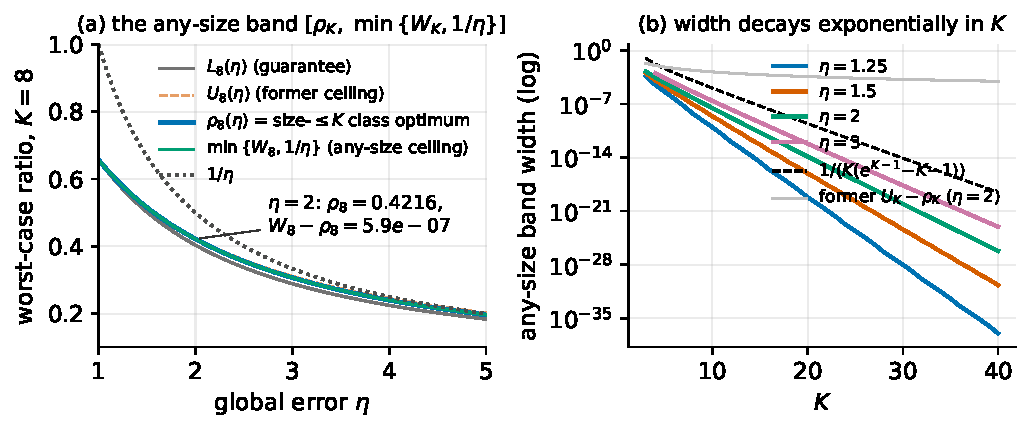
\includegraphics[width=\textwidth]{figures/sandwich_paper}
\caption{The two closures around predictive greedy at its own oracle
budget.
(a)~At $K=8$: the a priori guarantee $L_8$, the exact size-$\le K$ class
optimum $\rho_8$ (Theorem~\ref{thm:linear-exact}), the arbitrary-size
ceiling $\min\{W_8,1/\eta\}$ (Theorem~\ref{thm:linear-anysize}), the
former ceiling $U_8$ (thin dashed) and the unrestricted-query ceiling
$1/\eta$ (Theorem~\ref{thm:ceiling}).  The remaining band
$[\rho_8,\min\{W_8,1/\eta\}]$ (shaded) is narrower than the line width:
at $\eta=2$ its width is $5.9\cdot10^{-7}$.
(b)~Width of the arbitrary-size band against $K$ (log scale), computed
from the exact gap identity in rationals, with the theorem bound
$1/(K(e^{K-1}-K-1))$ dashed and the former $O(1/K^{2})$ width
$U_K-\rho_K$ in grey for comparison: the closure gained an exponential
factor.}
\label{fig:sandwich}
\end{figure}
|' \
%       main.tex > main_l3.tex
%   pdflatex -interaction=nonstopmode -jobname=main_l3 main_l3.tex  (x2)
%   rm main_l3.tex        # log kept as results/L3_compile.log
%
% Numbers note: as a results/ draft this file is outside the G3 audit scope;
% on wiring into main, the literals below (0.4216, 5.9e-7 at K=8/eta=2)
% must become numbers.tex macros per the CLAUDE.md rule.  Sources: rho_8(2)
% from results/L1_table.csv; W_8(2) - rho_8(2) printed by
% results/L3_sandwich_fig.py (exact-rational gap identity (17), ledger
% T10d).
%
% History: the previous version of this draft posed "settling the last
% O(1/K^2)" as the open problem.  That problem is now closed twice over:
% thm:linear-exact (ledger T10c) gives the exact value rho_K for the
% size-<=K class at every n >= 4K^5, and thm:linear-anysize (ledger T10d)
% caps the arbitrary-size linear class at rho_K plus an exponentially
% small term.  The successor open problem below is the one recorded on
% card T10d.

\paragraph{An open problem: the last exponentially small term.}
Within predictive greedy's own oracle budget the picture is now closed or
nearly closed on both readings of the query model.  If every query has
size at most $K$, Theorem~\ref{thm:linear-exact} gives the exact optimum:
no deterministic algorithm with at most $nK$ queries beats
$\rho_K(\eta)$ at any $n\ge4K^{5}$, and predictive greedy attains it.
If queries of arbitrary size are allowed, Theorem~\ref{thm:linear-anysize}
pins the $n\to\infty$ optimum $\alpha_{\mathrm{lin}}(K,\eta)$ into
\[
  \rho_K(\eta)\;\le\;\alpha_{\mathrm{lin}}(K,\eta)\;\le\;
  \rho_K(\eta)+\frac{1}{K\,(e^{K-1}-K-1)}
  \qquad(K\ge3),
\]
a band exponentially small in $K$ (Figure~\ref{fig:sandwich}); at $K=8$
and $\eta=2$ it has width $5.9\cdot10^{-7}$ above $\rho_8(2)=0.4216$.
What remains open is the last term: either remove it, proving
$\alpha_{\mathrm{lin}}(K,\eta)=\rho_K(\eta)$ outright, or exhibit a
linear-query algorithm whose worst-case ratio strictly exceeds
$\rho_K(\eta)$.  Two structural facts calibrate the difficulty.  The
upper-bound side cannot be settled by the present family shape: for
count-grid constructions whose predictor is a function of $|S|$ on all
sets with $|S\cap O|\le1$, of every size, the value
$W_K(\eta)>\rho_K(\eta)$ is optimal (the excess is forced, ledger T10d
and \texttt{results/Q3\_failure\_point.md}), so removing the term needs
either asymmetry or a different indistinguishability region.  The
algorithm side is constrained by finite evidence in the opposite
direction: every candidate examined so far, top-$(K{+}1)$ shortlists,
greedy-plus-swap, partial enumeration, and $\max$ of forward and reverse
greedy, falls back to $\rho_K$ or below once $n$ exceeds roughly $2K$
(ledger T11), and at small $n$ the comparison degenerates (exhaustive
search enters the budget; reverse greedy reads the hidden optimum off
the leaking large sets at $n<K+t^{\ast}$).  We do not presuppose which
way the term resolves.

% Draft caption for the paper-version sandwich figure
% (paper/figures/sandwich_paper.pdf, built by results/L3_sandwich_fig.py).
\begin{figure}[t]
\centering
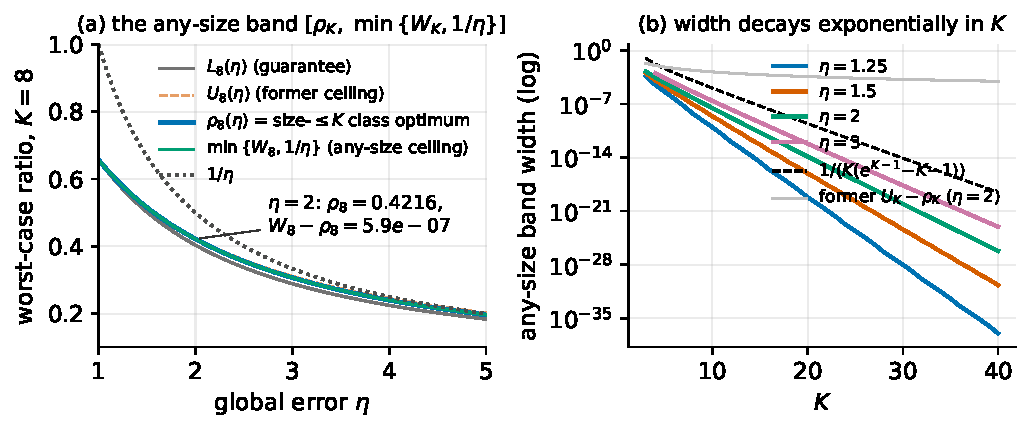
\includegraphics[width=\textwidth]{figures/sandwich_paper}
\caption{The two closures around predictive greedy at its own oracle
budget.
(a)~At $K=8$: the a priori guarantee $L_8$, the exact size-$\le K$ class
optimum $\rho_8$ (Theorem~\ref{thm:linear-exact}), the arbitrary-size
ceiling $\min\{W_8,1/\eta\}$ (Theorem~\ref{thm:linear-anysize}), the
former ceiling $U_8$ (thin dashed) and the unrestricted-query ceiling
$1/\eta$ (Theorem~\ref{thm:ceiling}).  The remaining band
$[\rho_8,\min\{W_8,1/\eta\}]$ (shaded) is narrower than the line width:
at $\eta=2$ its width is $5.9\cdot10^{-7}$.
(b)~Width of the arbitrary-size band against $K$ (log scale), computed
from the exact gap identity in rationals, with the theorem bound
$1/(K(e^{K-1}-K-1))$ dashed and the former $O(1/K^{2})$ width
$U_K-\rho_K$ in grey for comparison: the closure gained an exponential
factor.}
\label{fig:sandwich}
\end{figure}
|' \
%       main.tex > main_l3.tex
%   pdflatex -interaction=nonstopmode -jobname=main_l3 main_l3.tex  (x2)
%   rm main_l3.tex        # log kept as results/L3_compile.log
%
% Numbers note: as a results/ draft this file is outside the G3 audit scope;
% on wiring into main, the literals below (0.4216, 5.9e-7 at K=8/eta=2)
% must become numbers.tex macros per the CLAUDE.md rule.  Sources: rho_8(2)
% from results/L1_table.csv; W_8(2) - rho_8(2) printed by
% results/L3_sandwich_fig.py (exact-rational gap identity (17), ledger
% T10d).
%
% History: the previous version of this draft posed "settling the last
% O(1/K^2)" as the open problem.  That problem is now closed twice over:
% thm:linear-exact (ledger T10c) gives the exact value rho_K for the
% size-<=K class at every n >= 4K^5, and thm:linear-anysize (ledger T10d)
% caps the arbitrary-size linear class at rho_K plus an exponentially
% small term.  The successor open problem below is the one recorded on
% card T10d.

\paragraph{An open problem: the last exponentially small term.}
Within predictive greedy's own oracle budget the picture is now closed or
nearly closed on both readings of the query model.  If every query has
size at most $K$, Theorem~\ref{thm:linear-exact} gives the exact optimum:
no deterministic algorithm with at most $nK$ queries beats
$\rho_K(\eta)$ at any $n\ge4K^{5}$, and predictive greedy attains it.
If queries of arbitrary size are allowed, Theorem~\ref{thm:linear-anysize}
pins the $n\to\infty$ optimum $\alpha_{\mathrm{lin}}(K,\eta)$ into
\[
  \rho_K(\eta)\;\le\;\alpha_{\mathrm{lin}}(K,\eta)\;\le\;
  \rho_K(\eta)+\frac{1}{K\,(e^{K-1}-K-1)}
  \qquad(K\ge3),
\]
a band exponentially small in $K$ (Figure~\ref{fig:sandwich}); at $K=8$
and $\eta=2$ it has width $5.9\cdot10^{-7}$ above $\rho_8(2)=0.4216$.
What remains open is the last term: either remove it, proving
$\alpha_{\mathrm{lin}}(K,\eta)=\rho_K(\eta)$ outright, or exhibit a
linear-query algorithm whose worst-case ratio strictly exceeds
$\rho_K(\eta)$.  Two structural facts calibrate the difficulty.  The
upper-bound side cannot be settled by the present family shape: for
count-grid constructions whose predictor is a function of $|S|$ on all
sets with $|S\cap O|\le1$, of every size, the value
$W_K(\eta)>\rho_K(\eta)$ is optimal (the excess is forced, ledger T10d
and \texttt{results/Q3\_failure\_point.md}), so removing the term needs
either asymmetry or a different indistinguishability region.  The
algorithm side is constrained by finite evidence in the opposite
direction: every candidate examined so far, top-$(K{+}1)$ shortlists,
greedy-plus-swap, partial enumeration, and $\max$ of forward and reverse
greedy, falls back to $\rho_K$ or below once $n$ exceeds roughly $2K$
(ledger T11), and at small $n$ the comparison degenerates (exhaustive
search enters the budget; reverse greedy reads the hidden optimum off
the leaking large sets at $n<K+t^{\ast}$).  We do not presuppose which
way the term resolves.

% Draft caption for the paper-version sandwich figure
% (paper/figures/sandwich_paper.pdf, built by results/L3_sandwich_fig.py).
\begin{figure}[t]
\centering
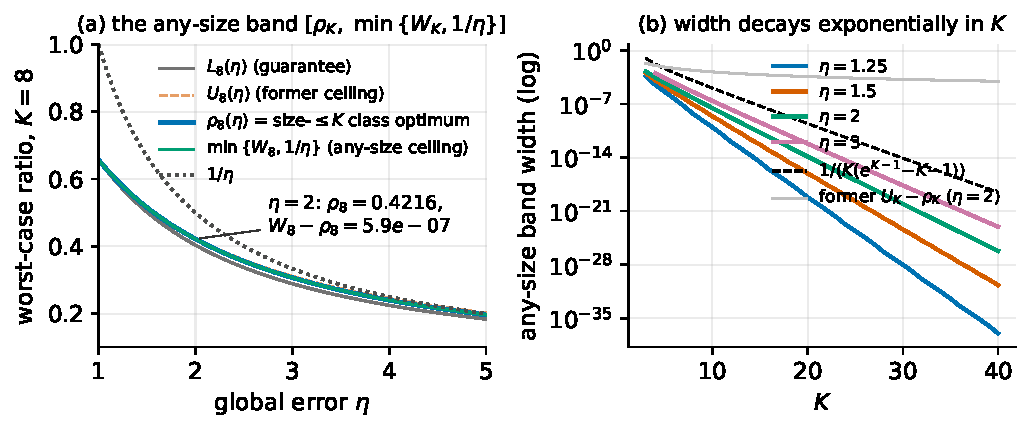
\includegraphics[width=\textwidth]{figures/sandwich_paper}
\caption{The two closures around predictive greedy at its own oracle
budget.
(a)~At $K=8$: the a priori guarantee $L_8$, the exact size-$\le K$ class
optimum $\rho_8$ (Theorem~\ref{thm:linear-exact}), the arbitrary-size
ceiling $\min\{W_8,1/\eta\}$ (Theorem~\ref{thm:linear-anysize}), the
former ceiling $U_8$ (thin dashed) and the unrestricted-query ceiling
$1/\eta$ (Theorem~\ref{thm:ceiling}).  The remaining band
$[\rho_8,\min\{W_8,1/\eta\}]$ (shaded) is narrower than the line width:
at $\eta=2$ its width is $5.9\cdot10^{-7}$.
(b)~Width of the arbitrary-size band against $K$ (log scale), computed
from the exact gap identity in rationals, with the theorem bound
$1/(K(e^{K-1}-K-1))$ dashed and the former $O(1/K^{2})$ width
$U_K-\rho_K$ in grey for comparison: the closure gained an exponential
factor.}
\label{fig:sandwich}
\end{figure}
|' \
%       main.tex > main_l3.tex
%   pdflatex -interaction=nonstopmode -jobname=main_l3 main_l3.tex  (x2)
%   rm main_l3.tex        # log kept as results/L3_compile.log
%
% Numbers note: as a results/ draft this file is outside the G3 audit scope;
% on wiring into main, the literals below (0.4216, 5.9e-7 at K=8/eta=2)
% must become numbers.tex macros per the CLAUDE.md rule.  Sources: rho_8(2)
% from results/L1_table.csv; W_8(2) - rho_8(2) printed by
% results/L3_sandwich_fig.py (exact-rational gap identity (17), ledger
% T10d).
%
% History: the previous version of this draft posed "settling the last
% O(1/K^2)" as the open problem.  That problem is now closed twice over:
% thm:linear-exact (ledger T10c) gives the exact value rho_K for the
% size-<=K class at every n >= 4K^5, and thm:linear-anysize (ledger T10d)
% caps the arbitrary-size linear class at rho_K plus an exponentially
% small term.  The successor open problem below is the one recorded on
% card T10d.

\paragraph{An open problem: the last exponentially small term.}
Within predictive greedy's own oracle budget the picture is now closed or
nearly closed on both readings of the query model.  If every query has
size at most $K$, Theorem~\ref{thm:linear-exact} gives the exact optimum:
no deterministic algorithm with at most $nK$ queries beats
$\rho_K(\eta)$ at any $n\ge4K^{5}$, and predictive greedy attains it.
If queries of arbitrary size are allowed, Theorem~\ref{thm:linear-anysize}
pins the $n\to\infty$ optimum $\alpha_{\mathrm{lin}}(K,\eta)$ into
\[
  \rho_K(\eta)\;\le\;\alpha_{\mathrm{lin}}(K,\eta)\;\le\;
  \rho_K(\eta)+\frac{1}{K\,(e^{K-1}-K-1)}
  \qquad(K\ge3),
\]
a band exponentially small in $K$ (Figure~\ref{fig:sandwich}); at $K=8$
and $\eta=2$ it has width $5.9\cdot10^{-7}$ above $\rho_8(2)=0.4216$.
What remains open is the last term: either remove it, proving
$\alpha_{\mathrm{lin}}(K,\eta)=\rho_K(\eta)$ outright, or exhibit a
linear-query algorithm whose worst-case ratio strictly exceeds
$\rho_K(\eta)$.  Two structural facts calibrate the difficulty.  The
upper-bound side cannot be settled by the present family shape: for
count-grid constructions whose predictor is a function of $|S|$ on all
sets with $|S\cap O|\le1$, of every size, the value
$W_K(\eta)>\rho_K(\eta)$ is optimal (the excess is forced, ledger T10d
and \texttt{results/Q3\_failure\_point.md}), so removing the term needs
either asymmetry or a different indistinguishability region.  The
algorithm side is constrained by finite evidence in the opposite
direction: every candidate examined so far, top-$(K{+}1)$ shortlists,
greedy-plus-swap, partial enumeration, and $\max$ of forward and reverse
greedy, falls back to $\rho_K$ or below once $n$ exceeds roughly $2K$
(ledger T11), and at small $n$ the comparison degenerates (exhaustive
search enters the budget; reverse greedy reads the hidden optimum off
the leaking large sets at $n<K+t^{\ast}$).  We do not presuppose which
way the term resolves.

% Draft caption for the paper-version sandwich figure
% (paper/figures/sandwich_paper.pdf, built by results/L3_sandwich_fig.py).
\begin{figure}[t]
\centering
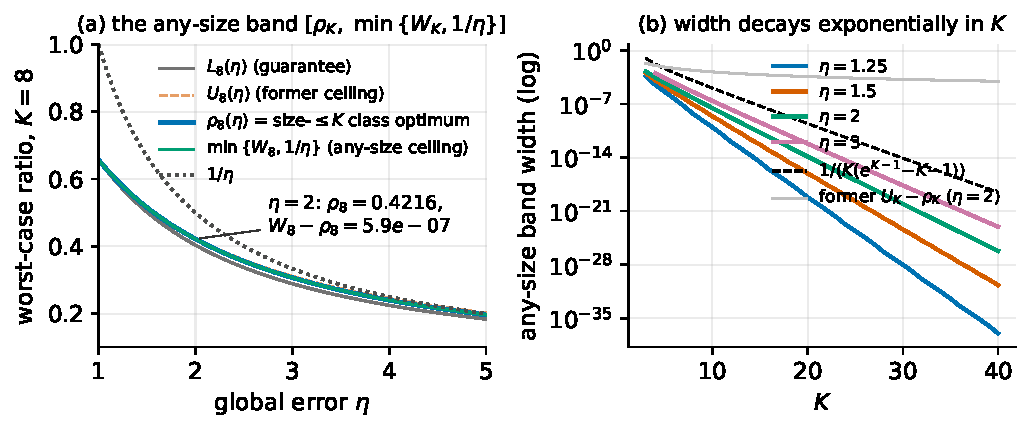
\includegraphics[width=\textwidth]{figures/sandwich_paper}
\caption{The two closures around predictive greedy at its own oracle
budget.
(a)~At $K=8$: the a priori guarantee $L_8$, the exact size-$\le K$ class
optimum $\rho_8$ (Theorem~\ref{thm:linear-exact}), the arbitrary-size
ceiling $\min\{W_8,1/\eta\}$ (Theorem~\ref{thm:linear-anysize}), the
former ceiling $U_8$ (thin dashed) and the unrestricted-query ceiling
$1/\eta$ (Theorem~\ref{thm:ceiling}).  The remaining band
$[\rho_8,\min\{W_8,1/\eta\}]$ (shaded) is narrower than the line width:
at $\eta=2$ its width is $5.9\cdot10^{-7}$.
(b)~Width of the arbitrary-size band against $K$ (log scale), computed
from the exact gap identity in rationals, with the theorem bound
$1/(K(e^{K-1}-K-1))$ dashed and the former $O(1/K^{2})$ width
$U_K-\rho_K$ in grey for comparison: the closure gained an exponential
factor.}
\label{fig:sandwich}
\end{figure}
